\documentclass[12pt, a4paper, twoside]{report} 
\usepackage{blindtext}
\usepackage{float}
\usepackage{setspace}
\linespread{1.5}
\usepackage{graphicx}
\usepackage[a4paper,top=3.5cm,bottom=3.5cm,left=2.5cm,right=2.5cm,marginparwidth=1.75cm]{geometry}
\setlength{\headheight}{14.5pt}
\usepackage[colorlinks=true, linkcolor=blue, citecolor=red]{hyperref}
\graphicspath{{./Chapter2/}}
\usepackage{acronym}
\usepackage{amsmath}
\usepackage{amssymb}
\usepackage{fancyhdr}
\usepackage{tikz}
\usepackage{colortbl} % Required for colored table rules
\usepackage{xcolor}    % Provides color definitions
\usepackage{mathtools}
\usepackage{subcaption}
\usepackage[compat=1.1.0]{tikz-feynman}
\definecolor{lightgray}{rgb}{0.8,0.8,0.8} 
\definecolor{verylightblue}{rgb}{0.90, 0.95, 1.0}
\usepackage{pifont}  % for \xmark
\newcommand{\cmark}{\checkmark}
\newcommand{\xmark}{\ding{55}}
\usepackage{adjustbox}
\usepackage[numbers,sort&compress]{natbib}
\usepackage{enumitem}
\setlist[itemize]{topsep=5pt, partopsep=0pt, parsep=0pt, itemsep=0.5\baselineskip}
\setlist[enumerate]{topsep=5pt, partopsep=0pt, parsep=0pt, itemsep=0.5\baselineskip}
\usepackage[perpage]{footmisc}
\usepackage{tablefootnote}
\usepackage{multirow}
\usepackage{longtable}
\usepackage{array}          % for better table formatting
\usepackage{booktabs}
\usepackage{makecell}

\setcounter{tocdepth}{4}     % Include subsubsections in TOC
\setcounter{secnumdepth}{4}  % Number subsubsections (optional)

\makeatletter
\g@addto@macro\normalsize{%
  \setlength{\abovedisplayskip}{1pt}%
  \setlength{\belowdisplayskip}{1pt}%
  \setlength{\abovedisplayshortskip}{1pt}%
  \setlength{\belowdisplayshortskip}{1pt}%
}
\makeatother

\usepackage{minitoc}

\usepackage{titlesec}
\titlespacing*{\subsection}{0pt}{1.5ex}{1ex}
\titlespacing*{\subsubsection}{0pt}{1.5ex}{1ex}

\usepackage{indentfirst}
\setlength{\parindent}{15pt}   % Indentation at beginning of paragraphs
\setlength{\parskip}{0.5em}    % Whitespace between paragraphs

\usepackage[Lenny]{fncychap}   % or whatever style you like

\newcommand{\circnum}[1]{%
  \tikz[baseline=(char.base)]{
    \node[shape=circle,draw,inner sep=1pt,minimum size=14pt] (char) {#1};}}

\makeatletter
\renewcommand{\DOCH}{%
    \@ifundefined{@chapapp}{\let\@chapapp\chaptername}{}%

    \settowidth{\px}{\CNV\FmN{\@chapapp}}%
    \addtolength{\px}{2pt}%
    \settoheight{\py}{\CNV\FmN{\@chapapp}}%
    \addtolength{\py}{1pt}%
    
    \settowidth{\mylen}{\CNV\FmN{\@chapapp}\space\CNoV\thechapter}%
    \addtolength{\mylen}{1pt}%
    \settowidth{\pxx}{\CNoV\thechapter}%
    \addtolength{\pxx}{-1pt}%
    
    \settoheight{\pyy}{\CNoV\thechapter}%
    \addtolength{\pyy}{-2pt}%
    \setlength{\myhi}{\pyy}%
    \addtolength{\myhi}{-1\py}%
    \par
    \parbox[b]{\textwidth}{%
        \rule[\py]{\RW}{\myhi}%
        \hskip -\RW%
        \rule[\pyy]{\px}{\RW}%
        \hskip -\px%
        \raggedright%
        \CNV\FmN{\@chapapp}\space\CNoV{\color{teal}\thechapter}%
        \hskip1pt%
        \mghrulefill{\RW}%
        \rule{\RW}{\pyy}\par\nobreak%
        \vskip -\baselineskip%
        \vskip -\pyy%
        \hskip \mylen%
        \mghrulefill{\RW}\par\nobreak%
        \vskip \pyy%
    }%
    \vskip 20\p@%
}
\makeatother

% thickness of the box‐rule (optional; adjust to your taste)
\ChNameUpperCase

\ChNameVar{\fontsize{14}{16}\selectfont}
\ChNumVar{\fontsize{60}{62}\selectfont}
\ChTitleVar{\Huge\bfseries}
\ChRuleWidth{1.15pt}

%-------------
% CMS Packages
\usepackage{style/ptdr-definitions}
\usepackage{style/hepparticles}
\usepackage{style/heppennames2}
\usepackage{mathrsfs}
%-------------

\pagestyle{plain}  % Default plain page style
\fancypagestyle{chapterpages}{
    \fancyhf{} % Clear existing header/footer
    \fancyhead[L]{\thepage}  % Left header: Page number
    \fancyhead[R]{\nouppercase{Chapter \thechapter: \leftmark}}
    \renewcommand{\headrulewidth}{0.4pt} % Header rule
}
\renewcommand{\chaptermark}[1]{\markboth{#1}{}}

\newcommand{\hardmaths} {\frac{\sin{(x\pi)}} {2\alpha}}

\newcommand{\diff}[2]  {\frac{\textrm{d}{#1}} {\textrm{d}{#2}}}

% ===== Consistent spacing around math environments =====
\newenvironment{equation_pad}
  {\vspace{-0.5pt}\begin{equation}}
  {\end{equation}\vspace{-0.5pt}}

\newenvironment{align_pad}
  {\vspace{-0.5pt}\begin{align}}
  {\end{align}\vspace{-0.5pt}}

\newenvironment{gather_pad}
  {\vspace{-0.5pt}\begin{gather}}
  {\end{gather}\vspace{-0.5pt}}

\newenvironment{multline_pad}
  {\vspace{-0.5pt}\begin{multline}}
  {\end{multline}\vspace{-0.5pt}}


\begin{document}
\pagenumbering{roman} 
\dominitoc


\includegraphics[width=7cm]{IMPERIAL_Wordmark_CMYK_Blue_safe_area_2024.jpg}
\vspace{5cm}
\begin{center}


{\huge Exploring extended Higgs sectors and the CP Nature of the Higgs Yukawa coupling using tau leptons at the CMS Experiment}
\rule{15cm}{1pt}
\vspace{2cm}

Klitos Savva\\
2025
\vspace{2cm}

Department of Physics

Imperial College London
\vspace{2cm}

A thesis submitted in fulfilment of the requirements \\ for the degree of
Doctor of Philosophy at Imperial College London\\
\vfill
\clearpage
\end{center}

\chapter*{Abstract}
Since the discovery of the Higgs boson at the LHC, attention has turned to testing its properties and searching for extended Higgs sectors that could reveal new physics. This thesis addresses three complementary topics within the CMS experiment: the study of a compact data format to meet the ever-growing computing needs, a direct search for additional Higgs bosons in the four-tau final state, and a precision measurement of the CP structure of the Higgs–tau Yukawa coupling. First, the development of the compact RAW' data format is described, demonstrating recovered performance in displaced track reconstruction and positioning RAW' as a promising option. Second, a search for additional Higgs bosons in the four-tau final state is performed using the full Run 2 dataset of $137\unit{fb}^{-1}$ at $\sqrt{s}=13\TeV$. No excess is observed, and exclusion limits on $Z^* \to \phi A \to 4\tau$ production reach from $\mathcal{O}(190\unit{fb})$ at low masses to $\mathcal{O}(0.4\unit{fb})$ at high masses. Regions of the Type-X 2HDM relevant to the muon anomalous magnetic moment are also excluded. Finally, a measurement of the CP structure of the Higgs–tau Yukawa coupling is performed in the $\tauh\tauh$ channel with Run 3 data, excluding the pure CP-odd hypothesis at $1.74\sigma$. When combined with the Run 2 result, the exclusion improves to $3.55\sigma$ with $\alpha^{\PH\tau\tau}$ constrained to $\pm 15^\circ$, representing the most precise determination to date. This result remains compatible with the SM prediction of a CP-even coupling.

\chapter*{Statement of Originality}

I declare that the work presented in this thesis is my own. Wherever figures, tables, or results have been taken from other sources, this is clearly indicated by a reference in the text or figure caption. Figures labelled ``CMS'' are sourced from CMS publications. The ``CMS preliminary'' label is attached to CMS public results that are not yet finalised by the Collaboration or the journal. The ``Simulation'' tag is used when only simulated data is shown in a CMS public plot. Figures labelled as ``Private work (CMS data/simulation)'' or ``Private work (CMS simulation)'' indicate non-public material; in the context of this thesis, these correspond to results currently under review by the CMS Collaboration. 

Chapters~1-4 do not contain original research by myself; rather, they provide essential background, covering the theoretical motivations, experimental apparatus, and methods used to produce and collect the data analysed in this thesis.  

The work in Chapter~5 forms part of my CMS ``service work'' and was carried out with the guidance of Dr.~Marco Musich. While the initial development was collaborative, the second iteration of the redefined data format presented in this chapter was conducted by myself.  

Chapter~6 describes a search for extended Higgs sector signatures, conducted in collaboration with members of the Imperial College London $H\to\tau\tau$ group, namely Dr.~George Uttley and Dr.~Daniel Winterbottom. I contributed across the full analysis workflow, from the implementation of the framework to the interpretation of the final results. My specific focus was on background modelling, optimisation strategies, uncertainty estimation, and the statistical interpretation of the results.  

The final analysis chapter presents a measurement of the CP structure of the Higgs-tau Yukawa coupling in $H\to\tau_h\tau_h$ decays, carried out in collaboration with other members of the CMS $H\to\tau\tau$ group. This particular channel was primarily developed by the Imperial College team consisting of Lucas Russell, Dr.~Daniel Winterbottom, and myself. I contributed to all stages of the analysis workflow, with particular responsibility for setting up the framework, generating signal simulations, and optimising analysis cuts and techniques (including the development of the improved $X$-$a_1$ method, which was my own work). In addition, I contributed to the background modelling and the statistical interpretation of the results.  


\tableofcontents
\listoffigures
\listoftables

\clearpage
\section*{List of Acronyms}
\begin{acronym}
\acro{SM}{Standard Model}
\acro{BSM}{Beyond-the-Standard Model}
\acro{QFT}{Quantum Field Theory}
\acro{QED}{Quantum Electrodynamics}
\acro{QCD}{Quantum Chromodynamics}
\acro{BEH}{Brout-Englert-Higgs}
\acro{SSB}{Spontaneous Symmetry Breaking}
\acro{VEV}{Vacuum Expectation Value}
\acro{dof}{Degrees of Freedom}
\acro{LHC}{Large Hadron Collider}
\acro{ggH}{Gluon-gluon fusion}
\acro{VBF}{Vector boson fusion}
\acro{VH}{Vector boson associated production}
\acro{EFT}{Effective Field Theory}
\acro{SUSY}{Supersymmetry}
\acro{MSSM}{Minimal Supersymmetric Standard Model}
\acro{2HDM}{Two-Higgs Doublet Model}
\acro{FCNC}{Flavour-Changing-Neutral-Currents}
\acro{CMS}{Compact Muon Solenoid}
\acro{MET}{Missing Transverse Energy}
\acro{CERN}{European Organization for Nuclear Research}
\acro{LEP}{Large Electron Positron}
\acro{LINAC4}{Linear Accelerator 4}
\acro{PSB}{Proton Synchrotron Booster}
\acro{PS}{Proton Synchrotron}
\acro{SPS}{Super Proton Synchrotron}
\acro{PU}{Pileup}
\acro{ECAL}{Electromagnetic Calorimeter}
\acro{HCAL}{Hadronic Calorimeter}
\acro{BPIX}{Barrel Pixel}
\acro{FPIX}{Forward Pixel}
\acro{SST}{Silicon Strip Tracker}
\acro{TIB}{Tracker Inner Barrel}
\acro{TID}{Tracker Inner Disks}
\acro{TOB}{Tracker Outer Barrel}
\acro{TEC}{Tracker EndCaps}
\acro{APD}{Avalanche Photodiode}
\acro{VPT}{Vacuum Phototriode}
\acro{HB}{Hadron Barrel}
\acro{HE}{Hadron Endcap}
\acro{HO}{Hadron Outer}
\acro{HF}{Hadron Forward}
\acro{DT}{Drift Tube}
\acro{CSC}{Cathode Strip Chamber}
\acro{RPC}{Resistive Plate Chamber}
\acro{L1}{Level-1}
\acro{HLT}{High Level Trigger}
\acro{WP}{Working Point}
\acro{CTF}{Combinatorial Track Finder}
\acro{KF}{Kalman Filter}
\acro{PV}{Primary Vertex}
\acro{GSF}{Gaussian-sum Filter}
\acro{PF}{Particle Flow}
\acro{MVA}{Multivariate Analysis}
\acro{BDT}{Boosted Decision Tree}
\acro{CHS}{Charged Hadron Subtraction}
\acro{PUPPI}{Pileup Per Particle Identification}
\acro{SV}{Secondary Vertex}
\acro{IP}{Impact Parameter}
\acro{HPS}{Hadron-Plus Strips}
\acro{DM}{Decay Mode}
\acro{FED}{Front End Driver}
\acro{PDF}{Parton Distribution Function}
\acro{MC}{Monte Carlo}
\acro{ISR}{Initial-State Radiation}
\acro{FSR}{Final-State Radiation}
\acro{LO}{Leading Order}
\acro{NLO}{Next-to-Leading Order}
\acro{NNLO}{Next-to-Next-to-Leading Order}
\acro{DY}{Drell-Yan}
\acro{SF}{Scale-Factor}
\acro{TES}{Tau Energy Scale}
\acro{DR}{Determination Region}
\acro{AR}{Application Region}
\acro{SR}{Signal Region}
\acro{ML}{Machine Learning}
\acro{P.D.F}{Probability Distribution Function}
\acro{AMS}{Approximate Median Significance}
\acro{HL}{High Luminosity}
\acro{ZMF}{Zero-Momentum Frame}
\acro{P.V.}{Polarimetric Vector}
\acro{NP}{Neutral-Pion}
\acro{CDF}{Cumulative Distribution Function}
\end{acronym}

\clearpage
\pagenumbering{arabic}
\setcounter{page}{1}

\setcounter{mtc}{1}
\chapter{The Standard Model of particle physics}

The \ac{SM} of particle physics is our current best theoretical framework underpinning our understanding of the subatomic world, providing a description of fundamental elementary particles and their interactions via the electromagnetic force, weak nuclear force and the strong nuclear force. The fourth fundamental force of nature, Gravity, is absent from the SM, highlighting one of its key limitations. However, in high-energy physics experiments, where the interactions of subatomic particles are being studied, the omission of gravity is considered a safe simplification. Extremely powerful predictions have emerged from this theoretical framework, with its greatest success being the discovery of the Higgs boson by the ATLAS and CMS Collaborations in 2012, completing the observational confirmation of all hypothesized SM particles. Despite its success, the Standard Model has its limitations. Along with the absence of gravity, it leaves several fundamental questions unanswered, such as the nature of neutrino oscillations, the existence of dark matter, the hierarchy problem, and the matter-antimatter asymmetry in the universe, which cannot be fully explained by the predicted amount of CP violation, driving the field to look for explanations beyond the SM. In the pursue of \ac{BSM} physics, a deep understanding of the SM theory is crucial. This is the goal of this chapter aiming to establish the base foundation for this work, the SM, taking a trip down the fundamental blocks of the theory, including its particle content, interactions, and the Higgs mechanism.

\section{Particle content}

\begin{figure}
\centering
\includegraphics[width= 1\textwidth]{Figures/Introduction/Particles.pdf}
\end{figure}

\section{Fundamental forces}
\section{Higgs mechanism}
\section{The Higgs boson}

\cite{Rowling_1997}
\cite{Thor_2011}
\setcounter{mtc}{2}
\chapter{Motivation for Higgs Sector Extensions and Higgs CP Studies}
\chaptermark{Motivation for Higgs Sector Extensions and Higgs CP Studies}  
\thispagestyle{plain}  % First page has default style
\pagestyle{chapterpages}
\label{Section:Chapter2}

In Chapter~\ref{Section:Chapter1}, the SM of particle physics was explored to establish the theoretical foundation of this work. While the SM has been immensely successful, with its predictions verified experimentally to a high degree of precision, it remains an incomplete theory of nature due to several fundamental theoretical problems. Beyond these theoretical issues, the emergence of experimental results in tension with SM predictions has sparked significant interest. Although the statistical significance of these tensions is not yet sufficient to claim new discoveries, the search for BSM physics to explain them remains an intriguing and active area of research. This chapter will focus on two major theoretical challenges; the hierarchy problem and the observed matter-antimatter asymmetry of the universe, while also discussing key experimental tensions. Possible solutions within the context of BSM physics will then be explored, with the observed Higgs boson playing an integral role in the matter-antimatter asymmetry discussion.

\section{Hierarchy problem}

A fundamental principle in theoretical physics is naturalness, which suggests that parameters in a theory should not take values that are unnaturally small or large without an underlying reason. In the case of the Standard Model (SM), this concept is particularly relevant to the Higgs boson mass, which is significantly smaller than the Planck scale ($m_P \approx 10^{19} \GeV$), where gravitational interactions become as strong as other fundamental forces.

Since the SM is widely regarded as an effective field theory (EFT), valid up to a certain energy scale, it is expected to require an extension at higher energies. The hierarchy problem arises from the absence of a natural mechanism to prevent large quantum corrections from driving the Higgs boson mass to much higher scales, typically near the Planck mass. This extreme disparity between the electroweak scale ($10^2 \GeV$) and the Planck scale remains one of the most significant unresolved questions in high-energy physics.

In QFT, the Higgs boson mass in not simply a fixed parameter. It receives corrections to its physical mass from virtual processes involving particles that couple directly or indirectly to the Higgs field. Mathematically the physical mass of the Higgs boson can be expressed as

\begin{equation}
    m_H^2 = (m_H^0)^2 + \Delta m_H^2
\label{Equation:Chapter2_HiggsBosonMass}
\end{equation}

where $m_H^0$ represents the bare mass of the Higgs boson, and $\Delta m_H$ term encapsulates the quantum loop corrections. In the EFT framework, the loop-induced correction term takes the form,

\begin{equation}
    \Delta m_H^2 = -\frac{g_f^2}{8\pi^2}\Lambda^2 + \space \text{...}
\end{equation}

where $\Lambda$ should be interpreted as the least energy scale at which new physics is expected to modify the high-energy behaviour of the theory~\cite{SUSY}. The Feynman diagram for the mass correction due to a fermion coupling to the Higgs field is shown in Fig.~\ref{Figure:Chapter2_Hierarchy_Feynman1}.

\begin{figure}[h]
\centering
\begin{tikzpicture}
    \begin{feynman}
      \vertex[blob, minimum size=2.5cm] (m) at ( 0, 0) {};
      \vertex[blue] (a) at (-3,0){\(H\)};
      \vertex[blue] (b) at ( 3,0){\(H\)};
      \node[black] at (0,1.5) {f}; 


      \diagram* {
        (a) -- [scalar] (m) -- [scalar] (b),
      };
    \end{feynman}
\end{tikzpicture}

\caption{One-loop Feynman diagram illustrating the correction to the Higgs boson mass due to its coupling to a fermion.}
\label{Figure:Chapter2_Hierarchy_Feynman1}
\end{figure}

At the core of the hierarchy problem lies this $\Lambda$ term. If $\Lambda$ is taken to be close to the Plank scale, these quantum loop correction become many orders of magnitude larger than the observed mass of the Higgs boson, $125.04 \pm 0.12~\GeV$ (in natural units)~\cite{Higgs_Mass_Z4L}. To reconcile this, an extreme degree of fine-tuning in Eq.~\ref{Equation:Chapter2_HiggsBosonMass} is required. Specifically, the bare mass term has to be sufficiently large ($\mathcal{O}(10^{38})$) to cancel out the quantum loop correction term. This degree of unnatural finetuning remains an open question in the field, as the Higgs mass would otherwise be expected close to the scale of new physics. This could suggest that new physics may exist near $\Lambda$, that can stabilise the Higgs mass and resolve the hierarchy problem. 

Perhaps, the most studied and appealing solution to the hierarchy problem is \ac{SUSY}~\cite{SUSY}, which introduces a symmetry relating fermions and bosons. In SUSY, every known SM particle has at least one supersymmetric partner. Bosons have fermionic superpartners while, fermions have scalar boson superpartners. This symmetry provides a natural way of addressing this extreme fine-tuning, as superpartners also contribute to $\Delta m_H^2$ but, with opposite signs relative to their SM counterparts. This allows the Higgs mass to stabilise naturally through the cancellation of the quantum loop corrections. The Feynman diagram for the mass correction due to a fermionic superpartner (scalar boson) is shown in Fig.~\ref{Figure:Chapter2_Hierarchy_Feynman2}.

\begin{figure}[h]
\centering
\begin{tikzpicture}
    \begin{feynman}
      \vertex[blob, minimum size=2.5cm] (m) at ( 0, 0) {};
      \vertex[blue] (a) at (-3,-1.29){\(H\)};
      \vertex[blue] (b) at ( 3,-1.29){\(H\)};

      \diagram* {
        (m),
        (a) -- [scalar] (b),
      };
    \end{feynman}
\end{tikzpicture}

\caption{One-loop correction to the Higgs mass due to a scalar S}
\label{Figure:Chapter2_Hierarchy_Feynman2}
\end{figure}

While SUSY provides a natural solution to the hierarchy problem, the lack of any experimental evidence for supersymmetric partners, along with strong experimental constraints on the simplest SUSY extension of the SM (MSSM), has lead to alternative extensions to the SM Higgs sector gaining traction. One such extension is the \ac{2HDM}, where the introduction of additional Higgs bosons that could alter the running of coupling constants and loop corrections. Moreover, 2HDMs are particularly interesting in light of the muon $g-2$ anomaly, which will be discussed in this chapter.

\section{Extended Higgs sector - 2HDM}
\label{Section:Chapter2_2HDM}
The simplest extension to the SM Higgs sector is the 2HDM~\cite{2HDM_1}. In contrast to the SM, the 2HDM introduces two complex scalar $\mathcal{SU(2)}_L$ doublets, $\Phi_1$ and $\Phi_2$.

\begin{equation}
\Phi_i =
\begin{pmatrix}
\phi_i^{+} \\
\phi_i^{0} 
\end{pmatrix}
\quad ,\quad i = 1,2
\end{equation}

The presence of the additional doublet in 2HDM leads to a richer potential structure. The general 2HDM Higgs potential, written in terms of the doublets $\Phi_1$ and $\Phi_2$, takes the form,

\begin{equation}
\begin{array}{c}
    V(\Phi_1,\Phi_2) = m_{11}^2 \Phi_1^{\dagger}\Phi_1 + m_{22}^2 \Phi_2^{\dagger}\Phi_2 - m_{12}^2(\Phi_1^\dagger\Phi_2 + \text{H.c.}) \\
    + \frac{1}{2} \lambda_1(\Phi_1^\dagger\Phi_1)^2 + \frac{1}{2}\lambda_2(\Phi_2^\dagger\Phi_2)^2 + \lambda_3(\Phi_1^\dagger\Phi_1)(\Phi_2^\dagger\Phi_2) \\
    + \lambda_4(\Phi_1^\dagger\Phi_2)(\Phi_2^\dagger\Phi_1) + \frac{1}{2}\lambda_5[(\Phi_1^\dagger\Phi_2)^2 + (\Phi_2^\dagger\Phi_1)^2] \\
    + \lambda_6(\Phi_1^\dagger\Phi_1)(\Phi_1^\dagger\Phi_2) + \lambda_7(\Phi_2^\dagger\Phi_2)(\Phi_1^\dagger\Phi_2)
\end{array}
\end{equation}

where the scalar potential is expressed in terms of the mass parameters ($m_{ij}$) and the quartic couplings ($\lambda_i$)~\cite{2HDM_1}. 

A major constraint imposed in 2HDMs is the suppression of tree-level \ac{FCNC}~\cite{FCNC_1,2HDM_2}. In a generic 2HDM, both Higgs doublets can couple to the same fermion flavour, which leads to non-diagonal Yukawa couplings after SSB. These couplings are strongly constrained by experimental data~\cite{FCNC_Constraints}. To forbid these tree-level interactions, a discrete $\mathbb{Z}_2$ symmetry \cite{2HDM_2} is introduced, 

\begin{equation}
    \Phi_1 \to \Phi_1, \Phi_2 \to - \Phi_2, \Phi_1 \not\to \Phi_2 
\end{equation}

This ensures that each fermion type couples to only one of the Higgs doublets. Following the introduction of the discrete symmetry, the quartic interaction terms $\lambda_6$ and $\lambda_7$ are eliminated from the potential. In addition to suppressing flavor-changing neutral currents (FCNCs), charge-parity (CP) symmetry plays a crucial role in ensuring the theoretical consistency of 2HDMs. CP symmetry is a fundamental symmetry in quantum field theory (QFT) that combines charge conjugation (C) and parity (P). Under a charge conjugation transformation, particles are transformed into their corresponding antiparticles whilst, parity transformations invert the spatial coordinates. In the 2HDM, CP conservation is often imposed to prevent spontaneous CP violation by requiring all free parameters in the Higgs potential to be real.

In the 2HDM, electroweak symmetry breaking occurs similarly to the SM. To preserve the $\mathcal{U}(1)_{\text{EM}}$ gauge symmetry, only the neutral components of the Higgs doublets acquire non-zero VEVs, ensuring that the photon remains massless. The vacuum structure is given by,

\begin{equation}
    <0|\Phi_i|0> = \frac{1}{\sqrt{2}} \begin{pmatrix}
        0 \\
        \nu_i
    \end{pmatrix} \quad,\quad i=1,2
\end{equation}

where $\nu_1$ and $\nu_2$ are the VEVs associated with each Higgs doublet.

After SSB, the Higgs doublets can be expanded around the minima

\begin{equation}
    \text{SSB} \rightarrow\Phi_i = \begin{pmatrix}
        \phi_i^+ \\
        \frac{1}{\sqrt{2}}(\nu_i + h_i + iz_i)
    \end{pmatrix} \quad,\quad i=1,2
\end{equation}

where the doublets have been expressed in terms of CP-even ($h_i$), CP-odd ($z_i$) and charged Higgs fields ($\phi_i^+$).

Analogous to the SM Higgs sector, the introduction of a second Higgs doublet introduces an additional four dof. Upon SSB, three out of the eight dof are absorbed as Goldstone bosons providing the $\PW^{\pm}$ and $\PZ$ bosons with longitudinal dof while the remaining five dof correspond to five physical Higgs bosons; two CP-even ($\Ph$ and $\PH$), one CP-odd (A) and two charged Higgs bosons ($\PH^{\pm}$). The mass eigenstates corresponding to these physical Higgs bosons are admixtures of the components of the two Higgs doublets,

\begin{equation}
\begin{array}{c}
     h = h_1 \sin{\alpha} - h_2 \cos{\alpha} \\
     H = - h_1 \cos{\alpha} - h_2 \sin{\alpha} \\
     H^\pm = \phi_1^+ \sin{\beta} + \phi_2^+ \cos{\beta} \\
     A = z_1 \sin{\beta} - z_2 \cos{\beta}
\end{array}
\label{Equation:Chapter2_2HDM-MassEigenstates}
\end{equation}

where the parameter $\alpha$ governs the mixing between the CP-even scalars and $\beta$ is a rotational angle that diagonalises the mass-squared matrices of the pseudoscalar and the charged Higgs. The latter is defined as,

\begin{equation}
    \tan{\beta} = \nu_2/\nu_1
\end{equation}

To ensure the theoretical consistency and predictability within the 2HDM, the degree of mixing needs to be carefully controlled. This is achieved once again through a discrete $\mathbb{Z}_2$ symmetry. However, rather being strictly imposed, the symmetry is softly broken by the $m_{12}^2$ term in the scalar potential. This soft-breaking of the symmetry allows the Yukawa couplings to remain flavour diagonal while, simultaneously allowing for mass mixing between the Higgs doublets ($\Phi_i$). CP-conserving 2HDMs are split in different types, which are defined based on which Higgs doublet couples to each fermion flavour. The four types of CP-conserving 2HDMs are shown in Table~\ref{Table:Chapter2_2HDM-Types}.

\begin{table}[h]
\centering
\renewcommand{\arraystretch}{1.5} % Increase row height
\setlength{\tabcolsep}{12pt} % Increase column width
\arrayrulecolor{black} % Ensure outer borders are black
\begin{tabular}{|c|c|c|c|c|}
\hline
    & Type I   & Type II  & Type X   & Type Y   \\ \hline \hline
$u$ & $\Phi_2$ & $\Phi_2$ & $\Phi_2$ & $\Phi_2$ \\ 
\arrayrulecolor{lightgray} \hline
$d$ & $\Phi_2$ & $\Phi_1$ & $\Phi_2$ & $\Phi_1$ \\ 
\arrayrulecolor{lightgray} \hline
$l$ & $\Phi_2$ & $\Phi_2$ & $\Phi_1$ & $\Phi_2$ \\ 
\arrayrulecolor{black} \hline
\end{tabular}
\caption{Table showing how each Higgs doublet couples to each fermion flavour in different 2HDM types.}
\label{Table:Chapter2_2HDM-Types}
\end{table}

In each 2HDM type, the structure of the Yukawa interactions depends on the specific assignment of the fermion couplings to the Higgs doublets. After SSB, the Yukawa part of the 2HDM Lagrangian can be expressed in terms of the physical Higgs mass eigenstates, up-like ($u$) and down-like($d$) quark, charged lepton ($l$) and neutrino ($\upsilon$) fields as

\begin{equation}
\begin{aligned}
    \text{SSB} \rightarrow \mathcal{L}_{Yukawa}^{2HDM} &= - \sum\limits_{f=u,d,l} \frac{m_f}{\nu} 
    \left(g_f^h \overline{f}f h + g_f^H\overline{f}f H - i g_f^A\overline{f} \gamma_5 f A \right) \\
    &\quad - \left\{ \frac{\sqrt{2}V_{ud}}{\nu} \overline{u} 
    \left(m_u g_u^A P_L + m_d g_d^A P_R \right) d H^+ \right. \\
    &\quad \left. + \frac{\sqrt{2}m_l g_{l}^A}{\nu} \overline{\upsilon
_L} l_R H^+ + H.c. \right\}
\end{aligned}
\label{Equation:Chapter2_2HDM-YukawaLagrangian}
\end{equation}

where $g_f^H,g_f^A,g_f^h$ are the normalised Yukawa couplings of the fermions to the Higgs mass eigenstates, expressed relative to the SM Higgs boson's couplings. These couplings are summarised in Table~\ref{Table:Chapter2_2HDM-Couplings} for each of the four types of 2HDMs.


\begin{table}[h]
\centering
\renewcommand{\arraystretch}{1.5} % Increase row height
\setlength{\tabcolsep}{12pt} % Increase column width
\arrayrulecolor{black} % Ensure outer borders are black
\begin{tabular}{|c|c|c|c|c|}
\hline
        & Type I                     & Type II                     & Type X                                        & Type Y                      \\ \hline \hline
$g_l^A$ & $1/\tan{\beta}$            & $\tan{\beta}$               & $\tan{\beta}$    & $-1/\tan{\beta}$            \\ \arrayrulecolor{lightgray} \hline
$g_u^A$ & $1/\tan{\beta}$            & $1/\tan{\beta}$             & $1/\tan{\beta}$                               & $1/\tan{\beta}$             \\ \arrayrulecolor{lightgray} \hline
$g_d^A$ & $1/\tan{\beta}$            & $\tan{\beta}$               & $-1/\tan{\beta}$                              & $\tan{\beta}$               \\ \arrayrulecolor{lightgray} \hline
$g_l^H$ & $\sin{\alpha}/\sin{\beta}$ & $\cos{\alpha}/\cos{\beta}$  & $\cos{\alpha}/\cos{\beta}$                    & $\sin{\alpha}/\sin{\beta}$  \\ \arrayrulecolor{lightgray} \hline
$g_u^H$ & $\sin{\alpha}/\sin{\beta}$ & $\sin{\alpha}/\sin{\beta}$  & $\sin{\alpha}/\sin{\beta}$                    & $\sin{\alpha}/\sin{\beta}$  \\ \arrayrulecolor{lightgray} \hline
$g_d^H$ & $\sin{\alpha}/\sin{\beta}$ & $\cos{\alpha}/\cos{\beta}$  & $\sin{\alpha}/\sin{\beta}$                    & $\cos{\alpha}/\cos{\beta}$  \\ \arrayrulecolor{lightgray} \hline
$g_l^h$ & $\cos{\alpha}/\sin{\beta}$ & $-\sin{\alpha}/\cos{\beta}$ & $-\sin{\alpha}/\cos{\beta}$                   & $\cos{\alpha}/\sin{\beta}$  \\ \arrayrulecolor{lightgray} \hline
$g_u^h$ & $\cos{\alpha}/\sin{\beta}$ & $\cos{\alpha}/\sin{\beta}$  & $\cos{\alpha}/\sin{\beta}$                    & $\cos{\alpha}/\sin{\beta}$  \\ \arrayrulecolor{lightgray} \hline
$g_d^h$ & $\cos{\alpha}/\sin{\beta}$ & $-\sin{\alpha}/\cos{\beta}$ & $\cos{\alpha}/\sin{\beta}$                    & $-\sin{\alpha}/\cos{\beta}$ \\ \arrayrulecolor{black} \hline
\end{tabular}
\caption{Table summarising the couplings of the different fermion groups to the neutral Higgs bosons for different 2HDM types.}
\label{Table:Chapter2_2HDM-Couplings}
\end{table}

In 2HDMs, the observed Higgs boson can be matched to the predicted CP-even bosons by a linear combination of the two mass eigenstates 

\begin{equation}
    h_{\text{obs}} = \sin{(\beta - \alpha)} h + \cos{(\beta - \alpha)} H 
\end{equation}

In the Higgs alignment limit, one of these CP-even neutral Higgs boson is the observed Higgs, which enables two possible alignment scenarios, the normal and inverted scenarios. In the normal scenario, the observed Higgs is identified as the lighter h, in contrast to H being identified as the observed Higgs in the inverted scenario. The couplings of the unmatched CP-even boson are summarised in Table~\ref{Table:Chapter2_2HDM-CouplingsAlignmentLimit} for each of the four different types of 2HDMs.

\begin{equation}
\begin{rcases}
  h_{\text{obs}} = h \\
  \cos(\beta-\alpha) = 0 
\quad \end{rcases}
\quad \text{Normal}
\label{Equation:Chapter2-NormalScenario}
\end{equation}

\begin{equation}
\begin{rcases}
  h_{\text{obs}} = H \\
  \sin(\beta-\alpha) = 0
\quad \end{rcases}
\quad \text{Inverted}
\label{Equation:Chapter2-InvertedScenario}
\end{equation}


\begin{table}[h]
\centering
\renewcommand{\arraystretch}{1.5} % Increase row height
\setlength{\tabcolsep}{12pt} % Increase column width
\arrayrulecolor{black} % Ensure outer borders are black
\begin{tabular}{|c|c|c|c|c|}
\hline
Normal (Inverted)     & Type I                     & Type II                     & Type X                                        & Type Y                      \\ \hline \hline
(-)$g_l^{H(h)}$ & $-1/\tan{\beta}$  & $\tan{\beta}$  & $\tan{\beta}$                    & $-1/\tan{\beta}$  \\ \arrayrulecolor{lightgray} \hline
(-)$g_u^{H(h)}$ & $-1/\tan{\beta}$  & $-1/\tan{\beta}$  & $-1/\tan{\beta}$                    & $-1/\tan{\beta}$  \\ \arrayrulecolor{lightgray} \hline
(-)$g_d^{H(h)}$ & $-1/\tan{\beta}$  & $\tan{\beta}$  & $-1/\tan{\beta}$                    & $\tan{\beta}$  \\ \arrayrulecolor{black} \hline
\end{tabular}
\caption{Table showing the couplings of different fermion groups to the neutral Higgs boson (not matched to the observed Higgs) for different 2HDM types. Couplings for both normal and inverted scenarios are shown in a simplified format using Eqs.~\ref{Equation:Chapter2-NormalScenario}-\ref{Equation:Chapter2-InvertedScenario}.}
\label{Table:Chapter2_2HDM-CouplingsAlignmentLimit}
\end{table}

\section{\texorpdfstring{Muon $g$-2 anomaly}{Muon g-2 anomaly}}

In 2023, Fermilab announced the most precise measurement of the anomalous magnetic moment of the muon, $\alpha_\mu$~\cite{Fermilab_g-2}. Combined with the earlier result from the Brookhaven National Laboratory, the experimental average of the muon anomaly exhibits a 5.0 standard deviations from SM prediction compiled by the Muon $g-2$ Theory Initiative in 2020~\cite{Muon_Theory_Initiative}. This is a definitely an intriguing result, as it could be a hint of BSM physics, however, caution is also warranted, as there also tensions between the different theoretical calculations that could bring the prediction closer to the experimental value.


\begin{equation}
\begin{aligned}
    \alpha_\mu (SM) &= 116591810(43) \times 10^{-11} \\
    \alpha_\mu (\text{exp}) &= 116592059(22) \times 10^{-11} \quad (0.19~\text{ppm}) \\
    \Delta \alpha_\mu &= (249\pm48) \times 10^{-11}
\end{aligned}
\end{equation}

A possible explanation for the discrepancy between the experimental measurements and the theoretical prediction of the $g-2$ anomaly can be accommodated by the 2HDM. In the 2HDM, the additional Higgs bosons can introduce loop corrections to the calculation of $\alpha_\mu$, through one-loop and two-loop Barr-Zee interactions~\cite{Barr_Zee_1,Barr_Zee_2} presented in Fig.~\ref{Figure:Chapter2_OneBarrZee} and Fig.~\ref{Figure:Chapter2_TwoBarrZee} respectively. 

\begin{figure}[h]
    \centering
    % First row
    \begin{subfigure}{0.45\textwidth}
        \centering
        \begin{tikzpicture}
    \begin{feynman}
        % Define vertices
        \vertex (L) at (0,0) {\(\mu\)};
        \vertex (R) at (6,0) {\(\mu\)};
        \vertex (M) at (3,0) [dot];
        \vertex (Photon) at (3,2) {\(\gamma\)};
        \vertex (M1) at (2,0) [dot];
        \vertex (M2) at (4,0) [dot];
        \vertex at (3,-1.15) () {\(\phi/A\)};

        % Draw diagram
        \diagram* {
            (L) -- [fermion] (M) -- [fermion] (R),
            (M) -- [photon] (Photon),
            (M1) -- [scalar, half right] (M2),
        };
    \end{feynman}
\end{tikzpicture}
    \end{subfigure}
    \hfill
    \begin{subfigure}{0.45\textwidth}
        \centering
        \raisebox{8.2mm}{\begin{tikzpicture}
    \begin{feynman}
        % Define vertices
        \vertex (L) at (0,0) {\(\mu\)};
        \vertex (a) at (2,0);
        \vertex (b) at (3,1);
        \vertex (c) at (3,2) {\(\gamma\)};
        \vertex (d) at (3,0) [dot];
        \vertex (e) at (4,0);
        \vertex (R) at (6,0) {\(\mu\)};

        \vertex at (3,-0.35) {\(\nu_\mu\)};
        \vertex at (2, 0.6) {\(H^\pm\)};
        \vertex at (4, 0.6) {\(H^\pm\)};

        % Draw diagram
        \diagram* {
            (L) -- [fermion] (a),
            (a) -- [scalar] (b),
            (b) -- [photon] (c),
            (b) -- [scalar] (e),
            (a) -- [fermion] (d) -- [fermion] (e),
            (e) -- [fermion] (R),
        };
    \end{feynman}
\end{tikzpicture}}
    \end{subfigure}

    \caption{Feynman diagrams of one-loop contributions to $\Delta\alpha_\mu$.}
    \label{Figure:Chapter2_OneBarrZee}
\end{figure}

\begin{figure}[h]
    \centering
    % First row
    \begin{subfigure}{0.45\textwidth}
        \centering
        \input{FeynmanDiagrams/TwoBarrZee_1}
    \end{subfigure}
    \hfill
    \begin{subfigure}{0.45\textwidth}
        \centering
        \begin{tikzpicture}
    \begin{feynman}
        % Define vertices
        \vertex (L) at (0,0) {\(\mu\)};
        \vertex (L1) at (2,0);
        \vertex (L2) at (4,0);
        \vertex (L3) at (6,0){\(\mu\)};

        \vertex (R1) at (2.5, 1.5);
        \vertex (R2) at (3, 2.7)[dot];
        \vertex (R3) at (3, 4){\(\gamma\)};        
        \vertex (R4) at (3.5, 1.5);

        \vertex at (1.7, 0.9){\(\phi/A\)};        
        \vertex at (4.1, 0.9){\(\gamma\)};        
        \vertex at (3.85, 2.7){\(H^\pm\)}; 

        % Draw the dashed blob (scalar-like appearance)
        \draw[thick, dashed] (3,2) circle (0.7);

        % Draw diagram
        \diagram* {
            (L) -- [fermion] (L1) -- [fermion] (L2) -- [fermion] (L3),
            (L1) -- [scalar] (R1),
            (R4) -- [photon] (L2),   
            (R2) -- [photon] (R3),
        };

        % Draw the loop with arrows
        \draw[->,line width=0.9pt] (3.7,2) -- +(0,-0.1); % Small arrow on the right side of the loop
        \draw[->,line width=0.9pt] (2.3,2) -- +(0,+0.1); % Small arrow on the left side of the loop
        \draw[->,line width=0.9pt] (3, 1.3) -- +(-0.1,0); % Small arrow on the left side of the loop

    \end{feynman}
\end{tikzpicture}
    \end{subfigure}
    
    % Add vertical space between rows
    \vspace{0.5cm}

    % Second row (centered properly)
    \begin{subfigure}{0.45\textwidth}
        \centering
        \input{FeynmanDiagrams/TwoBarrZee_3}
    \end{subfigure}

    \caption{Feynman diagrams of two-loop contributions to $\Delta\alpha_\mu$.}
    \label{Figure:Chapter2_TwoBarrZee}
\end{figure}


The one-loop contributions are mediated by $\phi$, A and H$^{\pm}$ with the contribution of $\phi$ to $\Delta\alpha_\mu$ being positive while those of A and H$^{\pm}$ are negative. The dominant contribution comes from two-loop Barr-Zee type diagrams with heavy fermions in the loop providing a positive shift to $\Delta\alpha_\mu$. The CP-odd Higgs boson contributes positively primarily through the top quark loop. However, the contribution from the additional CP-even boson can have either a positive or a negative impact, depending on $\tan{\beta}$. 

For the $g-2$ anomaly to be explained by 2HDMs, enhanced couplings between muons and the additional Higgs bosons are required. These enhanced couplings can be fascilitated by the type-II and type-X 2HDMs at large values of $\tan{\beta}$. The type-II 2HDM also features enhanced couplings to down-type quarks. This leads to gluon fusion and associated production with bottom quarks, being the dominant single Higgs boson production modes. However, finding regions of parameter space within this model that can explain the $g-2$ anomaly is challenging because of the production mechanisms being heavily constrained by experimental searches at LEP, Tevatron and LHC~\cite{TypeX_2HDM}. On the other hand, the type-X 2HDM is particularly interesting because of its hadrophobic nature, featuring suppressed up-type and down-type quark couplings with increased $\tan{\beta}$. This suppression allows it to evade the experimentally constrained quark-initiated production modes, leaving much of its parameter space relatively untouched. As a result, the type-X 2HDM remains a more viable candidate for explaining the $g-2$ anomaly. 

In addition to collider constraints, the available parameter space is further shaped by theoretical considerations including vacuum stability and perturbative unitarity, as well as electroweak precision measurements~\cite{TypeX_2HDM}. The regions where the $g-2$ anomaly can be accommodated within the type X 2HDM in both alignment scenarios are summarized in Table~\ref{Table:Chapter2_TypeX-ParameterSpace}.

\begin{table}[h]
\centering
\renewcommand{\arraystretch}{1.5} % Increase row height
\setlength{\tabcolsep}{12pt} % Increase column width
\arrayrulecolor{black} % Ensure outer borders are black
\begin{tabular}{|c|c|c|c|c|}
\hline
Alignment Scenario & $\tan{\beta}$ & $\text{m}_\phi$ {[}GeV{]} & $\text{m}_A$ {[}GeV{]} & $\text{m}_{H^\pm} {[}GeV{]}$ \\ \hline \hline
Normal             & $\geq$ 90     & 130 - 245                 & 62.5 - 145             & 95 - 285                     \\ \arrayrulecolor{lightgray} \hline
Inverted           & $\geq$ 120    & 100 - 120                 & 70 - 105               & 95 - 185 \\ \arrayrulecolor{black} \hline
\end{tabular}
\caption{Summary of the regions of parameter space can be accommodated in the context of the type-X 2HDM for both normal and inverted scenarios~\cite{TypeX_2HDM}.}
\label{Table:Chapter2_TypeX-ParameterSpace}
\end{table}

To effectively probe this region of parameter space, a non-suppressed production mode is required. The simultaneous production of two BSM Higgs bosons ($\phi$ and A) from an off-shelf Z boson is such an example. With a predicted cross-section varying between 10-300 fb (see Fig.~\ref{Figure:Chapter2_4tau_ProductionXS}) across the mass ranges outlined in Table~\ref{Table:Chapter2_TypeX-ParameterSpace}, this process is very appealing. 

\begin{figure}[h]
    \centering
    % First row
    \begin{subfigure}[b]{0.8\textwidth}
        \centering
        \includegraphics[width=\textwidth]{Figures/Chapter2/4tau_ProductionXS_NS.png}
    \end{subfigure}
    \begin{subfigure}[b]{0.8\textwidth}
        \centering
        \includegraphics[width=\textwidth]{Figures/Chapter2/4tau_ProductionXS_IS.png}
    \end{subfigure}

    \caption{Projections of the total cross-section of the $pp \to Z^* \to \phi A \to 4\tau$ process as a function of $m_\phi$ and $m_A$, presented for both alignment scenarios (NS = Normal scenario \& IS = Inverted scenario) \cite{TypeX_2HDM}.}
    \label{Figure:Chapter2_4tau_ProductionXS}
\end{figure}

At high $\tan\beta$ in the type X 2HDM, the branching fractions of BSM Higgs bosons to $\tau$ leptons are dominant, hence this process has a four $\tau$ lepton final state, as shown in Fig~\ref{Figure:Chapter2_Feynman4tau}. 

\begin{figure}[h]
\centering
\begin{tikzpicture}
    \begin{feynman}
        \vertex at (0, 2.5) (qbar) {\(\overline{q}\)};
        \vertex at (0, -2.5) (q) {\(q\)};

        \vertex at (2, 0) (Z0);
        \vertex at (4, 0) (Z1);

        \vertex at (6,1.25) (A);
        \vertex at (6,-1.25) (phi);

        \vertex at (7.9,2.5) (Atau_1){\(\tau^+\)};
        \vertex at (8, 0.5) (Atau_2){\(\tau^-\)};
        \vertex at (7.9,-2.5) (phitau_2){\(\tau^-\)};
        \vertex at (8, -0.5) (phitau_1){\(\tau^+\)};

        \vertex at (3,0.5) {\(Z^*\)};
        \vertex at (4.7,1.25) {\(A\)};
        \vertex at (4.7,-1.25) {\(\phi\)};


        \diagram*{
            (q) -- [fermion] (Z0) -- [fermion] (qbar),
            (Z0) -- [photon] (Z1),
            (Z1) -- [scalar] (A),
            (Z1) -- [scalar] (phi),

            (Atau_1) -- [fermion] (A) -- [fermion] (Atau_2),
            (phitau_1) -- [fermion] (phi) -- [fermion] (phitau_2),


        };
    \end{feynman}
\end{tikzpicture}


\caption{Feynman diagram for the production of two BSM neutral Higgs bosons from an off-shell Z boson followed by their decay to four $\tau$ leptons.}
\label{Figure:Chapter2_Feynman4tau}
\end{figure}

\section{CP Nature of the SM Higgs boson}

Despite the remarkable success of the Standard Model (SM) in describing the fundamental particles and their interactions, as discussed earlier, one of its biggest shortcomings is its inability to explain the observed matter-antimatter asymmetry in the universe~\cite{MatterAntimatter}. Several theoretical frameworks attempt to address this asymmetry, with Sakharov's model of baryogenesis being the foundation~\cite{Sakharov}. According to this model, three conditions are required to generate a baryon asymmetry:

\begin{itemize}
    \item Baryon number violation: Required to create more baryons than antibaryons. A conserved baryon number would indicate that baryons and antibaryons are created in equal amounts, leading to their annihilation.
    \item C and CP violation: Without C and CP violation, particles and antiparticles would be produced in equal amounts ($\rightarrow$ annihilation). This violation allows particles and antiparticles to exhibit different behaviours in interactions.
    \item Departure from thermal equilibrium: Required to allow the asymmetry to persist. Otherwise, any process producing a baryon asymmetry would be exactly balanced out by the reverse process.
\end{itemize}

A certain degree of CP violation is required to explain this observed baryon asymmetry. The SM provides a source of CP violation through the complex phase in the CKM matrix~\cite{CKM_1,CKM_2}. CP violation in the quark sector has been experimentally verified in various sectors~\cite{CP_QuarkSector_1, CP_QuarkSector_2, CP_QuarkSector_3, CP_QuarkSector_4, 
CP_QuarkSector_5, CP_QuarkSector_6, CP_QuarkSector_7, CP_QuarkSector_8, 
CP_QuarkSector_9, CP_QuarkSector_10, CP_QuarkSector_11, CP_QuarkSector_12, 
CP_QuarkSector_13, CP_QuarkSector_14}. However, this proves insufficient to account for the baryon asymmetry. 
Naturally, this has lead to significant interest in exploring different areas of the SM to potentially find an additional source. Simultaneously, beyond the SM framework strong indications of CP violation have also emerged in neutrino oscillations~\cite{CP_Neutrino_Oscillations}. 

The SM Higgs sector is constrained to be CP-conserving by only allowing one CP-even state to couple to other particles. If the Higgs boson exhibited a CP-odd component then, CP violation would be possible in the Higgs sector, which could potentially explain the matter-antimatter asymmetry. A type of model that includes CP-violating Higgs coupling is the 2HDM, discussed in Section~\ref{Section:Chapter2_2HDM}. The CP-conserving cases were discussed earlier but CP-violating cases also exist. In such models, the three neutral bosons (h,H,A) are not CP eigenstates, but rather admixtures of the CP-even and CP-odd components, denoted as $h_1$, $h_2$,$h_3$.

Experimentally, the CP structure of the Higgs boson can be studied by measuring the CP nature of the coupling of the Higgs boson to vector bosons and fermions. Initially, the ATLAS and CMS experiments tested several spin-parity hypotheses, excluding the pure states $0^-,1^+,1^-,2^+,2^-$ at more than 99\% confidence level via the $H\to \gamma\gamma, H\to ZZ, H\to WW$~\cite{CP_constraints_1,CP_constraints_2,CP_constraints_3} decay mechanisms. A direct comparison between pure CP-even ($0^+$) and pure CP-odd ($0^-$) hypotheses is illustrated in Fig.~\ref{Figure:Chapter2_CPevenVsCPodd}. 

\begin{figure}[h]
\centering
\includegraphics[width= 0.7\textwidth]{Figures/Chapter2/SpinParity.png}
\caption{TODO taken from Ref.~\cite{CP_constraints_2}.}
\label{Figure:Chapter2_CPevenVsCPodd}
\end{figure}

The next set of constraints came from searches for CP-odd 
HVV couplings in different Higgs production modes. The first such search was conducted in vector boson fusion (VBF) production, focusing on the 
$H\to\tau\tau$ decay channel~\cite{CP_constraints_4}. Additionally, CP-odd effects were explored in associated VH production, where the Higgs boson decays into a pair of bottom quarks ($H\to bb$)~\cite{CP_constraints_5}. Since the first set of studies into the CP structure of the Higgs, constraints on the CP-invariance were tightened for the HVV couplings and extended to Higgs Yukawa couplings to fermions \cite{CP_constraints_6,CP_constraints_7,CP_constraints_8,CP_constraints_9,CP_constraints_10,CP_constraints_11,CP_constraints_12,CP_constraints_13,CP_constraints_14,CP_constraints_15,CP_constraints_16,CP_constraints_17,CP_constraints_18,CP_constraints_19,CP_constraints_20,CP_constraints_21,CP_constraints_22}. HVV couplings are highly constrained by electroweak gauge symmetry hence, hence any CP-violating terms in such interactions must respect gauge invariance. Conversely, the Yukawa Lagrangian can be naturally modified to include a CP-odd component, allowing for CP violation.

\subsection{CP structure of the Yukawa interactions}

The SM Lagragian describing the interaction of the Higgs boson and fermions (Eq.~\ref{Equation:Introduction_YukawaLagrangian} can be generalised to include a CP-odd component,

\begin{equation}
    \text{BEH} \rightarrow \mathcal{L}_{\text{Yukawa}}^f \supset - \overline{\psi_f} (\underbrace{y_f}_{\text{CP-even}} + \underbrace{i\gamma^5\tilde{y}_f}_{\text{CP-odd}})h\psi_f
\label{Equation:Chapter2_YukawaLagrangian_CP}
\end{equation}

where $y_f$ ($\tilde{y_f}$) is the CP-even (CP-odd) Yukawa coupling constant, assumed to be of SM strength \ie $y_{SM} = \frac{g_f}{\sqrt{2}}=\frac{m_f}{\nu}\approx y_f \approx \tilde{y_f}$. Alternatively, Eq.~\ref{Equation:Chapter2_YukawaLagrangian_CP} can be rewritten in terms of the reduced Yukawa couplings (or coupling strength modifiers),

\begin{equation}
\begin{aligned}
    \kappa_f = \frac{y_f}{y_{SM}}=\frac{\nu}{m_f}y_f \\
    \tilde{\kappa_f} = \frac{\tilde{y_f}}{y_{SM}}=\frac{\nu}{m_f}\tilde{y_f} \\
\end{aligned}
\end{equation}

\begin{equation}
    \text{BEH} \rightarrow \mathcal{L}_{\text{Yukawa}}^f \supset - \frac{m_f}{\nu}\overline{\psi_f} (\underbrace{\kappa_f}_{\text{CP-even}} + \underbrace{i\gamma^5\tilde{\kappa}_f}_{\text{CP-odd}})h\psi_f
\label{Equation:Chapter2_YukawaLagrangian_CP_2}
\end{equation}

In the SM, $\kappa_f = 1$ and $\tilde{\kappa_f} = 0$, indicating a purely CP-even Higgs-fermion interaction. Conversely, a pure CP-odd coupling would be represented by $\kappa_f = 0$ and $\tilde{\kappa_f} = 1$. The interaction Lagrangian~\ref{Equation:Chapter2_YukawaLagrangian_CP_2} exhibits a linear dependency on the fermionic mass, indicating the best processes to investigate the CP structure of the interaction involve the heaviest fermions. The most interesting decays (ranked by $B_f$) involve,

\begin{itemize}
    \item $H \to b\overline{b}$: This is the process with the highest branching fraction, which is also directly related to the bottom Yukawa coupling. However, this channel offers low sensitivity because of the high QCD backgrounds and the hadronization of bottom quarks into jets, which washes out spin information, making CP-sensitive measurements challenging.

    \item $H \to \tau \tau$: This decay process can serve as a direct probe of the Yukawa CP structure since the Higgs decays \textbf{directly} to fermions. 

    \item $H \to c \overline{c}$: The sensitivity to the CP structure in this process is worse than $b\overline{b}$ because of the decreased efficiency in charm-jet tagging. Moreover, any CP violation in charm-Higgs interactions is expected to be extremely small, which is beyond the reach of current experiments.

    \item $H \to \mu \mu$: This decays process offers a clean signal with little background, because of the excellent muon reconstruction at the LHC. However, there is no established technique to measure their spin as they traverse through the particle detectors without decaying. 
\end{itemize}

\subsection{Higgs CP structure through \texorpdfstring{$H\to\tau\tau$}{H→tautau} decays}

As mentioned in the previous section, the parameters $\kappa_f$ ($\kappa_\tau$) and $\tilde{\kappa_f}$ ($\tilde{\kappa_\tau}$) represent the reduced CP-even and CP-odd couplings of the Higgs to fermions ($\tau$ leptons). These couplings can be expressed in terms of an effective mixing angle $\alpha_{\tau\tau}$ as,

\begin{equation}
\tan \alpha_{\tau\tau} = \frac{\bar{\kappa}_\tau}{\kappa_\tau} 
\begin{cases}
    \alpha_{\tau\tau} \to 0, & \text{CP-even} \\
    \alpha_{\tau\tau} \to \frac{\pi}{2}, & \text{CP-odd} \\
    \text{else}, & \text{CP-mix}
\end{cases}
\label{Equation:Chapter2-NormalScenario}
\end{equation}

In Higgs boson decays to tau leptons (\(H \to \tau^+ \tau^-\)), the spin correlations between the tau leptons provide a powerful probe of the CP nature of the Higgs coupling. These correlations manifest in the angular distributions of the tau decay products, which encode the CP properties of the interaction. The differential cross-section for the production and decay of the tau pair is given by,

\begin{equation}
\begin{array}{c}
{\displaystyle
\frac{d\sigma_{H\to\tau\tau}}{d\cos\theta^+ d\cos\theta^- d\phi^+ d\phi^-} \propto
} \\[10pt]
{\displaystyle
(1 + \cos\theta^+ \cos\theta^-) \Big(1 - c(\theta^+, \theta^-) \cos(\phi^+ - \phi^- - 2\alpha_{\tau\tau})\Big)
}
\end{array}
\label{Equation:Chapter2_TauDifferentialXS}
\end{equation}

where $c(\theta^+, \theta^-)$ is defined as $\sin(\theta^+)\sin(\theta^-)/(1+\cos(\theta^+)\cos(\theta)$. The angles $\theta^\pm$ and $\phi^\pm$ are the polar and azimuthal coordinates of the polarimetric vector (optimal estimator of the $\tau$ polarisation) taken with respect to the $\tau^\pm$ direction of flight, as illustrated in Fig~\ref{Figure:Chapter2_PolarimetricVector_Definition}.

\begin{figure}[h]
\centering
\includegraphics[width= 0.6\textwidth]{Figures/Chapter2/PolarimetricVector_Definition.png}
\caption{TODO taken from Ref.~\cite{PolarimetricVectorDefinition}.}
\label{Figure:Chapter2_PolarimetricVector_Definition}
\end{figure}

A full reconstruction of the polarimetric vector is particularly challenging in most $\tau$ decay modes because of the presence of neutrinos in the final state (see Chapter TODO). However, the angular difference ($\phi^+-\phi^-$) in Eq.~\ref{Equation:Chapter2_TauDifferentialXS} coincides with the angle between the $\tau$ lepton decay planes in the Higgs rest frame, denoted as $\phi_{CP}$. A simple illustration of the decay planes is presented in Fig.~\ref{Figure:Chapter2_DecayPlanes}.

\begin{figure}[h]
\centering
\includegraphics[width= 0.6\textwidth]{Figures/Chapter2/DecayPlanes.png}
\caption{explain this is single prong TODO taken from Ref.~\cite{HiggsCP_CMS_2021}.}
\label{Figure:Chapter2_DecayPlanes}
\end{figure}

Figure~\ref{Figure:Chapter2_PhiCP_Gen} shows the $\phi_{CP}$ distributions for different CP hypotheses, alongside that of Drell-Yan processes. Each of the curves (except Z) exhibits a sinusoidal shape, reflecting how the spin correlation of the $\tau$ leptons project onto $\phi_CP$. 

\begin{figure}[h]
\centering
\includegraphics[width= 0.6\textwidth]{Figures/Chapter2/CP_Scenarios_MixingAngle.png}
\caption{explain this is single prong TODO taken from Ref.~\cite{HiggsCP_CMS_2021}.}
\label{Figure:Chapter2_PhiCP_Gen}
\end{figure}

The CP-even and CP-odd hypotheses appear shifted in phase relative to each other whilst the CP-mixed scenario presents itself at an intermediate phase between the CP-even and CP-odd extremes. The effective mixing angle ($\alpha_{\tau\tau}$) manifests as a phase shift between different mixing scenarios, such that the difference in $\phi_{CP}$ is twice the difference in 
$\alpha_{\tau\tau}$ (Eq.~\ref{Equation:Chapter2_TauDifferentialXS}. A more in depth discussion on the experimental measurement of $\phi_{CP}$ can be found in Section~\ref{TODO}.
\setcounter{mtc}{3}
\chapter{LHC and the CMS experiment}
\chaptermark{The LHC and the CMS experiment}  
\thispagestyle{plain}  % First page has default style
\pagestyle{chapterpages}
\label{Section:Chapter3}

\minitoc

The physics analyses presented in this thesis are performed using data generated by the \textbf{LHC} and collected by the \textbf{\ac{CMS} experiment}. This chapter begins by exploring how the LHC accelerates and collides protons up to centre-of-mass energies ($\sqrt{s}$) of $13.6\TeV$. In turn, this creates the extreme but necessary conditions needed to probe Nature at its smallest length scales. The discussion then shifts to the CMS detector, a multipurpose apparatus composed of several layers of specialised subdetectors. These intricate systems work in concert to enable the precise reconstruction of particles emerging from proton-proton (pp) collisions at the heart of the detector.

\section{The LHC}
\label{Section:Chapter3_LHC}
The LHC~\cite{LHC_1}, situated at the \ac{CERN} near Geneva, Switzerland, is a testament to human scientific achievement. Housed in the same tunnel that previously accommodated the \ac{LEP} collider, the LHC was designed to accelerate beams of hadrons and collide them head-on. It was engineered to reach collision energies of up to $\sqrt{s} = 14\TeV$ and to achieve an unprecedented luminosity of $10^{34}\unit{cm}^{-2}\unit{s}^{-1}$. During the 2015–2018 data-taking period, referred to as ``Run 2", each proton beam reached $6.5\TeV$, corresponding to $\sqrt{s}=13\TeV$. After a multi-year shutdown for maintenance and upgrades, the LHC resumed operation in 2022 at $6.8\TeV$ per beam (a new collision energy of $\sqrt{s}=13.6\TeV$), running just below its $14\TeV$ design energy. 

Spanning a circumference of $27\unit{km}$, the LHC mirrors the basic layout of its predecessor, the LEP collider. The experimental landscape is strategically arranged with two general-purpose experiments, ATLAS~\cite{LHC_ATLAS} and CMS~\cite{LHC_CMS}, positioned at diametrically opposite points, Points 1 and 5 respectively. The ALICE experiment~\cite{LHC_ALICE} occupies Point 2, while LHCb~\cite{LHC_LCHb} is situated at Point 8. At these critical locations, the circulating beams are precisely focused and brought into collision. A basic schematic of the LHC layout, highlighting the eight arc sections, the two circulating beams, and the locations of these experiments, is shown in Fig.~\ref{Figure:Chapter3_LHC_BasicLayout}.

\begin{figure}[h]
\centering
\includegraphics[width= 0.6\textwidth]{Figures/Chapter3/LHC_BasicLayout.jpg}
\caption[Basic schematic layout of the Large Hadron Collider]{Basic schematic layout of the LHC consisting of 8 arc sections along with the two circulating beams. The locations of the ATLAS, ALICE, CMS, and LHCb experiments are also displayed. Figure taken from Ref.~\cite{LHC_BasicLayout}.}
\label{Figure:Chapter3_LHC_BasicLayout}
\end{figure}

\newpage
Before entering the LHC ring, protons are ramped up through a series of pre-accelerator stages. The LHC represents the final link in this injector chain~\cite{LHC_InjectorComplex}, as shown in Fig.~\ref{Figure:Chapter3_LHC_Complex}. The first step is the \textbf{\ac{LINAC4}}~\cite{LINAC4}, where hydrogen gas is ionised to produce negative hydrogen ions and accelerated to $160\MeV$ for injection into the \textbf{\ac{PSB}}. During injection into the PSB, electrons are stripped off, leaving a pure proton beam that the PSB then accelerates to $2.0\GeV$. From there, the beam enters the \textbf{\ac{PS}}, raising its energy to $26\GeV$, before moving on to the \textbf{\ac{SPS}}, which boosts it to $450\GeV$. The beam is then injected into the LHC, where its energy is ramped up to several $\TeV$ in less than half an hour.

\begin{figure}[h]
\centering
\includegraphics[width= 0.85\textwidth]{Figures/Chapter3/LHC_AcceleratorComplex.pdf}
\caption[Schematic diagram of the CERN accelerator complex]{Schematic diagram of the CERN accelerator complex. Figure taken from Ref.~\cite{LHC_InjectorComplex}.}
\label{Figure:Chapter3_LHC_Complex}
\end{figure}

The \textbf{LHC} \textit{functions as a synchrotron accelerator}: protons continuously circulate the ring while radio-frequency (RF) cavities incrementally boost their energy. The strength of the bending magnets increases in synchrony with the rising beam momentum, allowing the particles to remain on a fixed trajectory. A network of 1,232 superconducting niobium-titanium dipole magnets, cooled to $1.9\unit{K}$ with superfluid helium, generates magnetic fields of up to $8.4\unit{T}$ to guide the beams along their circular path. At each of the four principal collision points, inner triplet quadrupole magnets compress the beams to reduce their transverse size, effectively squeezing them to maximise collision rates. These specifications reflect the accelerator complex's capabilities following upgrades completed during the most recent long shutdown.

\subsection{Cross section and Luminosity}

\textit{Cross section} and \textit{luminosity} are essential for predicting collision rates in the detector. The cross-section $\sigma(\sqrt{s})$ describes the probability of a given process occurring at centre-of-mass energy $\sqrt{s}$. However, knowing how often collisions occur also depends on how many particles are available to interact, which is described by the \textit{instantaneous luminosity} ($\mathscr{L}$). This quantity measures the number of particles passing through a unit area per unit time at the interaction point and depends on the detailed structure of the beams.

Since the proton beams at the LHC are not continuous streams but are composed of discrete bunches, the temporal structure of the beams directly impacts the collision frequency. Each bunch contains roughly $1.1\times10^{11}$ protons. During Run 2, the beams carried up to 2,220 bunches in 2016 and 2,556 bunches in 2017-2018. In 2022–2023, this number increased to a maximum of 2,808 bunches per beam, with bunches spaced by $25\unit{ns}$, corresponding to a crossing rate of $40\unit{MHz}$. The number of bunches, the number of protons per bunch, and the bunch spacing together determine the beam intensity and collision frequency, and therefore contribute directly to the luminosity. The dependence of the instantaneous luminosity on the beam parameters can be expressed as:

\begin{equation_pad}
\begin{aligned}
    \mathscr{L} &= \gamma \frac{n_b N^2 f_{\text{rev}}}{4\pi \beta^* \epsilon_n} R \\
    R &= 1 / \sqrt{1 + \left( \frac{\theta_c \sigma_z}{2\sigma} \right) }
\end{aligned}
\end{equation_pad}

where $\gamma$ is the proton beam energy expressed in rest mass units, $n_b$ is the number of bunches per beam, $N$ is the number of particles per bunch, $f_{rev}$ is the revolution frequency, $\beta^*$ is the beam beta function at the collision point and $\epsilon_n$ is the normalised transverse beam emittance. The term R is a geometrical reduction factor for luminosity. This is expressed as a function of the crossing angle of the beams at the collision point ($\theta_c$) and the transverse(longitudinal) spread of the particle bunch, $\sigma_z(\sigma)$. 

Because the beam parameters evolve over time, the luminosity is not constant. Therefore, the more appropriate quantity is the \textit{integrated luminosity} ($\mathscr{L}_{int}$), which represents the total data collected over a given period:

\begin{equation_pad}
    \mathscr{L}_{int} = \int \mathscr{L}(t) dt
\end{equation_pad}

The total number of events $(\mathscr{N})$ for a particular process with cross-section $\sigma$ over a fixed period can then be expressed as:

\begin{equation_pad}
    \mathscr{N} = \sigma \cdot \mathscr{L}_{int}
\end{equation_pad}

A summary of the total integrated luminosity delivered to the CMS experiment since 2015 is provided in Fig.~\ref{Figure:Chapter3_CMS_IntegratedLumi}.

\begin{figure}[h]
\centering
\includegraphics[width= 0.7\textwidth]{Figures/Chapter3/CMS_IntegratedLumi.pdf}
\caption[Total integrated luminosity delivered to the CMS experiment between 2015 and 2024]{Total integrated luminosity delivered to the CMS experiment between 2015 and 2024. Data collected from all periods except 2015 and 2024 are used in this thesis. Figure taken from Ref.~\cite{CMS_IntegratedLumi}.}
\label{Figure:Chapter3_CMS_IntegratedLumi}
\end{figure}

\subsection{Pileup}

To maximise the probability of observing rare processes, the LHC collides large bunches of protons, resulting in high instantaneous luminosity. However, this also introduces challenges: \textit{when bunches collide, multiple protons interact simultaneously, and the vast majority of these pp collisions do not involve a hard scattering process}. This means that for each event, the pp interaction of interest is recorded along with additional pp interactions, called \textbf{\ac{PU}} interactions. 

These PU interactions act as background noise, complicating the reconstruction of the primary hard-scattering event and degrading the performance of many physics measurements. As instantaneous luminosity increases, PU becomes more severe, and removing the unwanted overlap collisions requires increasingly sophisticated mitigation techniques. Figure~\ref{Figure:Chapter3_CMS_Pileup} displays the PU conditions encountered by the CMS experiment between 2015 and 2024.

\begin{figure}[h]
\centering
\includegraphics[width= 0.7\textwidth]{Figures/Chapter3/CMS_Pileup.pdf}
\caption[Distribution of the average number of interactions per bunch crossing for pp collisions at CMS between 2015 and 2024]{Distribution of the average number of interactions per bunch crossing for pp collisions between 2015 and 2024, using data from the CMS experiment. Figure taken from Ref.~\cite{CMS_IntegratedLumi}.}
\label{Figure:Chapter3_CMS_Pileup}
\end{figure}

\section{The CMS Detector}
\label{Section:Chapter3_CMS_Detector_Introduction}
CMS is one of the two general-purpose detectors at the LHC, built to explore a wide range of high-energy physics phenomena. The design of the CMS detector was shaped by the ambitious goals of the LHC physics programme~\cite{LHC_CMS}, which demanded precise and efficient measurements under challenging experimental conditions. To accomplish these objectives, several key performance requirements were identified:

\begin{itemize}
  \item Identification \& precise momentum reconstruction of muons over a broad range of momenta and angles; dimuon mass resolution $\sim1\%$ at $100\GeV$; unambiguous muon charge identification up to $1\TeV$
  \item High momentum resolution \& reconstruction efficiency for charged particles; efficient $\tau$‐lepton and b‐jet identification
  \item Photon/electron energy measurement with excellent resolution; diphoton and dimuon mass resolution $\sim1\%$ at $100\GeV$ over a wide geometrical coverage
  \item Effective $\pi^0$ rejection; efficient isolation of photons and leptons in high‐luminosity, high‐occupancy conditions
  \item Precise dijet mass reconstruction and MET resolution
\end{itemize}

CMS employs a compact, layered detector system arranged cylindrically around the interaction point to fulfil these performance requirements, providing nearly 4$\pi$ solid-angle coverage. The entire detector is $21.6\unit{m}$ long and has a diameter of $14.6\unit{m}$ while weighing $12,500\unit{t}$. This makes CMS one of the largest yet compact detectors ever engineered for a particle physics experiment. Closest to the beam pipe lies the \textbf{silicon tracker}, which precisely tracks charged particles. It is surrounded by the \textbf{\ac{ECAL}}, optimised for measuring the energy of electrons and photons with high precision. The \textbf{\ac{HCAL}} follows and is responsible for absorbing and measuring the energy of hadrons. These three subdetectors are enclosed within a powerful $13\unit{m}$ long, $6\unit{m}$ inner-diameter, $3.8\unit{T}$ \textbf{superconducting solenoid}. Embedded within the iron return yoke of the solenoid is the \textbf{muon detection system}. A schematic of the full CMS detector is shown in Fig.~\ref{Figure:Chapter3_CMS_schematic}, providing an overview of its cylindrical geometry and layered structure around the LHC interaction point. The following sections will provide a more detailed discussion of each of the major subdetector systems introduced here. A complementary longitudinal slice through the detector is shown in Fig.~\ref{Figure:Chapter3_CMS_slice}, serving as a visual reference for the detailed subdetector descriptions that follow.

\begin{figure}[h]
\centering
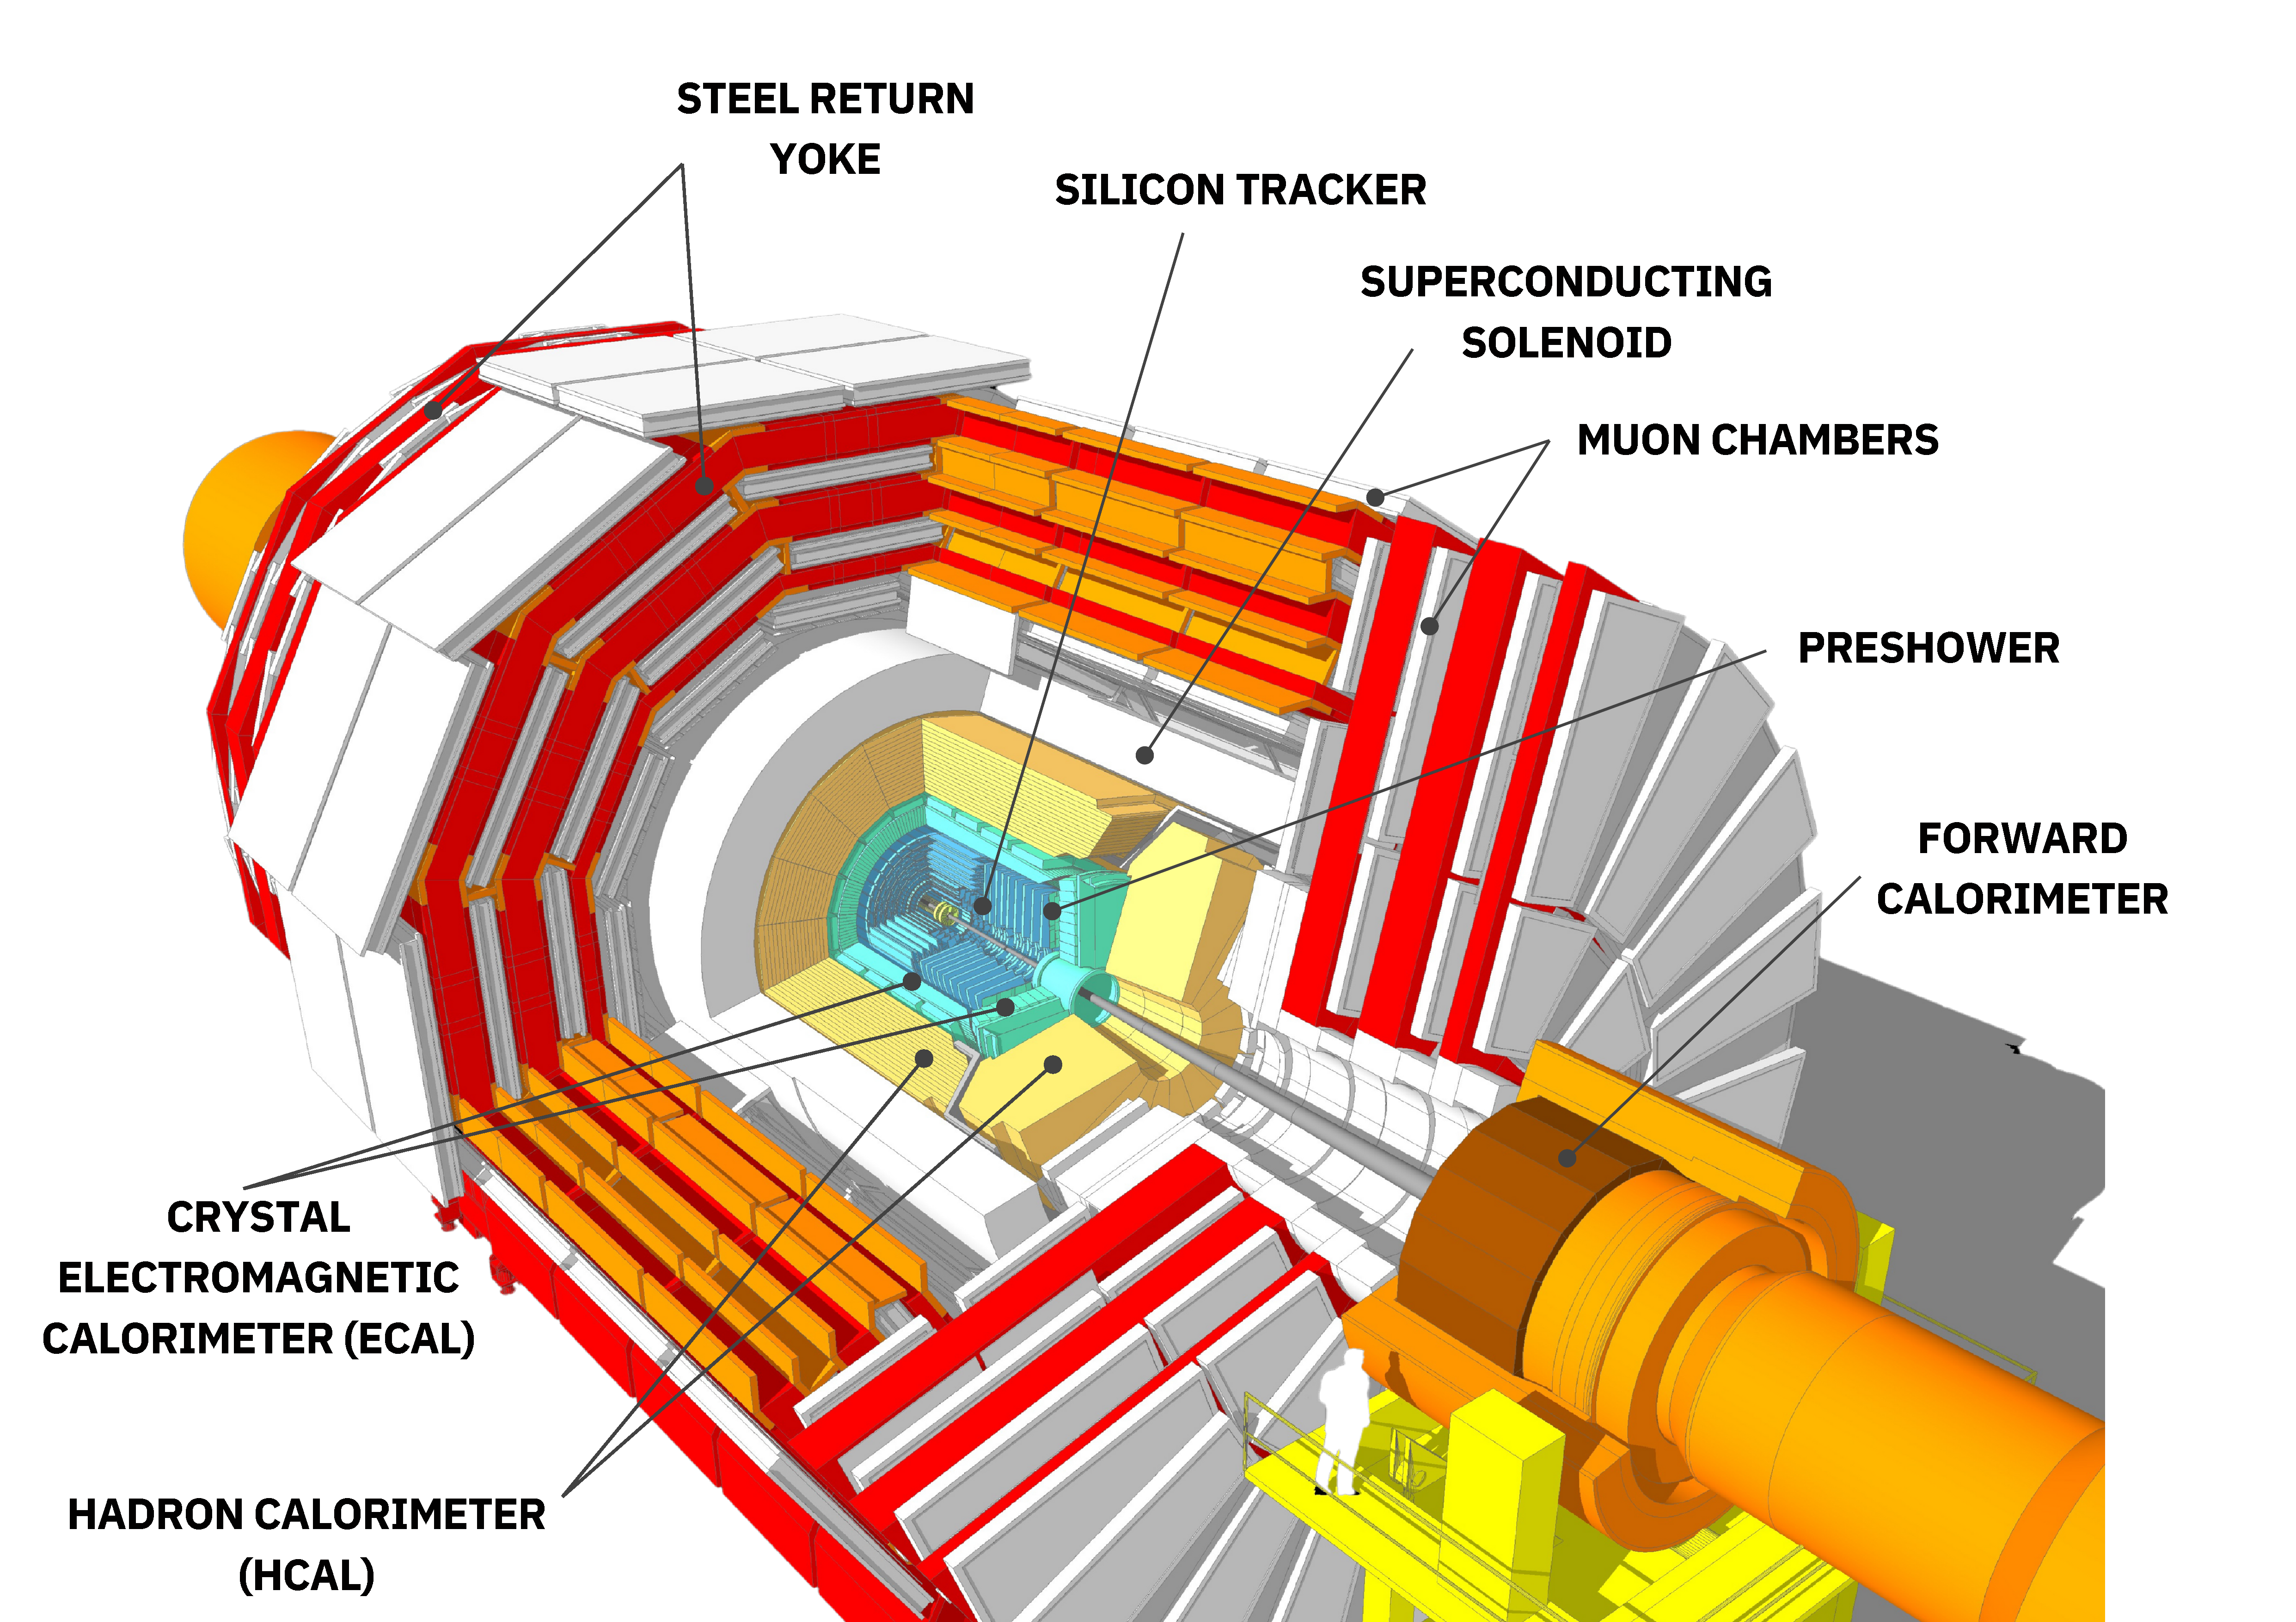
\includegraphics[width= 0.8\textwidth]{Figures/Chapter3/CMS_Detector.pdf}
\caption[Schematic drawing of the CMS detector]{Schematic drawing of the CMS detector. Figure taken from Ref.~\cite{CMS_Detector_Run3}.}
\label{Figure:Chapter3_CMS_schematic}
\end{figure}

\begin{figure}[h]
\centering
\includegraphics[width= 0.8\textwidth]{Figures/Chapter3/CMS_Detector_Slice.pdf}
\caption[Transverse slice of the CMS detector]{A transverse slice of the CMS detector displaying the individual subsystems and their response to different types of particles. Figure adjusted from Ref.~\cite{CMS_Detector_Slice}.}
\label{Figure:Chapter3_CMS_slice}
\end{figure}

\clearpage
\subsection{Co-ordinate system}
CMS adopts a right-handed Cartesian coordinate system centred at the nominal collision point. The $x$-axis points towards the centre of the LHC ring, and the $y$-axis points vertically upwards, while the $z$-axis points along the beam direction towards the Jura mountains, as illustrated in Fig.~\ref{Figure:Chapter3_CMS_CoordinateSystem}.

\begin{figure}[h]
\centering
\includegraphics[width= 0.8\textwidth]{Figures/Chapter3/CMS_CoordinateSystem.pdf}
\caption{The CMS detector coordinate system.}
\label{Figure:Chapter3_CMS_CoordinateSystem}
\end{figure}

In this system, the plane perpendicular to the beam axis, $x-y$ plane, is referred to as the \textit{transverse plane}, while the $z$-axis defines the \textit{longitudinal direction}. The \textit{azimuthal angle} $\phi \in [0,2\pi]$ is the angle with respect to the positive $x$-axis in the transverse plane, while the \textit{polar angle} $\theta \in [0,\pi]$ is with respect to the $z$-axis. Rather than using $\theta$ directly, it is common in collider physics to introduce \textit{pseudorapidity} ($\eta$), defined as

\begin{equation_pad}
    \eta = - \ln\left[\tan(\theta/2)\right]
\end{equation_pad}

A key property of this quantity is that the difference in pseudorapidity ($\Delta\eta$) between two vectors is invariant under Lorentz boosts along the longitudinal $z$-axis. This is convenient in hadron collider experiments, where the parton-parton centre-of-mass frame is often significantly boosted along the beam direction due to the variable momentum fractions carried by the incoming partons. Additionally, $\eta$ provides a nearly linear mapping of $\theta$ (shown in Fig.~\ref{Figure:Chapter3_Pseudorapidity}), facilitating a simple description of particle emission angles relative to the beam axis. This property allows for a natural segmentation of the detector into barrel and endcap regions based on $\eta$.

\begin{itemize} 
\item \textbf{Barrel region}: The central cylindrical region of the detector, located closest to the primary interaction point and optimised for particles emitted at large angles to the beamline ($\ie$ low $|\eta|$). 
\item \textbf{Endcap regions}: Located at either end of the barrel along the $z$-axis, designed to detect particles emitted at small angles with respect to the beamline ($\ie$ high $|\eta|$). 
\end{itemize}

\begin{figure}[h]
\centering
\includegraphics[width= 0.8\textwidth]{Figures/Chapter3/Pseudorapidity.pdf}
\caption{Illustration of the relationship between pseudorapidity ($\eta$) and polar angle ($\theta$).}
\label{Figure:Chapter3_Pseudorapidity}
\end{figure}

At the LHC, the initial momentum component of the system perpendicular to the beam axis is nearly zero because of the head-on nature of the beam. This kinematic quantity is referred to as the transverse momentum ($p_\mathrm{T}$) and is defined as:

\begin{equation_pad}
    p_\mathrm{T} = \sqrt{p_x^2 + p_y^2}
\end{equation_pad}

Transverse momentum is a central observable in collider physics. It provides a direct probe of hard interaction processes characterised by large momentum transfers. A complementary quantity to the transverse momentum is the missing transverse momentum ($E_\mathrm{T}^{\text{miss}}$), which is defined as the negative vector sum of the transverse momenta of all reconstructed particles in an event. This is a critical quantity serving as an estimator of the transverse momentum carried by non-interacting or undetected particles.

The radial distance from the beam axis is typically expressed as $r = \sqrt{x^2+y^2}$. Additionally, it is also convenient to express the distance metric ($\Delta R$) between two objects in a Lorentz-invariant way as:

\begin{equation_pad}
    \Delta R = \sqrt{(\Delta\eta)^2 + (\Delta \phi)^2}
\end{equation_pad}

This quantity is important in object reconstruction, as discussed in Section~\ref{Section:Chapter4}.%

\subsection{Magnet System}

As its name implies, CMS is defined by its central feature: the solenoid magnet. This critical component generates a very strong magnetic field that bends the trajectories of charged particles as they traverse the detector. This enables precise measurements of their momenta and electric charges. 

The \textbf{solenoid} spans $13\unit{m}$ in length and $6\unit{m}$ in diameter, capable of producing a magnetic field of up to $4\unit{T}$, but is currently operated at $3.8\unit{T}$ for enhanced long-term stability. The strong field ensures that low-momentum charged particles are sufficiently curved, confining them within the inner tracking system and aiding in precise momentum resolution. This not only improves tracking quality but also helps mitigate calorimeter noise by preventing soft particles from reaching the calorimeters.

Outside the solenoid, the muon detection system is embedded within segmented layers of iron, forming the \textbf{iron yoke}. This massive structure, weighing approximately $10,000\unit{t}$, serves two primary purposes: it returns about two-thirds of the magnetic flux generated inside the detector and provides structural support for the muon chambers. By returning the flux, the iron yoke significantly reduces the magnetic field outside the detector. This magnetic field configuration causes a ``\textit{double bending}'' of muon trajectories: first in one direction as muons pass through the inner silicon tracker, and then in the opposite direction as they traverse the muon chambers embedded in the iron yoke. This double bending significantly enhances the overall muon momentum resolution.

\subsection{Inner tracking system}
The CMS interaction point is surrounded by the innermost subdetector, the \textbf{silicon tracker}, which measures $5.8\unit{m}$ in length and $2.5\unit{m}$ in diameter~\cite{LHC_CMS,CMS_Detector_Run3}. The tracker plays a central role in reconstructing the trajectories of charged particles and in identifying both primary and secondary interaction vertices with high spatial precision.

At the LHC’s design luminosity, on the order of $10^3$ charged particles traverse the tracker volume per each $25\unit{ns}$ bunch crossing. To cope with the extreme occupancy, the tracker must combine high granularity with rapid signal readout. Furthermore, its proximity to the interaction point exposes it to a harsh radiation environment, necessitating the use of radiation-hard sensor technologies to preserve long-term performance.

To meet these demanding requirements, the CMS tracker employs \textit{silicon-based sensors}. However, these silicon sensors also require dedicated readout electronics and active cooling systems. These components contribute to the non-active material within the tracking volume, which must be carefully controlled. Excessive material leads to increased multiple scattering and energy loss, degrading momentum resolution and negatively impacting the performance of outer subdetectors such as the calorimeters.

As shown in Fig.~\ref{Figure:Chapter3_Tracker_MaterialBudget}, the material budget of the tracker is kept as low as possible, particularly in the central (low-$\eta$) region of the pixel detector, where precision tracking is most critical.

\begin{figure}[h]
    \centering
    % First row
    \begin{subfigure}[b]{0.49\textwidth}
        \centering
        \includegraphics[width=\textwidth]{Figures/Chapter3/Material_Budget1.pdf}
        \caption{}
    \end{subfigure}
    \begin{subfigure}[b]{0.49\textwidth}
        \centering
        \includegraphics[width=\textwidth]{Figures/Chapter3/Material_Budget2.pdf}
        \caption{}
    \end{subfigure}
\caption[Simulation of the CMS pixel detector material budget]{Simulation of the CMS pixel detector material budget as a function of $\eta$ in units of ($\textbf{a}$) radiation length and ($\textbf{b}$) hadronic interaction length for different detector components. Figure taken from Ref.~\cite{TrackerMaterialBudget_Pixel}.}
\label{Figure:Chapter3_Tracker_MaterialBudget}
\end{figure}

\newpage
\subsubsection{Pixel Detector}

The innermost component of the CMS tracking system is the \textbf{silicon pixel detector}. The original pixel detector~\cite{LHC_CMS}, installed in 2008, was designed to operate for up to ten years under the LHC’s nominal instantaneous luminosity of $1 \times 10^{34}\unit{cm}^{-2}\unit{s}^{-1}$, with the capacity to handle up to 25 PU interactions ber bunch crossing. However, even during Run-1, the LHC exceeded its design luminosity, exposing the pixel detector to increased radiation levels and causing rising readout inefficiencies. To maintain high tracking efficiency under upgraded luminosity conditions of up to $2 \times 10^{34}~\unit{cm}^{-2}\unit{s}^{-1}$ and PU levels of 50 or more, the CMS pixel detector underwent a major upgrade in 2017, referred to as the Phase-1 upgrade~\cite{CMS_Detector_Run3, CMS_Tracker_Phase1_Upgrade,CMS_Tracker_Phase1_Upgrade_2}. This upgrade introduced a more granular and radiation-tolerant detector layout, featuring four barrel layers and three endcap disks.

The \textbf{\ac{BPIX}} detector consists of four concentric cylindrical layers (L1-L4) positioned at radii of 29, 68, 109, and 160$\unit{mm}$ from the beamline. A total of 1,184 sensor modules are deployed in the barrel region. Each module contains a silicon sensor segmented into $160 \times 416$ individual pixels with a pitch of $100 \times 150\unit{\mu m}^2$, enabling high-resolution hit detection. Compared to the original pixel detector, the innermost layer (L1) was also moved closer to the interaction point by reducing the CMS beam pipe radius from 30 to 23$\unit{mm}$ in 2014. 

The \textbf{\ac{FPIX}} detector complements the barrel coverage by extending tracking capabilities in the forward region. It comprises three endcap disks on each side of the detector, located at distances of 291, 396, and 516$\unit{mm}$ from the interaction point. The forward region is equipped with 672 pixel modules, featuring the same fine segmentation and pixel pitch as the barrel modules. Together, the BPIX and FPIX systems provide approximately 124 million readout channels, ensuring precise tracking throughout the detector’s angular coverage.

The Phase-1 upgrade of the CMS pixel detector introduced significant improvements in geometry and coverage, as illustrated in Fig.~\ref{Figure:Chapter3_Pixel_Upgrade}. Additionally, substantial gains were also achieved in spatial resolution and tracking performance. The position resolution reaches approximately $11\unit{\mu m}$ in the $r-\phi$ direction and $24\unit{\mu m}$ in the $z$ direction for BPIX L3. Somewhat worse resolutions are observed in the innermost barrel layers due to higher radiation damage. For FPIX, the corresponding resolutions are about $12\unit{\mu m}$ ($r$) and $21\unit{\mu m}$ ($z$). 

\begin{figure}[h]
\centering
\includegraphics[width=1\textwidth]{Figures/Chapter3/CMS_Pixel_Upgrade.pdf}
\caption[Longitudinal view of CMS pixel detector before and after Phase-1 Upgrade]{Longitudinal view of CMS pixel detector comparing its structure before (lower part) and after (upper part) the Phase-1 Upgrade. Figure taken from Ref.~\cite{CMS_Detector_Run3}.}
\label{Figure:Chapter3_Pixel_Upgrade}
\end{figure}

The improved granularity and four-hit coverage introduced in the Phase-1 pixel detector enable robust three-dimensional reconstruction of charged particle trajectories, which is essential for precise identification of both primary and secondary vertices. Consequently, these tracking enhancements lead to improved vertex reconstruction performance. As shown in Fig.~\ref{Figure:Chapter3_Pixel_Vertex_Resolution}, the transverse ($x,y$) vertex resolution achieved with the Phase-1 detector is significantly better than that of the Phase-0 detector.

\begin{figure}[h]
    \centering
    % First row
    \begin{subfigure}[b]{0.49\textwidth}
        \centering
        \includegraphics[width=\textwidth]{Figures/Chapter3/Pixel_Vertex_XY_Resolution.pdf}
        \caption{}
    \end{subfigure}
    \begin{subfigure}[b]{0.49\textwidth}
        \centering
        \includegraphics[width=\textwidth]{Figures/Chapter3/Pixel_Vertex_Z_Resolution.pdf}
        \caption{}
    \end{subfigure}
\caption[Vertex resolution comparison between Phase-0 and Phase-1 pixel detectors]{Comparison of the simulated CMS vertex resolution between the Phase-0 and Phase-1 pixel detectors as a function of the number of tracks used in the vertex fit. \textbf{(a)} Transverse ($x,y$) vertex resolution. \textbf{(b)} Longitudinal ($z$) vertex resolution. Figures taken from Ref.~\cite{Pixel_Vertex_Performance}.}

\label{Figure:Chapter3_Pixel_Vertex_Resolution}
\end{figure}


\subsubsection{Silicon Strip Tracker}
Surrounding the pixel detector is the \textbf{\ac{SST}}, illustrated in Fig.~\ref{Figure:Chapter3_Tracker_Geometry}. In the outer tracking region, lower particle occupancy allows the use of silicon strips instead of pixels, relaxing granularity requirements and enabling larger sensor elements. The SST covers an active area of approximately $198\unit{m}^2$ and contains 9.3 million silicon micro-strips distributed across 15,148 detector modules. It is composed of four main subsystems: the \ac{TIB}, \ac{TID}, \ac{TOB}, and \ac{TEC}.

\begin{figure}[h]
\centering
\includegraphics[width=1\textwidth]{Figures/Chapter3/Phase1_Tracker.pdf}
\caption[Schematic of CMS inner tracking system in the $(r-z)$ plane]{Schematic view of one-quarter of the CMS inner tracking system in the $(r-z)$ plane. The pixel detector is depicted in green, located close to the beamline. Single-sided and double-sided strip modules are depicted as red and blue segments, respectively. Figure adjusted from Ref.~\cite{CMS_Detector_Run3}.}
\label{Figure:Chapter3_Tracker_Geometry}
\end{figure}

The \textbf{TIB} is made up of four cylindrical barrel layers located just outside the pixel detector. It provides precise tracking in the central pseudorapidity region and extends out to a radius of $r < 550\unit{mm}$. The strip pitch in the TIB ranges from approximately $80-120\unit{\mu m}$, depending on the layer and module type. To ensure complete coverage and continuity in tracking performance, the TIB is complemented by the \textbf{TID}, which consists of three disk-shaped structures at each end of the TIB, extending the longitudinal reach to $|z| < 1180\unit{mm}$. The TID uses similar strip pitches, typically around $100-141\unit{\mu m}$. Together, the TIB and TID form the inner part of the strip tracking system, which is crucial for linking tracks from the pixel detector to the outer layers.

The \textbf{TOB} extends the radial coverage beyond the inner systems, occupying the region $r > 550\unit{mm}$. It consists of six cylindrical barrel layers, providing high-precision measurements over a larger area with longer strip modules. The strip pitch in the TOB is coarser than in the inner systems, with a pitch of approximately $183\unit{\mu m}$ in the inner TOB layers and $122\unit{\mu m}$ in the outer layers. The TOB ensures efficient momentum resolution and track reconstruction for particles passing through the outer barrel region, especially those with lower transverse momentum.

The \textbf{TEC} completes the strip tracker by covering the forward pseudorapidity regions. Each TEC consists of nine disks positioned between $1240 < |z| < 2820\unit{mm}$ on either side of the detector. These disks contain up to seven concentric rings of silicon strip modules, which are carefully arranged to maintain uniform tracking performance and coverage up to $|\eta| \simeq 2.5$. The strip pitch in the TEC varies across the radial zones of the disks and generally ranges from $97-184\unit{\mu m}$.

In the barrel sections, the modules are oriented to measure the radial $r\text{-}\phi$ coordinates. Conversely, in the TID and TEC sections, they are primarily aligned to measure $\phi\text{-}z$ coordinates.

In the innermost two layers of the TIB and TOB, the first two rings of the TID, and rings 1, 2, and 5 of the TEC, double-sided modules are deployed. These consist of two single-sided sensors mounted back-to-back with a stereo angle of $100\unit{mrad}$. The combination of their signals enables three-dimensional hit reconstruction, providing an additional measurement of the $z$ coordinate in the barrel and the $r$ coordinate in the disk regions.

\subsection{Electromagnetic calorimeter}

As outlined by the LHC physics requirements in Section~\ref{Section:Chapter3_CMS_Detector_Introduction}, precise reconstruction of electromagnetic particles and robust suppression of background processes ($\pi^0 \to \gamma \gamma$) are essential for CMS. The CMS \textbf{ECAL}~\cite{LHC_CMS,CMS_Detector_Run3,CMS_ECAL_Performance_Run2} is designed to meet these demands, providing high-resolution energy measurements for electrons and photons. It is composed of three main subsystems: a central barrel calorimeter, two endcap calorimeters, and a preshower detector situated in front of the endcaps.

The ECAL is a hermetic homogeneous calorimeter consisting of 61,200 lead tungstate (PbWO$_4$) crystals mounted in the central \textbf{barrel} part. These crystals are arranged in a quasi-projective geometry, with their axes slightly tilted ($3^\circ$) relative to the line from the nominal interaction point. This geometry minimises gaps in the detector and reduces the probability of particles passing through the cracks between crystals. The barrel region covers the pseudorapidity range $|\eta| < 1.479$ and features a 360-fold segmentation in $\phi$ and a ($2 \times 85$)-fold segmentation in $\eta$. Each barrel crystal has a front face cross-section of $22 \times 22\unit{mm}^2$ and a length corresponding to $25.8~X_0$, ensuring that most electromagnetic showers are well-contained within a few crystals.

The \textbf{endcap} region complements the barrel coverage, extending the ECAL acceptance to $1.479 < |\eta| < 3.0$ with 7,324 crystals in each of the two endcaps. These crystals are larger in cross-section ($28.62 \times 28.62\unit{mm}^2$) and slightly shorter in length ($24.7 X_0$) compared to those in the barrel. As in the barrel, the PbWO$_4$ crystals are precisely arranged to maintain fine granularity.

The \textbf{Preshower} system is installed in front of the endcaps, covering a fiducial region of $1.653 < |\eta| < 2.6$. It is designed explicitly for $\pi^0$ rejection by distinguishing between closely spaced photon pairs from $\pi^0 \to \gamma \gamma$ decays. The PS is a $20\unit{cm}$ ($3X_0$) thick sampling calorimeter composed of two alternating layers of lead to initiate electromagnetic showers and silicon strip sensors to measure the deposited energy and transverse shower profiles.

The selection of PbWO$_4$ crystals for all ECAL regions is motivated by their desirable properties: high density ($8.28\unit{gcm}^{-3}$), short radiation length ($0.89\unit{cm}$), and small Moli\`ere radius ($2.2\unit{cm}$). This allows for a compact and granular calorimeter design. Additionally, these crystals emit about 80\% of their scintillation light within $25\unit{ns}$, matching the LHC bunch crossing time and enabling efficient energy collection within a single event window.

A crucial component of the CMS ECAL is the photodetectors, which convert the scintillation light produced in the PbWO$_4$ crystals into electrical signals. Due to the relatively low light yield of these crystals, the photodetectors must provide internal amplification. They must also exhibit a fast response, high radiation tolerance, and compatibility with the strong longitudinal magnetic field of the CMS solenoid ($3.8-4\unit{T}$). \textit{\ac{APDs})} and \textit{\ac{VPTs}} are employed in the barrel and endcap regions, respectively. Although VPTs offer lower quantum efficiency and gain compared to APDs, their exceptional radiation hardness and ability to operate in high-field environments make them well-suited for the endcap configuration.

As shown in Figures~\ref{Figure:Chapter3_CMS_schematic}-\ref{Figure:Chapter3_CMS_slice}, the ECAL is positioned outside the inner tracking system and in front of the hadronic calorimeter. A schematic of the CMS ECAL is shown in Fig.~\ref{Figure:Chapter3_CMS_ECAL}.

\begin{figure}[h]
\centering
\includegraphics[width= .85\textwidth]{Figures/Chapter3/CMS_ECAL.pdf}
\caption[Schematic view of the CMS ECAL subdetector]{Schematic view of the CMS ECAL subdetector. Figure taken from Ref.~\cite{LHC_CMS}.}
\label{Figure:Chapter3_CMS_ECAL}
\end{figure}
\newpage
The energy resolution of the ECAL is parametrised as a function of the incident particle energy $E$ as:

\begin{equation_pad}
    \left(\frac{\sigma}{E}\right)^2 =  \underbrace{\left(\frac{S}{\sqrt{E}}\right)^2}_{\text{Stochastic}} +  \underbrace{\left(\frac{N}{E}\right)^2}_{\text{Noise}} +  \underbrace{C^2}_{\text{Constant}}
\end{equation_pad}

Each term reflects a different contribution to the resolution: the stochastic term accounts for statistical fluctuations in lateral shower containment and photon yield; the noise term reflects electronic noise and PU; and the constant term arises from detector non-uniformities ($\eg$ longitudinal response) and calibration uncertainties. During an electron test beam in 2014~\cite{ECAL_TestBeam}, the ECAL demonstrated excellent energy resolution, consistent with the design specifications:

\begin{equation_pad}
    \left(\frac{\sigma}{E}\right)^2 =  \underbrace{\left(\frac{2.8\%}{\sqrt{E}}\right)^2}_{\text{Stochastic}} +  \underbrace{\left(\frac{0.12}{E}\right)^2}_{\text{Noise}} +  \underbrace{(0.30\%)^2}_{\text{Constant}}
\end{equation_pad}

\subsection{Hadronic calorimeter}
To complete the calorimetric measurement and ensure accurate reconstruction of hadronic jets and \ac{MET}, the CMS detector employs a dedicated HCAL system. Positioned outside the ECAL, the HCAL is a sampling calorimeter designed to detect strongly interacting particles and spans the pseudorapidity range $|\eta| < 5.2$~\cite{LHC_CMS,CMS_Detector_Run3}. The HCAL comprises four distinct components: the \ac{HB}, \ac{HE}, \ac{HO}, and \ac{HF} calorimeters, as shown in Fig.~\ref{Figure:Chapter3_CMS_HCAL}.

\begin{figure}[h]
\centering
\includegraphics[width= 1.0\textwidth]{Figures/Chapter3/CMS_HCAL.pdf}
\caption[Schematic of CMS detector highlighting HCAL sub-detectors]{A schematic view of one-quarter of the CMS detector with the locations of the HB, HO, HE and HF sub-detectors of the HCAL being shown. Figure adjusted from Ref.~\cite{LHC_CMS}.}
\label{Figure:Chapter3_CMS_HCAL}
\end{figure}

The \textbf{HB} and \textbf{HE} subdetectors are located within the bore of the magnet, covering the pseudorapidity regions $|\eta| < 1.3$ and $1.3 < |\eta| < 3.0$, respectively. They are constructed using alternating layers of brass absorber plates and plastic scintillators. Brass is used due to its short nuclear interaction length and non-magnetic nature, the latter being essential for operation within the CMS solenoid. The HB has a minimum absorber thickness of 5.82 interaction lengths ($\lambda_0$), which increases with polar angle as ($1/\sin\theta$) to approximately 10.6~$\lambda_0$ at $|\eta| = 1.3$. In the \textbf{HE}, 79$\unit{mm}$ thick brass plates interleaved with 9$\unit{mm}$ scintillator gaps provide a total depth of around 10$\lambda_0$, including the contribution from the electromagnetic crystals in front. The calorimeter segmentation is $\Delta\eta \times \Delta\phi = 0.087 \times 0.087$ for $|\eta| < 1.6$, and approximately $0.17 \times 0.17$ for $|\eta| \geq 1.6$. Charged particles from hadronic showers deposit energy in the scintillator tiles, producing scintillation light that is collected by wavelength-shifting fibres and read out using hybrid photodiodes.

Due to the solenoid magnet, the HB is radially restricted, constraining the total amount of material which can be inserted to absorb hadronic showers. As a result, the combined stopping power of the EB and HB does not provide sufficient containment of the hadronic showers. The \textbf{HO} subdetector is used as a tail catcher outside of the solenoid, aiming to ensure adequate sampling depth for $|\eta| < 1.3$. The HO employs the same active scintillator as the HB, while also utilising the solenoid as an additional absorber, extending the minimum depth to 11.8$\lambda_0$. This extended sampling is crucial for identifying and measuring the energy of late-starting or highly penetrating showers.

Beyond $|\eta| < 3.0$, the \textbf{HF} sub-detector extends the pseudorapidity coverage of the CMS HCAL to $|\eta| < 5.2$, and is located at $\pm 11.2\unit{m}$ from the interaction point. Its design posed significant challenges due to the extremely harsh radiation environment in the forward region, where particle fluxes reach unprecedented levels. To ensure long-term durability, the HF was constructed using highly radiation-resistant materials. Quartz fibres were chosen as the active medium, embedded within a steel absorber composed of 5$\unit{mm}$ thick grooved plates into which the fibres are inserted. The HF subdetector is segmented longitudinally into two readout depths: one set of fibres spans the entire 165$\unit{cm}$ depth of the absorber (approximately 10~$\lambda_0$), while the other begins at a depth of 22$\unit{cm}$. By reading out these fibre sets independently, the HF can discriminate between electromagnetic showers, which deposit a large fraction of their energy in the first $22\unit{cm}$ and hadronic showers, which deposit their energy more uniformly across the full depth. When charged particles pass through the quartz fibres, they produce Cherenkov light, which is then collected and transmitted to photomultiplier tubes. The use of Cherenkov light makes the HF relatively insensitive to low-energy particles and neutral backgrounds, such as neutrons or secondary products from activated radionuclides, helping to reduce noise in this high-radiation environment.

When combining information from the inner tracking system with measurements from the calorimeters, the jet energy resolution typically reaches 15\% at $10\unit{GeV}$, 8\% at $100\unit{GeV}$, and 4\% at $1\unit{TeV}$. In comparison, using only the ECAL and HCAL calorimeters yields resolutions of approximately 40\%, 12\%, and 5\% at the same energies, respectively~\cite{CMS_HCAL_EnergyResolution}.

\subsection{Muon system}
To satisfy the LHC’s stringent performance goals for muon reconstruction, CMS employs a dedicated muon tracking system~\cite{LHC_CMS,CMS_Muon_System_Performance} positioned furthest from the interaction point. The system serves three primary functions: muon identification, momentum measurement, and triggering. These are made possible by the strong solenoidal magnetic field and the iron return yoke, which acts as a hadron absorber.  CMS employs three complementary gaseous particle detector technologies for detecting muons.  

In the barrel region, where muon rates and neutron-induced backgrounds are relatively low, the $3.8–4\unit{T}$ magnetic field is uniform and largely confined within the iron yoke. \textbf{\ac{DTs}} are used here, providing coverage in the pseudorapidity region $|\eta| < 1.2$. These are organised into four stations interspersed among the layers of the flux return plates. The first three stations are further subdivided into eight chambers, four measuring the muon coordinate in the $r-–\phi$ bending plane and four providing a measurement in the $z$ direction. Conversely, the capabilities of the fourth muon station are restricted to $r–-\phi$ measurements. Each DT chamber consists of rectangular drift cells containing a central anode wire. The cells are filled with a gas mixture of argon and carbon dioxide, which enables efficient ionisation and drift of electrons toward the wire for signal detection. 

In contrast to the barrel region, the endcaps are subjected to higher muon rates and background levels. The magnetic field in this region is both strong and non-uniform, necessitating a finely segmented detector system that is radiation-resistant and capable of fast response times. To meet these demands, CMS employs \textbf{\ac{CSCs}} in the region $0.9 < |\eta|<2.4$. Each CSC is a multi-layered gaseous detector consisting of six planes of anode wires interleaved with seven cathode layers. In both endcaps, the chambers are arranged into four stations placed perpendicular to the beam line and embedded between the layers of the iron yoke. The cathode strips extend radially outward from the beam axis, providing precise position measurements in the $r-\phi$ plane. The anode wires, oriented roughly perpendicular to the strips, deliver additional spatial information in $\eta$ and enable timing measurements relative to the beam crossing. This six-layer configuration enhances pattern recognition, improving the rejection of spurious hits from background sources and allowing for efficient correlation with hits from other stations and with tracks reconstructed in the inner tracker.

The DT and CSC systems are complemented by the \textbf{\ac{RPC}} system in the pseudorapidity region $|\eta| < 1.6$. RPCs are double-gap chambers featuring anode and cathode plates separated by gas. Compared to DTs and CSCs, RPCs exhibit lower granularity; however, they offer a faster response and good time resolution. These characteristics make them particularly well-suited for use as trigger detectors. As such, they are especially valuable in scenarios where the DT and CSC systems may struggle to cope with PU-induced background. Additionally, RPCs contribute to resolving ambiguities when reconstructing tracks from multiple hits within a chamber, further enhancing the overall performance of the muon detection system.

A schematic illustration of the CMS muon detection system is shown in Fig.~\ref{Figure:Chapter3_CMS_Muon_System}, highlighting the arrangement of the DT, CSC, and RPC subdetectors within the return yoke. Owing to its design, the CMS muon system achieves a reconstruction and identification efficiency exceeding 95\% for muons with energies above a few $\unit{GeV}$. The momentum resolution varies between 1\% and 6\% for transverse momenta below $100\unit{GeV}$, and remains better than 10\% up to $1\unit{TeV}$~\cite{CMS_Muon_System_Performance_2}. Furthermore, the system reliably determines the muon charge sign for transverse momenta up to $1\unit{TeV}$.


\begin{figure}[h]
\centering
\includegraphics[width= 1.0\textwidth]{Figures/Chapter3/CMS_Muon_System.pdf}
\caption[Schematic of CMS muon detection system]{Schematic illustration of one quarter of the CMS detector, highlighting the muon detection system. The DT stations are labelled as MB (Muon Barrel), while the CSCs are labelled as ME (Muon Endcap). The RPCs are denoted as RB in the barrel region and RE in the endcap region. Figure taken from Ref.~\cite{CMS_Muon_System_Performance}.}
\label{Figure:Chapter3_CMS_Muon_System}
\end{figure}

\subsection{Trigger system}

At the LHC interaction points, proton bunches cross every $25\unit{ns}$, resulting in a nominal bunch crossing frequency of $40\unit{MHz}$. Additionally, each bunch crossing can yield up to more than 50~PU interactions corresponding to an aggregate rate of individual proton-proton interactions surpassing $1\unit{GHz}$. Recording all of these collisions is not feasible nor necessary, as only a small fraction contains events of interest to the CMS physics programme. To select the most interesting events, CMS employs a dedicated two-level trigger system~\cite{CMS_Trigger} consisting of the \textbf{\ac{L1} trigger} and the \textbf{\ac{HLT}}.

As the name suggests, the \textbf{L1 trigger} is the first level of the CMS trigger system, implemented as a hardware-based trigger on custom-built Field Programmable Gate Arrays with a fixed latency of $4\unit{\mu s}$. CMS relies on this system to rapidly determine whether an event should be tentatively accepted or rejected based on calorimeter energy deposits and muon detector hits. The L1 decision chain comprises three primary subsystems: the L1 calorimeter system, the L1 muon trigger system and the global trigger (GT), as shown in Fig.~\ref{Figure:Chapter3_CMS_L1_Trigger}.

\begin{figure}[h]
\centering
\includegraphics[width= 1.0\textwidth]{Figures/Chapter3/CMS_L1_Trigger.pdf}
\caption[Schematic of the CMS L1 trigger workflow]{Schematic of the CMS L1 trigger workflow. Figure reproduced from Ref.~\cite{CMS_L1_Trigger}.}
\label{Figure:Chapter3_CMS_L1_Trigger}
\end{figure}

The \textbf{L1 calorimeter trigger system} is organised into two processing layers. Layer-1 (\textit{Calo Trigger Layer 1}) receives trigger primitives (energy deposits) from the ECAL and the HCAL, performs initial calibrations, and sorts local energy deposits. Layer-2 (\textit{Calo Trigger Layer 2}) processes the calibrated information to reconstruct and further calibrate high-level physics objects such as electrons, photons, jets, taus, and MET. Simultaneously, hits from the three muon subsystems are processed by the first stage of the \textbf{L1 muon trigger system} (\textit{Muon Tracking-Finder Layer}). At this stage, track finding is performed by combining hits within sectors in $\phi$ and $\eta$. The reconstructed track candidates are then forwarded to the \textit{Sorting and Merging Layer}, where information from the $\phi$ sectors is consolidated. The output, along with the calorimeter information required to compute isolation, is passed to the global muon trigger, where a sorted list of muon candidates for the entire detector is produced. Finally, the \textbf{global trigger} integrates the information from both the L1 calorimeter and muon trigger systems, enabling it to make a decision on the fate of the event. This allows for the event rate to be reduced from $40\unit{MHz}$ to $100\unit{kHz}$.

The \textbf{HLT} system is the second stage of the CMS trigger architecture. It is a software-based trigger that runs on a processor farm composed of commercial CPUs. In contrast to the hardware-based L1 trigger, the HLT utilises full-resolution data from the CMS detector and applies offline-quality reconstruction algorithms for more refined event selection. The primary objective of the HLT is to further reduce the event rate to about $1\unit{kHz}$ for permanent storage and offline analysis. 

Rather than operating with fixed latency, the HLT processes events asynchronously, scaling with available CPU resources. Its workflow is organised into HLT paths, each consisting of a predefined sequence of algorithmic steps that reconstruct and select physics objects. These paths are structured to increase in complexity, precision, and physics sophistication. To optimise computational efficiency, initial selections use fast information from the calorimeters and muon detectors, while CPU-intensive tracking is applied only to events that pass these preliminary filters. 

Events accepted by the HLT are handed off to the storage manager, which writes them temporarily to local disk. They are then transferred to the CMS Tier‑0 computing centre for offline reconstruction and long‑term archival.



\setcounter{mtc}{4}
\chapter{Object reconstruction}
\chaptermark{Object reconstruction}  
\thispagestyle{plain}  % First page has default style
\pagestyle{chapterpages}
\label{Section:Chapter4}
\minitoc

This chapter presents the reconstruction and identification of physics objects in the CMS detector, which is foundational to all analyses performed in this thesis. In particular, $\PGt$ lepton reconstruction is a central focus. This is a particularly challenging task due to its short lifetime and complex decay modes, which can involve a mix of charged and neutral hadrons, electrons, muons, and undetectable neutrinos. Therefore, excellent performance of multiple reconstruction components is required, including charged-particle tracking, electromagnetic and hadronic calorimetry, muon identification, and displaced secondary vertexing.

However, operating in a high-multiplicity environment introduces additional challenges for the reconstruction and identification of physics objects. There is no guarantee that a reconstructed particle corresponds to a genuine physics object; such cases are referred to as \textit{misidentified} or \textit{``fake'' objects}. For example, jets initiated by quarks or gluons can sometimes be misidentified as hadronic $\PGt$ decays; leptons originating from heavy-flavour decays within jets may mimic prompt electrons or muons; and, conversely, muons and electrons can occasionally be misidentified as jets. To mitigate these effects, object identification algorithms incorporate \textit{multivariate discriminants} and \textit{\acp{WP}} that are tuned to balance efficiency and misidentification rates. However, in some cases, these strategies only partially suppress such backgrounds.

A more complete and accurate event description is achieved by correlating information from all layers of the CMS detector to reconstruct and identify individual particles. This integrated methodology is known as \textbf{\ac{PF}} reconstruction. The implementation of this approach within CMS is detailed in this chapter.

\section{Reconstruction of Particle Flow detector elements}
\label{Section:Chapter4_Reconstruction_of_PF_elements}
\subsection{Track reconstruction}

The first stage of the reconstruction process, known as \textbf{local reconstruction}~\cite{CMS_TrackerPerformance_2014,CMS_Track_Reconstruction_Run2_3}, involves clustering zero-suppressed signals above predefined thresholds in the tracker sensors to form hits, referred to as \textit{clusters}. For each cluster, both the position and its associated uncertainty are estimated within a local coordinate system defined by the sensor geometry. These locally reconstructed hits form the basis for the subsequent \textbf{global reconstruction}~\cite{CMS_TrackerPerformance_2014,CMS_Track_Reconstruction_Run2_3} of particle trajectories.

Global track reconstruction is facilitated by the \textbf{\ac{CTF}} algorithm~\cite{CMS_TrackerPerformance_2014,CMS_Track_Reconstruction_Run2_3}, an adaptation of the combinatorial \textit{\ac{KF}}~\cite{KF_1,KF_2,KF_3}\footnote{KF~\cite{KF_4} is recursive algorithm that uses a series of measurements over time to estimate the state of a system. This is done by estimating a joint probability distribution over the variables of interest at each time step.} approach. This adaptation enables pattern recognition and track fitting to be performed within a unified framework, allowing hits to be incrementally added and track parameters to be continuously updated in a process known as \textbf{iterative tracking}. A single iteration of the CTF algorithm proceeds in four steps:

\begin{enumerate}
    \item \textbf{Seed generation}: Initial track candidates are formed using a small number of hits (typically two or three) in the innermost layers of the tracker. Each \textit{seed} provides an initial estimate of the particle's trajectory parameters, such as position, direction, and momentum, as well as their associated uncertainties. 
    \item \textbf{Track finding}: Seed trajectories are extrapolated along the expected trajectory of a charged particle using a Kalman Filter (KF). At each detector layer, additional hits along the expected flight path are identified and associated with the track candidate; the trajectory parameters are then updated accordingly. This process is repeated iteratively until the outermost layer of the detector is reached, gradually building complete track candidates from the initial seeds.
    \item \textbf{Track fitting}: The final trajectory is refitted iteratively to improve the estimate of the track parameters. This is done using a combination of a KF and a smoother, incorporating all available hit information.
    \item \textbf{Track selection}: Tracks are required to pass a set of quality flags.
\end{enumerate}

The \textbf{iterative tracking} procedure in CMS is performed in successive iterations, each designed to target different classes of tracks, as summarised in Table~\ref{Table:Chapter4_IterativeTrackingSeeds}. The initial iterations target tracks that are the easiest to find (\eg high $p_\mathrm{T}$ tracks, and tracks produced near the primary interaction point). After each iteration, the combinatorial complexity is reduced by removing hits associated with tracks. This enables later iterations to target more challenging classes of tracks (\eg low $p_\mathrm{T}$ tracks, and tracks displaced from the interaction point). 

\begin{table}[h]
\centering
\renewcommand{\arraystretch}{1.5} % Increase row height
\arrayrulecolor{black} % Ensure outer borders are black
\begin{tabular}{|c|l|l|l|}
\hline
Iteration & Name & Seeding & Targeted Tracks \\ \hline \hline
1         & InitialStep              & pixel triplets              & prompt, high $p_\mathrm{T}$                     \\
\arrayrulecolor{lightgray} \hline
2         & DetachedTriplet          & pixel triplets              & b hadron decays, R $\leq 5\unit{cm}$      \\
\arrayrulecolor{lightgray} \hline
3         & LowPtTriplet             & pixel triplets              & prompt, low $p_\mathrm{T}$                      \\
\arrayrulecolor{lightgray} \hline
4         & PixelPair                & pixel pairs                 & recover high $p_\mathrm{T}$                     \\
\arrayrulecolor{lightgray} \hline
5         & MixedTriplet             & pixel+strip triplets        & displaced, R $\leq 7\unit{cm}$                \\
\arrayrulecolor{lightgray} \hline
6         & PixelLess                & strip triplets/pairs        & very displaced, R $\leq 25\unit{cm}$          \\
\arrayrulecolor{lightgray} \hline
7         & TobTec                   & strip triplets/pairs        & very displaced, R $\leq 60\unit{cm}$          \\
\arrayrulecolor{lightgray} \hline
8         & JetCoreRegional          & pixel+strip pairs           & inside high $p_\mathrm{T}$ jets                 \\
\arrayrulecolor{lightgray} \hline
9         & MuonSeededInOut          & muon-tagged tracks          & muons                               \\
\arrayrulecolor{lightgray} \hline
10        & MuonSeededOutIn          & muon detectors              & muons                               \\
\arrayrulecolor{black} \hline
\end{tabular}
\caption[Summary of iterative tracking steps in CMS]{Summary of the iterations used in the CMS iterative tracking algorithm. Table taken from Ref.~\cite{ParticleFlow}.}
\label{Table:Chapter4_IterativeTrackingSeeds}
\end{table}

\subsection{Vertex reconstruction}

The primary goal of the CMS vertex reconstruction~\cite{CMS_TrackerPerformance_2014} is to determine the positions and associated uncertainties of all pp interaction vertices in an event, including both the \textbf{\ac{PV}} (associated with the \textit{``signal'' interaction}) and any additional vertices originating from PU collisions, using all available reconstructed tracks. The reconstruction process is performed in three main steps: 

\begin{enumerate}
    \item \textbf{Track selection}: Tracks consistent with originating promptly near the centre of the luminous region (referred to as the beam spot) are selected. This selection is based on applying quality requirements to the tracks, such as cuts on the transverse impact parameter\footnote{The impact parameter is defined as the distance of closest approach of a charged particle’s trajectory to the PV} significance relative to the beam spot and minimum numbers of associated pixel and strip hits.
    \item \textbf{Track clustering}: Tracks are clustered into groups that appear to be originating from the same vertex. This clustering is performed based on their z-coordinate at the point of closest approach to the beam spot using a \textit{deterministic annealing algorithm}~\cite{DeterministicAnnealing}.
    \item \textbf{Vertex fitting}: Candidate vertices composed of at least two tracks are fitted using an \textit{adaptive vertex fitter}~\cite{VertexFitting_2006,VertexFitting_2007} to determine the best estimate of the vertex parameters. These parameters include the $x$, $y$, and $z$ positions, the associated covariance matrix, and indicators of fit quality. Additionally, the adaptive fit assigns a weight between 0 and 1 to each track, reflecting the probability that the track is genuinely associated with the vertex.
\end{enumerate}

Once all the vertices are reconstructed, a collection is formed, which is ordered by the quadratic sum of the transverse track momenta associated with each vertex, $\sum_{\text{tracks}} p_{\mathrm{T}}^2$. The vertex with the largest sum is assumed to most likely correspond to the vertex of the hard scattering process~\cite{ParticleFlow}. The efficiency to correctly identify the PV when at least three tracks are associated is close to 100\%~\cite{CMS_TrackerPerformance_2014}. The resolution of the PV position, particularly in the $x$ and $z$ coordinates, has been measured using $\sqrt{s} = 13\ \mathrm{TeV}$ collision data~\cite{PrimaryVertex_Resolution} and is found to improve rapidly as the summed $p_{\mathrm{T}}$ of the associated tracks increases, as shown in Fig.~\ref{Figure:Chapter4_PrimaryVertex_Resolution}.

\begin{figure}[h]
    \centering
    % First row
    \begin{subfigure}[b]{0.49\textwidth}
        \centering
        \includegraphics[width=\textwidth]{Figures/Chapter4/resolution_sumpt_x.pdf}
        \caption{}
    \end{subfigure}
    \begin{subfigure}[b]{0.49\textwidth}
        \centering
        \includegraphics[width=\textwidth]{Figures/Chapter4/resolution_sumpt_z.pdf}
        \caption{}
    \end{subfigure}
\caption[Resolution of the reconstructed transverse and longitudinal positions of the primary vertex using CMS collision data (2015 \& 2016)]{Resolution of the reconstructed PV position in the \textbf{(a)} transverse ($x$) and \textbf{(b)} longitudinal ($z$) directions as a function of the $\sum p_\mathrm{T}$ of the associated tracks. Measurements are shown for pp collisions recorded in 2015 (blue) and 2016 (red). Figures taken from Ref.~\cite{PrimaryVertex_Resolution}.}

\label{Figure:Chapter4_PrimaryVertex_Resolution}
\end{figure}

\subsection{Electron tracking}
\label{Section:Chapter4_ElectronTracking}
Electron reconstruction in CMS leverages both tracking information from the silicon tracker and energy deposits in the ECAL. Two complementary seeding strategies are employed: one utilising energetic ECAL clusters ($E_\mathrm{T} > 4\GeV$), referred to as the \textit{ECAL-based approach}, and the other utilising reconstructed tracks, referred to as the \textit{tracker-based approach}.

As electrons traverse the CMS tracker, they emit a sizeable fraction of their energy as bremsstrahlung photons due to the significant material thickness (see Fig.~\ref{Figure:Chapter3_Tracker_MaterialBudget}). The performance of the \textbf{ECAL-based approach} therefore depends on the ability to recover this radiated energy while minimising contamination from nearby particles. These photons are predominantly emitted along the electron’s direction but become laterally displaced in $\phi$ due to the curvature of the track in the magnetic field. To capture this energy, a \textit{supercluster} is constructed by merging multiple ECAL clusters within a narrow $\eta$ window and an extended $\phi$ window around the expected electron trajectory~\cite{ParticleFlow}. However, this method exhibits significant inefficiencies in high-density environments, such as when electrons are embedded in jets, where overlapping energy deposits from nearby particles can bias the supercluster’s energy and position. It also suffers when back-propagating from the supercluster to the interaction point, as the supercluster may be compatible with multiple hits from other charged particles, increasing the risk of misreconstruction. Further inefficiencies arise for low-$p_\mathrm{T}$ electrons, where the radiated energy is spread over a broad $\phi$ range, preventing complete energy recovery within a single supercluster.

To recover electrons missed by the ECAL-based method, the \textbf{tracker-based} approach is employed. This approach leverages the high efficiency of the iterative tracking algorithm, which can reliably reconstruct both non-radiating and radiating electrons. Tracks with $p_\mathrm{T} > 2\GeV$ from iterative tracking are considered as potential electron seeds. When bremsstrahlung emission is minimal, the corresponding track can be well reconstructed, as indicated by a well-behaved $\chi^2$ from the track fit\footnote{The chi-squared ($\chi^2$) statistic quantifies the agreement between the measured hit positions and the predicted trajectory of the track. A low $\chi^2$ indicates a good-quality fit and, therefore, a well-reconstructed track.}, and propagated safely to the ECAL inner surface for matching with the nearest ECAL cluster. However, when bremsstrahlung is more significant, the pattern recognition may still recover the track, but often with degraded fit quality (\ie fewer associated hits or a larger $\chi^2$). To address this, a preselection is applied based on the number of hits and the $\chi^2$ of the initial fit, after which tracks are refitted using a \ac{GSF} algorithm~\cite{GSF_Algorithm}. Unlike the KF used in standard tracking, the GSF is specifically designed to accommodate the sudden and substantial energy losses along the trajectory.

\subsection{Muon tracking}

Muon reconstruction~\cite{ParticleFlow} in CMS combines information from the dedicated muon detection system with precision tracking from the inner tracker. Three complementary reconstruction strategies are employed, leading to different possible definitions for reconstructed muons:

\begin{itemize}
    \item \textbf{Standalone muon}: In the muon system, hits from each DT or CSC are clustered into track segments, which serve as seeds for pattern recognition. These seeds are used to collect compatible hits across all muon subsystems (DT, CSC, RPC) to reconstruct the muon trajectory. This is referred to as a standalone muon track because the reconstruction is performed using only information from the muon system.
    \item \textbf{Global muon}: Standalone muon tracks are matched to tracks in the inner tracker. If there is a compatible match, a combined fit of the hits from the inner tracker and muon system is performed to form a global muon track.
    \item \textbf{Tracker muon}: Inner tracks with sufficient transverse ($> 0.5\GeV$) and total momenta ($>2.5\GeV$) are extrapolated to the muon system and classified as tracker muons if they are spatially compatible with at least one muon segment.
\end{itemize}

\textit{Global muon reconstruction} is most efficient for muons that traverse multiple muon detector planes. However, at low momenta ($<10\GeV$), larger multiple scattering in the steel return yoke reduces the efficiency of global muon reconstruction, as it becomes more difficult to associate segments in multiple muon stations. In such cases, \textit{tracker muon reconstruction} is more efficient, as it requires only a single matched segment~\cite{CMS_Muon_System_Performance_2}. The high efficiency of both the inner tracker and muon segment reconstruction ensures that approximately 99\% of muons within the detector's acceptance are reconstructed as either global or tracker muons, and often as both.  In such cases, global and tracker muons sharing the same inner track are merged into a single muon candidate.

\subsection{Calorimeter clusters}

The reconstruction of calorimeter-based PF elements in CMS is designed to~\cite{ParticleFlow}:

\begin{itemize}
    \item Identify and measure the energy and direction of stable neutral particles
    \item Distinguish neutral particle energy deposits from those of charged hadrons
    \item Reconstruct electrons along with their associated bremsstrahlung photon energy deposits
    \item Aid the energy measurement of charged hadrons in cases where the track information is imprecise
\end{itemize}

A dedicated clustering algorithm~\cite{ParticleFlow} is applied separately in each calorimeter subsystem, including the barrel and endcap regions of the ECAL and HCAL, as well as the ECAL preshower. For the HF subdetector, clustering is not performed; instead, each cell directly forms an electromagnetic or hadronic cluster. 

\textit{Cluster seeds} are identified in the first step of the algorithm. These are calorimeter cells with energy above a specified threshold that also represent local maxima with respect to their neighbouring cells. In the second step, \textit{topological clusters} are grown from the seeds by adding neighbouring cells that share at least a corner with an existing cluster cell and have energy above a threshold, typically set to twice the noise level. In the final step, an expectation-maximisation algorithm based on a Gaussian mixture model is applied to decompose each topological cluster into one or more individual \textit{``PF'' clusters}.

\section{Particle Flow}
The tracking information and calorimeter clusters described in Section~\ref{Section:Chapter4_Reconstruction_of_PF_elements} form the foundational inputs to the \textit{PF algorithm}. As a single particle generally produces multiple PF elements across the various CMS subdetectors, the reconstruction process begins with a \textit{link algorithm} that connects these elements. The primary limitation of the PF algorithm lies in its dependence on accurately linking detector elements that originate from the same particle. As such, its performance is sensitive to the granularity of the subdetectors, the local density of particles in the event, and the amount of material a particle traverses before reaching the calorimeters and the muon system.

The \textit{linking procedure} begins by evaluating nearby pairs of elements in the $\eta$–$\phi$ plane and, where applicable, defines a distance parameter to quantify the quality of the link. Links between tracks in the central tracker and calorimeter clusters are established by extrapolating a track from its last measured hit in the tracker to different depths in the ECAL (at the expected electron shower maximum) and HCAL (at a depth of one interaction length). A link is created if the extrapolated position falls within the boundaries of the cluster. Similarly, a track-cluster distance parameter is defined as the distance between the extrapolated track position and the cluster position in $\eta$–$\phi$ plane. When multiple HCAL clusters are linked to the same track, or several tracks are associated with the same ECAL cluster, this distance parameter is used to resolve ambiguities by retaining only the link with the smallest value. To recover energy lost via electron bremsstrahlung, tangents to the GSF tracks are extrapolated to the ECAL and used to link clusters within a narrow $\eta$ window ($\Delta\eta < 0.05$), while converted photons are recovered by linking track pairs using a dedicated conversion finder~\cite{DedicatedConversionFinder}. In addition, links between calorimeter clusters (HCAL-ECAL \& ECAL-PS) are established based on their positions in the more granular calorimeter. Similarly, a cluster-cluster distance parameter is defined as the distance between the cluster positions in the $\eta-\phi$ plane. As in the case of track–cluster associations, when multiple clusters are compatible, only the link with the smallest distance is retained. Finally, links between tracks in the central tracker and information in the muon system are established through a global fit, with the distance parameter defined as the $\chi^2$ of the fit. In cases where multiple associations are possible, only the link with the lowest $\chi^2$ is retained to ensure the most compatible match.

Once all valid links are established, groups of interconnected elements, either through direct or indirect links, are assembled into \textit{PF blocks}. Each PF block is processed by the PF algorithm, which operates on the block following a well-defined sequence of steps to reconstruct and identify a set of particles. The procedure is as follows:

\begin{enumerate}
    \item \textbf{PF muons}: Global muons present within the block are identified as PF muons if their associated track is consistent with minimal energy deposition in the calorimeters. Once identified, the corresponding tracker and muon elements are removed from the block.
    \item \textbf{PF electrons}: Tracks not previously identified as muons are submitted to a pre-identification step that selects candidate electrons based on characteristic bremsstrahlung patterns observed in the tracker. As described in Section~\ref{Section:Chapter4_ElectronTracking}, these candidates are refitted with a Gaussian Sum Filter (GSF), and a multivariate discriminant combining tracking and ECAL variables is applied. If the candidate passes the discriminant, it is identified as a PF electron, and the associated track and ECAL clusters are removed from the block.
    \item \textbf{PF charged hadrons}: Remaining tracks give rise to PF charged hadrons. Associated tracks and calorimeter clusters are removed from the block.
    \item \textbf{PF photons \& PF neutral hadrons}: Non-compatible calorimeter clusters with track momentum are interpreted as neutral particles, following:
    \begin{enumerate}
        \item Depending on the relative energy in each calorimeter, both a PF photon (from ECAL) and a PF neutral hadron (from HCAL) may be created to account for the excess.
        \item If the excess energy is primarily in the ECAL and exhibits electromagnetic shower characteristics, only a PF photon is created.
        \item Remaining ECAL and HCAL clusters with no associated tracks are interpreted as PF photons and PF neutral hadrons, respectively.
    \end{enumerate}
\end{enumerate}

\section{Object identification}
\label{Section:Chapter4_Object_Identification}

The final output of the PF algorithm is a list of reconstructed particles, referred to as \textit{PF candidates}. However, PF does not inherently guarantee that the candidates correspond to genuine prompt physics objects. Therefore, dedicated identification (ID) algorithms are required to translate these PF candidates into physics objects suitable for analysis. This section serves to describe the object identification strategies used in this thesis.

\subsection{Electrons}
\label{Section:Electron_Identification}

Electrons are identified using a \ac{MVA} approach, where a \ac{BDT} algorithm~\cite{Electron_ID} is employed to distinguish genuine prompt electrons from backgrounds. These backgrounds include electrons from photon conversions, misidentified hadrons, and non-prompt electrons from the decay of hadrons. The set of discriminating variables used by the BDT can be grouped into the following categories:

\begin{itemize}
    \item \textbf{Track-cluster matching observables}: These variables compare measurements obtained from the ECAL and the tracker, including both geometrical matching between the ECAL supercluster and the tracker, as well as energy-momentum matching.
    \item \textbf{Calorimetric observables}: These variables are purely calorimetric and are used to improve the separation between genuine and misidentified electrons. One example is the transverse shape of EM showers in the ECAL, where the typically narrow profile of EM showers is exploited in contrast to the broader shape of hadronic showers. Additional calorimetric observables include the hadronic-to-electromagnetic energy ratio ($H/E$), which is expected to be small for electrons, and the energy deposited in the HCAL and preshower (in the endcaps), which further helps to discriminate against hadronic backgrounds.
    \item \textbf{Tracking observables}: These variables are used to enhance discrimination between electrons and charged hadrons by leveraging detailed information from the GSF track fit, as well as discrepancies between the GSF and KF track reconstructions.
\end{itemize}

A working point corresponding to 90\% signal efficiency is used in this thesis, meaning that approximately 90\% of genuine prompt electrons are correctly identified~\cite{ElectronID_Performance}. To accommodate different analysis needs, two versions of the BDT discriminator are employed: one that includes isolation variables during training, and one that does not, allowing flexibility in environments with varying levels of surrounding activity. 

In addition to the BDT-based electron identification, isolation requirements are essential for further suppressing backgrounds from misidentified jets or genuine electrons within jets arising from heavy-flavour decays. These background electrons are typically accompanied by significant nearby energy deposits, which can be effectively rejected by imposing an isolation criterion. A simple isolation variable is based on detector-based isolation. This approach computes the scalar sum of transverse energy deposits in the ECAL or HCAL, or the scalar sum of the $p_\mathrm{T}$ of tracks originating from the primary collision vertex, within a cone of radius $\Delta R$ (typically 0.3 or 0.4) around the electron direction. 

A more refined isolation variable is the \textit{PF isolation} ($I_{\text{PF}}^e$)~\cite{ElectronID_Performance}, which utilises PF candidates reconstructed within a cone around the electron's direction:

\begin{equation_pad}
    I_{\text{PF}}^e = \frac{1}{p_\mathrm{T}^e} \left( \sum_{\text{h}^{\pm}} p_\mathrm{T} + \text{max} \left[0, \sum_{\text{h}^{0}} p_\mathrm{T} + \sum_{\gamma} p_\mathrm{T} - \rho A_{\text{eff}}\right]  \right)
\label{Equation:Chapter4_PFIso_Electron}
\end{equation_pad}

where the sums include all PF charged hadrons ($h^\pm$) originating from the primary vertex, neutral hadrons ($h^0$), and photons ($\gamma$). The term $\rho A_{\text{eff}}$ accounts for the contribution from PU interactions.

\subsection{Muons}
\label{Section:Muon_Identification}
As with electrons, a dedicated identification strategy is employed to distinguish genuine prompt muons originating from the PV from non-prompt muons produced in hadron decays, as well as from charged hadrons misidentified as muons. In this thesis, a \textit{cut-based} muon identification approach is used, specifically adopting the \textit{medium WP}. The criteria of this WP are as follows:

\begin{itemize}
    \item The muon must be identified by PF, which requires it to be reconstructed as either a tracker or global muon.
    \item Track must be reconstructed with hits in at least 80\% of the inner tracker layers along its path.
    \item Muon segment compatibility of tracker-only muons must be greater than 0.451\footnote{Muon segment compatibility~\cite{CMS_Muon_System_Performance} is computed by propagating the tracker track to the muon system and evaluating both the number of matched segments across stations and the closeness of the matches in position and direction. The variable ranges from 0 to 1, with higher values indicating better compatibility with a genuine muon.}.
    \item For muons reconstructed as both tracker and global muons, the following criteria must be satisfied:
    \begin{enumerate}
        \item Muon segment compatibility must be greater than 0.303.
        \item The global track fit must have a reduced $\chi^2$ value below 3.
        \item The $\chi^2$ of the position match between tracker muon and standalone muon must be less than 12.
        \item The maximum $\chi^2$ value computed by the kink-finding algorithm\footnote{The kink-finding algorithm evaluates the consistency of the tracker track by splitting it into two separate tracks at multiple points along its trajectory. The resulting segments are compared, and a $\chi^2$ value is assigned to quantify their compatibility with originating from the same continuous track.} must be less than 20.
    \end{enumerate}
\end{itemize}

Isolation requirements are also applied to reduce backgrounds from non-prompt muons, such as those produced in weak decays of hadrons within jets. Similar to electrons, isolation can be defined using PF candidates. The PF relative isolation~\cite{ParticleFlow} is given by:

\begin{equation_pad}
    I_{\text{PF}}^\mu = \frac{1}{p_\mathrm{T}^\mu} \left( \sum_{\text{h}^{\pm}} p_\mathrm{T} + \text{max} \left[0, \sum_{\text{h}^{0}} p_\mathrm{T} + \sum_{\gamma} p_\mathrm{T} - \Delta \beta \sum_{\text{h}^{\pm}\text{,PU}} p_\mathrm{T} \right]  \right)
\end{equation_pad}

where the expression follows the same structure as the PF isolation for electrons (Eq.~\ref{Equation:Chapter4_PFIso_Electron}). The sums run over PF charged hadrons ($h^\pm$) associated with the PV, neutral hadrons ($h^0$), and photons ($\gamma$), all within a cone of radius $\Delta R < 0.4$ around the muon direction. The pileup correction term includes the scalar sum of transverse momenta of charged hadrons not associated with the PV, scaled by a factor $\Delta \beta = 0.5$. This factor corresponds approximately to the ratio of neutral to charged hadron particle production in the hadronisation process of inelastic pp collisions.

\subsection{Jets}
\label{Section:Chapter4_Jets}
While electrons and muons are reconstructed on a per-particle basis, hadronic final states give rise to collimated sprays of particles originating from the fragmentation and hadronisation of quarks and gluons, which must be clustered to form jets. In CMS, jet reconstruction is performed using sequential jet clustering algorithms~\cite{Jet_Algorithm_Performance,Jet_Reconstruction_Run2_Run3}. In this thesis, the anti-$k_\mathrm{T}$ algorithm~\cite{anti_kT} is employed to cluster PF candidates, as implemented in the \textsc{FastJet} package~\cite{FastJet}. This algorithm is selected based on two key criteria: infrared and collinear safety.

This algorithm iteratively groups particles together based on a distance metric ($d_{ij}$), defined as the distance between two objects $i$ and $j$. An additional distance metric, $d_{iB}$, quantifies the distance between object $i$ and the beam axis. The clustering proceeds by identifying the pair $(i,j)$ with the smallest distance. If the minimum corresponds to $d_{ij}$, the objects $i$ and $j$ are merged; if it corresponds to $d_{iB}$, the object $i$ is deemed a final jet and removed from the clustering sequence. This procedure is repeated until no objects remain to be clustered. The distance metrics used by the anti-$k_\mathrm{T}$ algorithm are defined as follows: 

\begin{equation_pad}
    \begin{aligned}
        d_{ij} &= \min\left(p_{\mathrm{T},i}^{-2},\, p_{\mathrm{T},j}^{-2}\right) \frac{\Delta R_{ij}^2}{R^2} \,, \\
        d_{iB} &= p_{\mathrm{T},i}^{-2} \,,
    \end{aligned}
\end{equation_pad}

where $\Delta R_{ij}$ is the distance between objects $i$ and $j$ in the $\eta$–$\phi$ plane, and $R$ is the jet radius parameter, typically set to 0.4. Jets reconstructed with this cone size using the anti-$k_\mathrm{T}$ algorithm are referred to as AK4 jets.

\subsubsection{Pileup mitigation}

One significant constraint to jet clustering in CMS arises from PU. These secondary interactions introduce extra particles that can be clustered into jets, contaminating the jet energy and degrading both the resolution and substructure observables. To mitigate this, CMS employs dedicated PU mitigation strategies~\cite{PU_Mitigation}. The standard method in Run 2 was the \textbf{\ac{CHS}} algorithm~\cite{ParticleFlow}, which leverages information from the tracker to remove charged hadrons that are not associated with the PV before jet clustering. Although CHS substantially improves jet energy resolution, its reliance on post-clustering corrections~\cite{JetEnergyCalibration} on the four-momenta limits its ability to preserve jet shape and subtracture. To overcome this limitation, an alternative approach known as \textbf{\ac{PUPPI}}~\cite{PUPPI} has been developed. PUPPI computes on an event-by-event basis a weight for each particle. This weight quantifies the likelihood of the particle originating from the PV, and it is used to scale the particle momenta before clustering. Therefore, allowing jet reconstruction to be less sensitive to PU effects. Both CHS and PUPPI are employed in this thesis: CHS-based jets are used in Chapter~\ref{Section:Chapter_4tau}, while PUPPI-based jets are used in Chapter~\ref{Section:Chapter_CP}. A schematic comparison of the CHS and PUPPI algorithms is shown in Fig.~\ref{Figure:Chapter4_Pileup_Schematic}.

\begin{figure}[h]
\centering
\includegraphics[width=\textwidth]{Figures/Chapter4/PU_Shematic.pdf}
\caption[Sketch of pileup suppression techniques]{
Sketch of PU suppression techniques. Solid lines correspond to charged PF candidates, while dashed lines indicate neutral PF candidates. The assigned per-particle weights (from PUPPI) are illustrated by thinner lines. Figure taken from Ref.~\cite{Jet_Reconstruction_Run2_Run3}.}
\label{Figure:Chapter4_Pileup_Schematic}
\end{figure}

To suppress misidentified jets arising from non-hadronic or spurious sources, a dedicated jet identification discriminator is applied. This discriminator evaluates a combination of variables, including the energy fractions carried by different categories of PF candidates (charged hadrons, neutral hadrons, and photons), as well as the charged and neutral particle multiplicities associated with each jet~\cite{Jet_Algorithm_Performance}. In addition, to prevent double-counting of physics objects, jets that spatially overlap with identified $\PGt$ lepton candidates are removed from the collection. Specifically, any jet falling within a cone of $\Delta R < 0.5$ around a selected $\PGt$ candidate is assumed to correspond to the same physical object and is excluded from further analysis.

\subsubsection{Bottom-quark initiated jets}

Jets originating from bottom quarks can be identified using a technique known as \textit{b-tagging}, which exploits the distinctive properties of $b$-hadron decays. A key characteristic of $b$ hadrons is their relatively long lifetime (approximately $1.5\unit{ps}$~\cite{ParticleMasses}), which allows them to travel several millimetres from the PV before decaying. Consequently, the resulting decay products are displaced from the PV and typically leave tracks that can be traced back to a \textbf{\ac{SV}}. The displacement of these tracks is quantified using the \ac{IP}, defined as the distance of closest approach of a charged particle’s trajectory to the PV. The reliability of this observable is further characterised by the \textit{IP significance}, given by the ratio of the IP to its associated uncertainty. The discriminating power of the IP in $b$-tagging is illustrated in Fig.\ref{Figure:Chapter4_IP_bjets}.

\begin{figure}[h]
\centering
\includegraphics[width=0.7\textwidth]{Figures/Chapter4/IP_bjets.pdf}
\caption[Distributions of the 3D impact parameter for tracks associated with different types of jets]{Distributions of the 3D IP for tracks associated with different types of jets. Figure taken from Ref.~\cite{HeavyFlavourJets_ID}.}
\label{Figure:Chapter4_IP_bjets}
\end{figure}

Algorithms used to identify b-jets typically exploit lifetime-based signatures. They may also incorporate variables sensitive to other distinctive properties of b hadrons, such as their large mass and hard fragmentation behaviour. In this thesis, the employed tagger is \textbf{DeepJet}~\cite{DeepJet}, a deep neural network combining convolutional (CNN) and recurrent (LSTM) layers. DeepJet takes as input a set of global variables, PF candidate features, and SV information, and outputs class probabilities for a jet to be a b-, c-, or light-flavour jet. Its performance is summarised in Fig.~\ref{Figure:Chapter4_DeepJetPerformance}.

\begin{figure}[h]
    \centering
    % First row
    \begin{subfigure}[b]{0.49\textwidth}
        \centering
        \includegraphics[width=\textwidth]{Figures/Chapter4/deepJet_lowpt.pdf}
        \caption{}
    \end{subfigure}
    \begin{subfigure}[b]{0.49\textwidth}
        \centering
        \includegraphics[width=\textwidth]{Figures/Chapter4/deepjet_mediumpt.pdf}
        \caption{}
    \end{subfigure}
\caption[Performance of the DeepJet algorithm in QCD multijet events]{Performance of the DeepJet algorithm in QCD multijet events compared to DeepCSV~\cite{HeavyFlavourJets_ID}, an alternative b-tagging algorithm. Performance is illustrated at \textbf{(a)} low jet $p_\mathrm{T}$, \textbf{(b)} medium jet $p_\mathrm{T}$. Figures taken from Ref.~\cite{DeepJet}.}

\label{Figure:Chapter4_DeepJetPerformance}
\end{figure}

\subsection{Missing transverse energy}
As mentioned in Section~\ref{Section:Chapter3_CMS_Detector_Introduction}, the total transverse momentum of a hard scattering event is assumed to be zero and is conserved. The concept and role of \textbf{MET} was also discussed, but for completeness, its definition~\cite{MET_Reconstruction} is presented here:

\begin{equation_pad}
    \vec{E}_\mathrm{T}^{\text{miss,PF}} = - \sum_i \vec{p_\mathrm{T}}^i
\end{equation_pad}

where the sum runs over all PF candidates reconstructed in the event. This definition reflects the imbalance in transverse momentum and serves as an indirect probe for particles that escape detection.

However, PF MET suffers from PU contamination, similar to PF jets, as discussed in Section~\ref{Section:Chapter4_Jets}. In addition to PU, the accuracy of $E_\mathrm{T}^{\text{miss}}$ remains sensitive to several detector-related effects: non-linear response of the calorimeter to hadrons, minimum energy thresholds in calorimeters, and track reconstruction inefficiencies. These effects are partially mitigated through the application of jet energy corrections~\cite{JetEnergyCalibration}. To further reduce the impact of PU on MET, the PUPPI algorithm is exploited, modifying $\vec{E}_\mathrm{T}^{\text{miss}}$ by weighing the $p_\mathrm{T}$ of PF candidates according to their compatibility with the PV:

\begin{equation_pad}
    \vec{E}_\mathrm{T}^{\text{miss,PUPPI}} = - \sum_i w_i\vec{p_\mathrm{T}}^i
\end{equation_pad}

\subsection{Taus}
\label{Section:Chapter4_Taus}

The reconstruction and identification of $\PGt$ leptons are fundamental to this thesis. With a mass of $m_\tau = 1.776\GeV$ and a decay length of $c\tau = 87.03\unit{\mu m}$~\cite{ParticleMasses}, the $\PGt$ lepton decays promptly before reaching the pixel tracker, and must therefore be reconstructed from its decay products. Owing to its relatively large mass, it exhibits a rich variety of decay modes, which proceed either leptonically or hadronically, as summarised in Table~\ref{Table:Chapter4_TauDecayModes}. Leptonic decays involve the $\PGt$ lepton decaying into a lighter lepton (electron or muon) and two neutrinos, while hadronic decays produce one or more charged hadrons (pions or kaons) and at least one neutrino. Leptonic $\PGt$ decays are identified using the electron and muon identification algorithms described in Sections~\ref{Section:Electron_Identification} \& \ref{Section:Muon_Identification}, respectively.

\begin{table}[htbp]
\centering
\renewcommand{\arraystretch}{1.5} % Increase row height
\arrayrulecolor{black} % Ensure outer border is black
\begin{tabular}{|c|c|c|}
\hline
Decay Mode & Resonance & Branching Fraction [\%] \\ \hline \hline 
\rowcolor{verylightblue}
Leptonic decays ($e$,$\mu$)                               & - & 35.2 \\ 
\arrayrulecolor{lightgray} \hline
$\tau^- \rightarrow e^- \overline{\nu_e} \nu_\tau$ & - & 17.8 \\ 
\arrayrulecolor{lightgray} \hline
$\tau^- \rightarrow \mu^- \overline{\nu_\mu} \nu_\tau$ & - & 17.4 \\ 
\arrayrulecolor{lightgray}  \hline 
\rowcolor{verylightblue}
Hadronic decays ($\PGt_h$)   & - & 64.8 \\ 
\arrayrulecolor{lightgray} \hline
$\tau^- \rightarrow h^- \nu_\tau$ & - & 11.5 \\ 
\arrayrulecolor{lightgray} \hline
$\tau^- \rightarrow h^- \pi^0\nu_\tau$ & $\rho(770)$ & 25.9 \\ 
\arrayrulecolor{lightgray} \hline
$\tau^- \rightarrow h^- \pi^0\pi^0\nu_\tau$ & $\mathrm{a_1}(1260)$ & 9.5 \\ 
\arrayrulecolor{lightgray} \hline
$\tau^- \rightarrow h^- h^+ h^- \nu_\tau$ & $\mathrm{a_1}(1260)$ & 9.8 \\ 
\arrayrulecolor{lightgray} \hline
$\tau^- \rightarrow h^- h^+ h^- \pi^0\nu_\tau$ & - & 4.8 \\ 
\arrayrulecolor{lightgray} \hline
Other & - & 3.3 \\ 
\arrayrulecolor{lightgray} \hline
\arrayrulecolor{black} \hline
\end{tabular}
\caption[Dominant $\PGt$ lepton decay modes and branching fractions]{Summary of the dominant decay modes of the $\PGt$ lepton and their branching fractions. The symbol $h^\pm$ denotes a charged hadron, which is typically a charged pion ($\pi^\pm$) and less frequently a charged kaon ($K^\pm$). Values extracted from Ref.~\cite{ParticleMasses}.}
\label{Table:Chapter4_TauDecayModes}
\end{table}

To reconstruct $\PGt_h$ candidates, the \textbf{\ac{HPS}} algorithm~\cite{Tau_Reco_ID_2015,Tau_Reco_ID_2018} is employed. The reconstruction begins by identifying seed regions based on PF jets clustered using the anti-$k_T$ algorithm with a distance parameter of $R = 0.4$. All PF candidates within a cone of $\Delta R < 0.5$ around the jet axis are considered, with charged hadrons required to have $p_\mathrm{T} > 0.5\GeV$ and must be compatible with originating from the PV of the event. The second step of the HPS algorithm, known as \textit{dynamic strip reconstruction}, focuses on clustering photon and electron constituents of the jet into $\Delta\eta \times \Delta\phi$ strips. These strips are used to collect energy depositions in the ECAL associated with neutral pions produced in $\PGt_h$ decays. Initially, a fixed strip size was used in the reconstruction; however, this method proved inadequate for containing all secondary particles from the $\PGt_h$ decay in some cases. For example, nuclear interactions of charged pions in the tracker material can produce low-$p_\mathrm{T}$ secondaries outside the strip, and photon conversions can lead to displaced $e^+e^-$ pairs due to scattering and bremsstrahlung. In such cases, the isolation of a $\PGt_h$ candidate would be affected. To address this, the strip size is now dynamically adjusted~\cite{Tau_Reco_ID_2018}, and the strip clustering procedure is implemented through the following steps:

\begin{enumerate}
    \item A new strip is seeded using the electron or photon ($e/\gamma$) with the highest $p_\mathrm{T}$ that has not yet been assigned to any existing strip.
    \item The electron or photon candidate with the second-highest $p_\mathrm{T}$ is merged into the strip if it lies within,
    \begin{equation_pad}
    \begin{aligned}
        \Delta \eta &= f\left(p_\mathrm{T}^{e/\gamma}\right) + f\left(p_\mathrm{T}^\text{strip}\right) \quad,\quad \Delta \eta\left[0.05,0.15\right] \\
        \Delta \phi &= g\left(p_\mathrm{T}^{e/\gamma}\right) + g\left(p_\mathrm{T}^\text{strip}\right) \quad,\quad \Delta \phi\left[0.05,0.30\right]    
    \end{aligned}
    \end{equation_pad}
    where the functions $f$ and $g$ are defined as $f(p_\mathrm{T}) = 0.20\,p_\mathrm{T}^{-0.66}$ and $g(p_\mathrm{T}) = 0.35\,p_\mathrm{T}^{-0.71}$, with $p_\mathrm{T}$ in GeV. These values were determined from simulation, such that 95\% of electrons and photons from $\PGt_h$ decays are contained within one strip. The corresponding envelope fits are illustrated in Fig.~\ref{Figure:Chapter4_StripSizeParametrisation}.
    \item The strip position is recalculated as a $p_\mathrm{T}$-weighted average of all $e/\gamma$ strip constituents.
    \begin{equation_pad}
    \begin{aligned}
        \eta_{\text{strip}} &= \frac{\sum p_\mathrm{T}^{e/\gamma} \eta_{e/\gamma}}{p_\mathrm{T}^{\text{strip}}} ,\\
        \phi_{\text{strip}} &= \frac{\sum p_\mathrm{T}^{e/\gamma} \phi_{e/\gamma}}{p_\mathrm{T}^{\text{strip}}}
    \end{aligned}
    \end{equation_pad}
    \item The strip construction ends when no further $e/\gamma$ candidates are found within the strip window.
\end{enumerate}

\begin{figure}[h]
        \centering
        % First row
        \begin{subfigure}[b]{0.49\textwidth}
            \centering
            \includegraphics[width=\textwidth]{Figures/Chapter4/HPS_Envolope_Deta.pdf}
            \caption{}
        \end{subfigure}
        \begin{subfigure}[b]{0.49\textwidth}
            \centering
            \includegraphics[width=\textwidth]{Figures/Chapter4/HPS_Envolope_Dphi.pdf}
            \caption{}
        \end{subfigure}
    \caption[Distance between $\PGt_h$ and $e/\gamma$ candidates in $\eta$ and $\phi$ coordinates as a function of the $e/\gamma$ $p_\mathrm{T}$ in simulated $\PGt_h$ decays]{Distance between $\PGt_h$ and $e/\gamma$ candidates in \textbf{(a)} $\eta$ and \textbf{(b)} $\phi$ coordinates as a function of the $e/\gamma$ $p_\mathrm{T}$ in simulated $\PGt_h$ decays. Black dots show 95\% containment boundaries, with red lines showing the corresponding fitted functions ($f,g$). Figures taken from Ref.~\cite{Tau_Reco_ID_2018}.}
    \label{Figure:Chapter4_StripSizeParametrisation}
    \end{figure}

Once strips are reconstructed, they are combined with charged hadrons to form $\PGt_h$ decay mode hypotheses. The compatibility of each hypothesis is assessed by requiring the invariant mass of the visible decay products ($m_{\PGt_h}$) to lie within a predefined window tailored to each decay mode. The mass windows are optimised to maximise the reconstruction efficiency while minimising the probability of misidentifying jets as $\PGt_h$ decays. Each $\PGt_h$ decay mode is reconstructed according to the following criteria:

\begin{itemize}
    \item \textbf{$h^\pm$}: Single charged hadron with no strips. The mass window is $0 < m_{\PGt_h} < 1\GeV$, and the mass is fixed to the charged pion mass.
    \item \textbf{$h^\pm \pi^0$}: One charged hadron and one strip. The mass window is $0.3\GeV - \Delta m_{\PGt_h} < m_{\PGt_h} < 1.3\GeV\sqrt{p_\mathrm{T}^{\PGt_h}/(100\GeV)} + \Delta m_{\PGt_h}$, corresponding to the $\rho(770)$ resonance. The mass window is constrained to lie between 1.3 and 4.2$\GeV$.
    \item \textbf{$h^\pm \pi^0 \pi^0$}: One charged hadron and two strips. The mass window is $0.4\GeV - \Delta m_{\PGt_h} < m_{\PGt_h} < 1.2\GeV\sqrt{p_\mathrm{T}^{\PGt_h}/(100\GeV)} + \Delta m_{\PGt_h}$, corresponding to the $\mathrm{a}_1(1260)$. The mass window is constrained to lie between 1.2 and 4.0$\GeV$.
    \item \textbf{$h^\pm h^\mp h^\pm$}: Three charged hadrons, no strips. The mass window is $0.8 < m_{\PGt_h} < 1.5\GeV$, targeting the $\mathrm{a}_1(1260)$ resonance.
    \item \textbf{$h^\pm h^\mp h^\pm \pi^0$}: Three charged hadrons and one strip. The mass window is $0.9\GeV - \Delta m_{\PGt_h}< m_{\PGt_h} < 1.6\GeV + \Delta m_{\PGt_h}$, corresponding to the $\rho(1450)$ resonance.
\end{itemize}

The performance of the HPS algorithm in correctly identifying these decay modes is illustrated in Fig.~\ref{Figure:Chapter4_HPS_ConfusionMatrix}, which presents a confusion matrix derived from simulated $Z \rightarrow \PGt^+ \PGt^-$ events. 

\begin{figure}[h]
\centering
\includegraphics[width=0.6\textwidth]{Figures/Chapter4/HPS_DecayMode_Performance.pdf}
\caption[Hadronic tau decay mode confusion matrix]{Confusion matrix of reconstructed and generated $\PGt_h$ decay modes in simulation. Each cell indicates the fraction of generated decay modes reconstructed as a given decay mode. Figure extracted from Ref.~\cite{DeepTau_20-001}.}
\label{Figure:Chapter4_HPS_ConfusionMatrix}
\end{figure}

While the HPS algorithm is essential for reconstructing the decay products of $\PGt_h$ candidates and assigning decay modes, it is not sufficient on its own to effectively discriminate genuine $\PGt_h$ decays from the dominant background of quark- and gluon-initiated jets. Similarly, electrons and muons can form well-isolated single-track jets mimicking the $h^\pm$ signature, while electrons can be further misidentified as the $h^\pm \pi^0$ decay mode due to bremsstrahlung-induced ECAL clusters mimicking the photon signatures of neutral pion decays. To enhance the discrimination power and address these challenges, CMS employs a dedicated identification algorithm known as \textbf{DeepTau}~\cite{DeepTau_20-001,DeepTau_24-001}, which attempts to learn whether the input object is $\tau_h$ decay, an electron, a muon or a jet. 

DeepTau is a multiclass neural network combining convolutional and dense layers. The convolutional part of the network is designed to capture complex spatial patterns in the $\eta$–$\phi$ plane, using low-level inputs from particles surrounding the HPS candidate. These include kinematic properties, track quality, vertex compatibility (with the PV or a possible SV), calorimetric energy deposits, and pileup likelihoods. In addition to particle-level inputs, DeepTau incorporates high-level features derived from the HPS candidate, including its four-momentum, charge, decay mode, isolation variables, impact parameters, $\eta$, strip geometry, and event-level quantities such as pileup density. The output of DeepTau consists of four scores $y_\alpha$, where \textbf{[$\alpha \in {\PGt_h,\text{jet},\mu,\text{e}}$]}, each representing the estimated probability that a given $\PGt_h$ candidate belongs to class $\alpha$. From these scores, three discriminators are constructed,

\begin{equation_pad}
    D_\alpha(y) = \frac{y_{\PGt_h}}{y_{\PGt_h} + y_\alpha} 
\end{equation_pad}

which efficiently reject misidentified electrons ($D_\text{e}$), muons ($D_\mu$), and jets ($D_\text{jet}$). To support consistent application across physics analyses, a set of predefined WPs is defined for each discriminator. These working points correspond to fixed target efficiencies for identifying genuine $\PGt_h$ decays, allowing analysts to balance background rejection against signal efficiency. The expected performance of each WP is summarised in Table~\ref{Table:Chapter4_DeepTau_WPs}.

\begin{table}[htbp]
\centering
\renewcommand{\arraystretch}{1.5} % Increase row height
\begin{tabular}{|l|c|c|c|}
\hline
\textbf{Working Point} & $D_{\text{jet}}$ & $D_e$ & $D_\mu$ \\
\hline \hline
VVVLoose & 98\% & 99.5\% & -- \\
\arrayrulecolor{lightgray} \hline
VVLoose  & 95\% & 99\%   & -- \\
\arrayrulecolor{lightgray} \hline
VLoose   & 90\% & 98\%   & 99.95\% \\
\arrayrulecolor{lightgray} \hline
Loose    & 80\% & 95\%   & 99.9\% \\
\arrayrulecolor{lightgray} \hline
Medium   & 70\% & 90\%   & 99.8\% \\
\arrayrulecolor{lightgray} \hline
Tight    & 60\% & 80\%   & 99.5\% \\
\arrayrulecolor{lightgray} \hline
VTight   & 50\% & 70\%   & -- \\
\arrayrulecolor{lightgray} \hline
VVTight  & 40\% & 60\%   & -- \\
\arrayrulecolor{lightgray} \hline
\arrayrulecolor{black} \hline
\end{tabular}
\caption[Hadronic $\PGt$ target efficiencies for the different working points of the DeepTau algorithm with respect to the electron, muon and jet discriminators]{Hadronic $\PGt$ target efficiencies for the different WPs of the DeepTau algorithm with respect to the electron, muon and jet discriminators. Values extracted from Ref.~\cite{DeepTau_20-001}.}
\label{Table:Chapter4_DeepTau_WPs}
\end{table}





\setcounter{mtc}{5}
\chapter{Redefining the CMS Data Format}
\chaptermark{Redefining the CMS Data Format}
\thispagestyle{plain}  % First page has default style
\pagestyle{chapterpages}
\label{Section:Chapter5}
\minitoc

Within the \ac{CMS} computing model, the \textbf{RAW} data format~\cite{LHC_CMS} represents the full detector output and is the first available offline copy of an event following its acceptance by the \ac{HLT}. It contains ``raw'' detector information, the \ac{L1} trigger result, the result of the \ac{HLT} selections and other metadata.  The \textbf{RECO} format is derived from this complete record, and its production is the most CPU-intensive part of the \ac{CMS} data processing chain because it involves reconstructing physics objects. This is followed by the \textbf{AOD} data format, a ``distilled" version of RECO designed to enable a broad range of physics analyses. Beyond AOD, \ac{CMS} provides increasingly compact data formats, each offering different levels of information and precision.

The motivation to improve the RAW data format stems from the growing demands on the \ac{CMS} data processing system. One of the primary challenges is the increasing complexity of events resulting from higher \ac{PU} conditions. This complexity has a direct impact on the size of RAW events, imposing considerable strain on storage and bandwidth.  On average, RAW data currently occupies around $1.5\unit{MB}$ per event for pp collision data and approximately $2\unit{MB}$ per event for simulated events, with size expected to scale approximately linearly with \ac{PU}. Therefore, it is necessary to explore improvements/data-reduction strategies for the RAW data format to prepare \ac{CMS} for the higher \ac{PU} conditions anticipated in future runs. 

This chapter will outline the main contributor to event size in the current RAW data format. This will be followed by the most recent data-reduction developments introduced in an alternative format, referred to as \textbf{RAW'}.

\section{Impact of the Silicon Strip Tracker on RAW size}
The \textbf{RAW} data format is constructed by collecting data fragments from all \ac{CMS} subdetectors and assembling them into complete events. These fragments are read out by \acp{FED}~\cite{LHC_CMS}, which digitise the analogue signals and perform initial digital processing before passing the data to the event builder. Each subdetector is served by a number of \acp{FED}, with the number depending on its complexity and channel count.

The tracking subdetectors contribute the largest share of data to the RAW data format due to their exceptionally high channel density compared to other \ac{CMS} subdetectors. The \ac{SST} is the dominant contributor corresponding to roughly $50\%$ of the RAW event size because of the large number of \acp{FED} dedicated to its readout. An overview of the number of channels and associated \acp{FED} for all \ac{CMS} subdetectors is provided in Table~\ref{Table:Chapter4_RAW_Channels_FED}.

\begin{table}[!htbptbp]
\centering
\renewcommand{\arraystretch}{1.5} % Increase row height
\begin{tabular}{|l|c|c|}
\hline
Subdetector & Number of Channels & Number of \acp{FED} \\
\hline \hline
Pixel tracker & $\sim124\unit{M}$ & 108 \\
\arrayrulecolor{lightgray} \hline
\ac{SST} & $\sim9.3\unit{M}$ & 440 \\
\arrayrulecolor{lightgray} \hline
Preshower & $\sim144\unit{k}$ & 56 \\
\arrayrulecolor{lightgray} \hline
\ac{ECAL} & $\sim75\unit{k}$ & 54 \\
\arrayrulecolor{lightgray} \hline
\ac{HCAL} & $\sim9\unit{k}$ & 32 \\
\arrayrulecolor{lightgray} \hline
Muons \ac{CSC} & $\sim500\unit{k}$ & 8 \\
\arrayrulecolor{lightgray} \hline
Muons \ac{RPC} & $\sim192\unit{k}$ & 3 \\
\arrayrulecolor{lightgray} \hline
Muons \ac{DT} & $\sim195\unit{k}$ & 10 \\
\arrayrulecolor{lightgray} \hline
\arrayrulecolor{black} \hline
\end{tabular}
\caption[CMS subdetector read-out parameters]{\ac{CMS} subdetector read-out parameters. Values extracted from Ref.~\cite{LHC_CMS,CMS_Tracker_Phase1_Upgrade_2}.}
\label{Table:Chapter4_RAW_Channels_FED}
\end{table}

Given the significant contribution of the \ac{SST} to the overall RAW event size, a promising strategy for data reduction is to optimise how the information is retained from the \ac{FED} output. As discussed in Section~\ref{Section:Chapter4_Reconstruction_of_PF_elements}, clusters in the tracker are formed from contiguous strips with signal above predefined thresholds. For each cluster, the information stored in the RAW data includes the index of the first strip in the cluster and the ADC amplitudes for each strip within the cluster. Exploring alternative representations of cluster information in the RAW data may offer additional opportunities for reducing the \ac{SST} data volume.

\section{RAW' Data Format: Iteration 1}
\label{Section:Chapter5-RAW'_Iteration_1}
Building on this motivation, the following subsection examines strategies for reducing the per-cluster information retained in the RAW data and presents the first proposed format, RAW' Iteration 1. Reducing cluster-level information invites a key question: \textit{how much information can be discarded without compromising the accuracy of reconstructed physics observables?} To address this question, it is essential to consider the physical meaning encoded in the shape and structure of each cluster. 

A strip cluster represents a localised charge distribution induced by a charged particle traversing the subdetector. This distribution is typically non-uniform, exhibiting a peak where the maximum charge is deposited, along with signal tails extending over adjacent strips. Additionally, the particle's angle of incidence, entry point, and trajectory through the silicon sensor can introduce asymmetries in the charge distribution. The width of the cluster can also vary, with clusters associated with reconstructed tracks (on-track clusters) typically being narrower and more symmetric than those not linked to any track (off-track clusters).

Although the full cluster shape is complex, it may not always be necessary to retain it. A simplified, symmetric distribution may provide a good approximation of the charge profile while preserving the key physics information. To evaluate the feasibility of such approximations, statistical measures such as skewness and kurtosis are used to characterise the shape of the cluster's charge distribution. These measurements are performed in different collision environments, including events with high jet activity, energetic isolated muons, and minimally biased pp collisions. Skewness values were found typically close to zero or slightly positive ($\sim 0.23$), indicating only mild asymmetry. Additionally, kurtosis offers insight by quantifying the peakedness and tail behaviour of the distributions. In particular, Fisher kurtosis~\cite{Kurtosis}\footnote{The kurtosis of a standard normal distribution is three. Fisher kurtosis is a modified version of the standard Pearson kurtosis, normalising the Gaussian distribution to have a kurtosis of zero. This makes it easier to interpret deviations from normality: positive values indicate heavier tails (leptokurtic), and negative values indicate flatter distributions (platykurtic).} revealed that strip charge distributions are generally platykurtic, with values around -1.6. This is comparable to a uniform (rectangular) distribution, which has a Fisher kurtosis of -1.2.

These observations suggest that much of the cluster structure can be effectively summarised using a reduced set of parameters. Rather than storing every per-strip ADC count, the new data format represents each cluster with a \textit{simplified rectangular approximation} that preserves its width. The information stored per cluster is reduced to three quantities:

\begin{itemize}
    \item \textbf{Barycenter}: The charge-weighted centre of the cluster, serving as an approximation of the point at which the particle traversed the subdetector.
    \item \textbf{Width}: The number of strips forming the cluster.
    \item \textbf{Average charge}: The total charge (sum of ADC counts) in the cluster divided by the width of the cluster.
\end{itemize}

With this representation, the \ac{SST} contribution to the event size is reduced to about 70\% of its original value, corresponding to an overall event size reduction of roughly 20–25\% compared to the original \textbf{RAW} format.

\subsection{Tracking performance}

While this new data format provides a significant reduction in the \ac{SST} data volume, its viability ultimately depends on whether it preserves the physics performance necessary for \ac{CMS} analyses. Therefore, it is essential to verify that this reduced cluster representation does not degrade the quality of track reconstruction. This can be assessed through the \textit{tracking efficiency}, defined as the fraction of simulated particles successfully reconstructed. The tracking performance of the RAW' data format is shown in Fig.~\ref{Figure:Chapter5_TrackingPerformance_1}, where comparisons of tracking efficiency as a function of $\eta$ and $p_\mathrm{T}$ are presented relative to the standard RAW format.

\begin{figure}[!htbp]
        \centering
        % First row
        \begin{subfigure}[b]{0.49\textwidth}
            \centering
            \includegraphics[width=\textwidth]{Figures/Chapter5/efficiency_comparison_1_eta.pdf}
            \caption{}
        \end{subfigure}
        \begin{subfigure}[b]{0.49\textwidth}
            \centering
            \includegraphics[width=\textwidth]{Figures/Chapter5/efficiency_comparison_1_pt.pdf}
            \caption{}
        \end{subfigure}
    \caption[Comparison of the track reconstruction efficiency as a function of $\eta$ and $p_\mathrm{T}$ between the original RAW format and the first iteration of RAW'.]{Comparison of the track reconstruction efficiency as a function of \textbf{(a)} $\eta$ and \textbf{(b)} $p_\mathrm{T}$ between the original RAW format and the first iteration of RAW'. Results are based on simulated $t\bar{t}$ events.} 
    \label{Figure:Chapter5_TrackingPerformance_1}
\end{figure}

The tracking performance of the RAW' format appears promising, showing a small degradation in efficiency across both $\eta$ and $p_\mathrm{T}$, typically of the order of a few per cent. However, it is also important to ensure that this also holds for the efficiency as a function of the vertex radius, as this directly impacts the reconstruction of displaced tracks. As shown in Fig.~\ref{Figure:Chapter5_TrackingPerformance_vertexPos_1}, there is a notable decrease in performance beyond a radius of approximately $10\unit{cm}$, with the efficiency becoming severely degraded above $20\unit{cm}$. 

\begin{figure}[!htbp]
\centering
\includegraphics[width=0.8\textwidth]{Figures/Chapter5/efficiency_comparison_1_vertpos.pdf}
\caption[Comparison of the track reconstruction efficiency as a function of the vertex radius between the original RAW format and the first iteration of RAW'.]{Comparison of the track reconstruction efficiency as a function of the vertex radius between the original RAW format and the first iteration of RAW'. Results are based on simulated $t\bar{t}$ events.} 
\label{Figure:Chapter5_TrackingPerformance_vertexPos_1}
\end{figure}

To understand the observed degradation for displaced vertices, Table~\ref{Table:Chapter4_IterativeTrackingSeeds} provides insight into which iterative tracking steps are specifically designed to target such tracks. In particular, the \textit{MixedTriplet}, \textit{PixelLess}, and \textit{TobTec} steps are responsible for reconstructing displaced tracks. By examining the tracking efficiency broken down by iteration step (see Fig.~\ref{Figure:Chapter5_TrackingPerformance_bystep}), it becomes evident that the loss in efficiency at larger radii is primarily due to reduced performance in the PixelLess and TobTec steps.

\begin{figure}[!htbp]
\centering
\includegraphics[width=0.8\textwidth]{Figures/Chapter5/efficiency_with_ratio.pdf}
\caption[Track reconstruction efficiency for the different iterations of the CMS iterative tracking algorithm.]{Track reconstruction efficiency for the different iterations of the \ac{CMS} iterative tracking algorithm. Results are based on simulated $t\bar{t}$ events.}
\label{Figure:Chapter5_TrackingPerformance_bystep}
\end{figure}

\subsection{Complications from cluster shape approximation}

The observed inefficiency in the \textit{PixelLess} and \textit{TobTec} iterations is attributed to the use of cluster shape filters within the \ac{CMS} iterative tracking algorithm. These filters are particularly effective in the high-combinatorial environment of the \ac{CMS} tracker, where they help suppress the rate of misreconstructed tracks. However, the rectangular approximation of the cluster charge distribution in RAW' effectively removes the characteristic peaks and tails essential for shape-based discrimination.

One of the first checks performed by the cluster shape filters targets \textbf{saturated strips}. A cluster is flagged as saturated if it contains three consecutive strips with ADC counts above a predefined threshold. However, in this format, only the average cluster charge is stored, rather than the individual strip charges. This approximation can lead to incorrect filter outcomes. For example, if a single strip is sufficiently saturated, this can artificially elevate the average charge of the entire cluster above the saturation threshold, leading to a false positive from the filter. Conversely, clusters that genuinely meet the saturation condition may fail the filter if the average charge falls below the threshold due to dilution from strips with low ADC counts, resulting in a false negative. In comparison to the original format, approximately 99\% of saturated clusters fail this check.

An additional check performed is known as \textbf{trimming}. This step evaluates the presence of tails in the cluster's charge distribution by comparing the charge of each strip to that of neighbouring strips.  This check targets and removes clusters with disproportionately large tails. However, as only the average charge is stored, this filter is rendered ineffective, leading to clusters that would otherwise be rejected being falsely retained. 

Another important check is the presence of a \textbf{peak} in the cluster charge distribution. This step assesses whether the cluster exhibits a clearly defined local maximum. However, there is no local charge variation in this format, causing the filter to fail in detecting a peak within the flat distribution.

\section{RAW' Data Format: Iteration 2}

Motivated by the shortcomings of the initial RAW' format, particularly its inability to retain acceptable track reconstruction efficiency for displaced vertices, a second iteration has been developed. This updated format is specifically designed to address the limitations imposed by cluster shape-based filtering.

The original format of RAW' discussed in Section~\ref{Section:Chapter5-RAW'_Iteration_1} is retained, but a set of additional features is introduced to restore compatibility with cluster shape-based filtering. For the \textbf{saturated strip} filter, the solution is straightforward. A boolean flag indicating saturation is computed from the original clusters and stored alongside the barycenter, width, and average charge of the cluster. 

However, the \textbf{trimming} and \textbf{peak-finding} filters present a more significant challenge. The difficulty arises from the order of operations in the reconstruction workflow and the dependencies of these filters. The approximated rectangular clusters are constructed from the original strip-level clusters, but once this step is completed, the detailed per-strip information (ADC counts) of the original clusters is discarded. The saturated strip filter avoids this issue because its inputs can be computed before the original information is lost, but trimming and peak-finding are fundamentally different.

Both trimming and peak-finding require knowledge of the estimated trajectory of a track through a given detector layer. Such information becomes available only after track reconstruction, i.e. after the original strip-level data have already been discarded. This creates a circular dependency: one cannot use track information at the stage when the full cluster is still available, yet relying only on the approximated clusters for track reconstruction omits the necessary detail. In principle, one could attempt to move track reconstruction earlier in the pipeline, before clustering information is discarded, but this would represent a substantial overhaul of the CMS reconstruction framework. A more practical approach is therefore to approximate the track-dependent quantities required for trimming and peak finding without performing a full track reconstruction.

To address these challenges, the clustering step has been enhanced to incorporate additional information, such as the beamspot position, tracker geometry, and noise conditions. With this additional input, basic versions of the trimming and peak filters can now be applied directly during cluster construction. The cluster’s position is estimated using its barycenter, and a vector from the beamspot is used to approximate the track direction toward the cluster. While the use of geometric and noise-related information introduces added complexity, the core structure of the RAW' format remains unchanged. Beyond the extensions already introduced in RAW' iteration 1, the only further addition is a \textit{single boolean flag} that encodes the combined outcome of the saturation, trimming, and peak filters. Despite this extra feature, the format still achieves a 20\% reduction in total (RAW) data size compared to the original.

\subsection{Tracking performance}

The central question for this updated RAW' format is whether it can recover the tracking inefficiencies introduced by the first version, particularly in reconstructing displaced tracks. Fig.~\ref{Figure:Chapter5_TrackingPerformance_2} shows the tracking efficiency as a function of $p_\mathrm{T}$, $\eta$, and vertex radius. While the first iteration already preserved efficiency reasonably well in $p_\mathrm{T}$ and $\eta$, leaving limited room for improvement, a significant recovery is observed in the vertex radius distribution. The inefficiencies at large displacements, where performance was most severely degraded, are substantially mitigated in this second iteration, demonstrating the effectiveness of reintroducing shape-based filtering logic.

\begin{figure}[!htbp]
        \centering
        % First row
        \begin{subfigure}[b]{0.49\textwidth}
            \centering
            \includegraphics[width=\textwidth]{Figures/Chapter5/efficiency_comparison_2_eta.pdf}
            \caption{}
        \end{subfigure}
        \begin{subfigure}[b]{0.49\textwidth}
            \centering
            \includegraphics[width=\textwidth]{Figures/Chapter5/efficiency_comparison_2_pt.pdf}
            \caption{}
        \end{subfigure}

        \vspace{0.5cm}

        \begin{subfigure}{0.49\textwidth}
            \centering
            \includegraphics[width=\textwidth]{Figures/Chapter5/efficiency_comparison_2_vertpos.pdf}
            \caption{}
        \end{subfigure}
    \caption[Comparison of the track reconstruction efficiency as a function of $\eta$ and $p_\mathrm{T}$ between the original RAW format, and the alternative RAW' definitions.]{Comparison of the track reconstruction efficiency as a function of \textbf{(a)} $\eta$, \textbf{(b)} $p_\mathrm{T}$ and \textbf{(c)} vertex radius between the original RAW format, and the alternative RAW' definitions. Results are based on simulated $t\bar{t}$ events.} 
    \label{Figure:Chapter5_TrackingPerformance_2}
\end{figure}

In addition to these global metrics, tracking performance can be further evaluated by
examining the \textit{resolution} of reconstructed quantities such as the \ac{IP} projections in the transverse plane ($d_{xy}$) and along the beam axis ($d_z$). Comparisons between the different data formats are presented in Figure~\ref{Figure:Chapter5_ResolutionComparison}.

\begin{figure}[!htbp]
        \centering
        % First row
        \begin{subfigure}[b]{0.49\textwidth}
            \centering
            \includegraphics[width=\textwidth]{Figures/Chapter5/resolution_comparison_dxy_eta.pdf}
            \caption{}
        \end{subfigure}
        \begin{subfigure}[b]{0.49\textwidth}
            \centering
            \includegraphics[width=\textwidth]{Figures/Chapter5/resolution_comparison_dz_eta.pdf}
            \caption{}
        \end{subfigure}
        
    \caption[Resolution of IP projections vs $\eta$ for RAW and RAW']{Comparison of the resolution of the \textbf{(a)} transverse and \textbf{(b)} longitudinal \ac{IP} projections as a function of $\eta$, comparing the original RAW format to the alternative RAW' definitions. Results are based on simulated $t\bar{t}$ events.}
    \label{Figure:Chapter5_ResolutionComparison}
\end{figure}

While the tracking efficiencies and resolutions achieved with the alternative RAW' format are promising, it is equally important to assess its impact on the reconstruction of long-lived particles with displaced decay signatures, such as the $\mathrm{K}_\mathrm{S}^0$ meson ($c\tau = 2.68\,\unit{cm}$)~\cite{ParticleMasses}. Key performance metrics include the number of reconstructed $\mathrm{K}_\mathrm{S}^0$ candidates and the transverse distance between the particle’s decay point and the \ac{PV} ($L_{xy}$). As shown in Fig.~\ref{Figure:Chapter5_KsReconstruction}, the updated format exhibits a significant improvement over the first RAW' iteration and achieves performance comparable to the original format. These results further highlight the effectiveness of the enhancements in restoring displaced tracking capabilities.

\begin{figure}[!htbp]
        \centering
        % First row
        \begin{subfigure}[b]{0.49\textwidth}
            \centering
            \includegraphics[width=\textwidth]{Figures/Chapter5/Ks_N.pdf}
            \caption{}
        \end{subfigure}
        \begin{subfigure}[b]{0.49\textwidth}
            \centering
            \includegraphics[width=\textwidth]{Figures/Chapter5/Ks_Lxy.pdf}
            \caption{}
        \end{subfigure}

    \caption[Reconstruction of $\mathrm{K}_\mathrm{S}^0$ candidates and $L_{xy}$ for RAW and RAW']{Comparison of the \textbf{(a)} number of reconstructed $\mathrm{K}_\mathrm{S}^0$ candidates and \textbf{(b)} transverse decay length ($L_{xy}$) between the original RAW format and the alternative RAW' definitions. Results are based on simulated $t\bar{t}$ events.}
    \label{Figure:Chapter5_KsReconstruction}
\end{figure}

\section{Outlook}

The limitations of the first RAW' iteration, particularly the severe degradation in displaced track reconstruction, initially made the format less attractive for adoption in CMS. However, the refinements introduced in the second iteration substantially recover the lost performance, making the updated RAW' format a much more appealing candidate for future use. Such developments are especially critical in the context of the \ac{HL}-\ac{LHC}, where higher instantaneous luminosities and increased \ac{PU} will place unprecedented demands on data processing, storage, and transfer. A more compact RAW format will play a central role in ensuring the long-term sustainability of the CMS computing model. Since 2024, RAW' has already been deployed in the context of heavy-ion collisions. With the upgrades implemented in the second iteration, the format is now regarded as a particularly interesting and important option for pp collision data-taking, offering CMS a promising path forward in preparation for the \ac{HL}-\ac{LHC} era.
\setcounter{mtc}{6}
\chapter{\texorpdfstring{Search for extended Higgs sector signatures in $\PGt^+\PGt^-\PGt^+\PGt^-$ final states}{Search for extended Higgs sector signatures in tautautautau final states}}
\chaptermark{Extended Higgs sector search}  
\thispagestyle{plain}  % First page has default style
\pagestyle{chapterpages}
\label{Section:Chapter_4tau}
\minitoc

\section{Introduction}

Motivated by the theoretical considerations and the particularly intriguing measurement of the muon anomalous magnetic moment discussed in Section~\ref{Section:Chapter2_gminus2}, this chapter presents a detailed analysis targeting final states with four tau leptons $\PGt$ through the process $Z^*\rightarrow\phi A\rightarrow4\PGt$.

The analysis explores a region of parameter space that remains largely unconstrained by existing collider searches. This is primarily because the production mode proceeds via an off-shell $Z^*$ boson. This circumvents the dominant SM Higgs production mechanisms, which are already tightly constrained by current LHC measurements. As such, this search offers unique sensitivity to scenarios in extended Higgs sectors that could otherwise evade detection.

This chapter provides a comprehensive description of the analysis strategy employed in the CMS experiment to probe this signature. 
\section{Data and Simulation}
\subsection{Collision data}

This search is based on pp collision data collected by the CMS detector during the 2016-2018 Run 2 data-taking period. The collisions were recorded at a centre-of-mass energy $\sqrt{s} = 13\TeV$ and the full dataset corresponds to an integrated luminosity of approximately $138\unit{fb}^{-1}$.

\subsection{Backgrounds}

This section provides a brief overview of the SM processes that can contribute to the four-$\PGt$ signal region. The aim is to provide an understanding of how different backgrounds can enter the selection through the presence of genuine or misidentified $\PGt$ leptons. The specific treatment of each background category is described in detail in Section~\ref{Section:Chapter6_Background_Modelling}.

\textit{Diboson} production, specifically $\PZ\PZ \to 4\PGt$, constitutes the primary irreducible background in this analysis. These events contain four genuine $\PGt$ leptons in the final state, matching the signal topology by construction. Although the cross section is small compared to other SM processes, the kinematic features of $\PZ\PZ$ events make them difficult to distinguish from potential signal. In addition, $\PZ\PZ$ events with mixed-flavour decays such as $\PZ\PZ \to \Pe^+\Pe^-, \PGt^+\PGt^-$ or $\Pgm^+\Pgm^-, \PGt^+\PGt^-$ can contribute irreducibly when the final state includes leptonic tau decays, such as $\PGt_e\PGt_e\PGt_h\PGt_h$ or $\PGt_\mu\PGt_\mu\PGt_h\PGt_h$. In such cases, the prompt electrons or muons from the $\PZ$ decay mimic the kinematic signature of non-prompt leptons originating from $\PGt$ decays.

The \textit{\ac{DY}} process, $\PZ/\gamma^* \to \ell^+\ell^-$, is one of the dominant backgrounds in di-$\PGt$ final states, producing genuine $\PGt^+ \PGt^-$ pairs in approximately one-third of events. Although its impact is reduced in four-$\PGt$ final states, it remains relevant in cases where two genuine $\PGt$ leptons are produced and accompanied by jets from ISR or FSR. These jets can be misidentified as $\PGt_h$ candidates, resulting in final states that pass the selection for four reconstructed $\PGt$ leptons. In addition, prompt electrons or muons from $\PZ/\gamma^* \to \Pe^+\Pe^-$ or $\Pgm^+\Pgm^-$ decays may be misidentified as $\PGt_h$ candidates. When combined with one or more jets that are also misidentified as $\PGt_h$, such events can satisfy the four-$\PGt$ selection criteria. despite containing no genuine $\PGt$ leptons. Feynman diagrams illustrating DY production with and without ISR/FSR are shown in Figure~\ref{Figure:Chapter6_DY}.

\textit{Top quark pair production} ($\ttbar \to b\overline{b}W^+W^-$) can also lead to four-$\PGt$ final states when both $\PW$ bosons decay leptonically via $\PW \to \PGt \nu_\PGt$. This results in two genuine $\PGt$ leptons, while additional jets from the top decays can be misidentified as $\PGt_h$ candidates, thereby mimicking the four-$\PGt$ topology. Misidentification can also occur between tau decay modes; for example, a $\PGt_h$ may be reconstructed as $\PGt_e$ or $\PGt_\mu$, or vice versa. Furthermore, prompt electrons or muons originating from $\PW \to e/\mu \nu$ decays may be misidentified as $\PGt_h$, particularly in events where the remaining reconstructed objects are either genuine $\PGt$ leptons from the second $\PW$ decay or additional misidentified jets. In such cases, multiple misidentifications are required to yield an apparent four-$\PGt$ final state.

\textit{W+jets} events can also enter the four-$\PGt$ signal region when the $\PW$ boson decays via $\PW \to \PGt \nu_\PGt$, producing a genuine $\PGt$ lepton. The accompanying jets may be misidentified as $\PGt_h$ candidates. Similar to $\ttbar$, additional contributions arise from misidentified prompt electrons or muons. Since these events typically contain only one genuine lepton, multiple jet misidentifications are needed to satisfy the four-$\PGt$ selection.

\textit{QCD-induced multijet} events can enter the signal region when multiple jets are simultaneously misidentified as $\PGt_h$ candidates. However, QCD events can also contain non-prompt leptons from the decay of hadrons.

\textit{Diboson} processes such as $\PW\PW$ and $\PW\PZ$ may contribute when one or more of the bosons decay leptonically via $\PW/\PZ \to \PGt$. However, such decays yield at most two or three genuine $\PGt$ leptons and therefore cannot, on their own, produce a four-$\PGt$ final state. To satisfy the selection, the remaining $\PGt$ candidates must arise from jets misidentified as $\PGt_h$, originating either from hadronic boson decays (e.g., $\PW \to q \bar{q}'$, $\PZ \to q \bar{q}$) or from ISR or FSR. Additionally, prompt electrons or muons from $\PW$ or $\PZ$ decays may be misidentified as $\PGt_h$. \textit{Triboson} production (e.g., $\PW\PW\PZ$, $\PZ\PZ\PZ$) can also produce multiple genuine leptons, including $\PGt$ decays.

Other subdominant processes also contribute. \textit{Single-top} production may yield a genuine $\PGt$ from a $\PW \to \PGt \nu_\PGt$ decay. Still, due to the typically low jet multiplicity in these events, additional $\PGt_h$ candidates must arise from misidentified jets, often requiring ISR or FSR. Finally, \textit{electroweak production} of $\PZ$ or $\PW$ bosons in association with jets, such as VBF-like $\PZ + jj$, can resemble the signal topology when real or misidentified $\PGt$ candidates are produced alongside forward jets. 

Although many of the backgrounds discussed above are partially reducible through the application of $\PGt$ identification algorithms, lepton isolation requirements, and $b$-jet vetoes, these techniques are not fully efficient, and some backgrounds remain irreducible. To summarise, a common feature across many of these background processes is the presence of prompt electrons or muons that can be reconstructed as leptonic or hadronic $\PGt$ candidates. This, in combination with jet misidentification, enables events with fewer than four genuine $\PGt$ leptons to satisfy the selection criteria. The specific treatment, estimation, and validation of each background category are described in detail in Section~\ref{Section:Chapter6_Background_Modelling}.

The simulated background processes used in this analysis are summarised in Table~\ref{Table:Chapter6_SimulatedBackgrounds}.

\clearpage
{
\centering
\setlength{\LTpost}{-2ex}  % tighten space after table
\small  % one size smaller than normal
\begin{longtable}{llc}
\caption[Summary of the simulated Standard Model backgrounds, including their generators and precision, used in the extended Higgs sector search.]
{Summary of the simulated SM backgrounds, including their generators and precision, used in the search. The following generators were used: 
\MADGRAPH~\cite{MadGraph} for leading-order matrix element calculations; 
\POWHEG~v1.0~\cite{Powheg_0} and v2.0~\cite{Powheg_1,Powheg_2,Powheg_3} for next-to-leading order processes including $\ttbar$ and single top; 
and \MGvATNLO~\cite{MadGraph} for diboson and triboson production. 
Parton showering and hadronisation were performed with \PYTHIA~\cite{PYTHIA}.}
\label{Table:Chapter6_SimulatedBackgrounds} \\
\hline
\textbf{Process} & \textbf{Generators} & \textbf{Cross section $\sigma$ [pb]} \\
\hline \hline
\endfirsthead

\hline
\textbf{Process} & \textbf{Generators} & \textbf{Cross section $\sigma$ [pb]} \\
\hline \hline
\endhead

\hline
\multicolumn{3}{r}{\textit{Continued on next page}} \\
\endfoot

\hline
\endlastfoot

\textbf{Drell-Yan, $\PZ/\gamma^* \to \ell^+ \ell^-$ (LO)\hyperlink{DY_W-MLM}{$^1$}} & & \\
+ jets, $10 < m_{\ell \ell} < 50\GeV$ & \MADGRAPH, \PYTHIA & 15810.0 (LO), 18610.0 (NLO) \\
+ jets, $m_{\ell \ell} > 50\GeV$ & \MADGRAPH, \PYTHIA & 5379.0 (LO), 6077.2 (NNLO) \\
+1 jets\hyperlink{DY_W-Stitch}{$^2$}, $m_{\ell \ell} > 50\GeV$ & \MADGRAPH, \PYTHIA & 997.3 (LO) \\
+2 jets\hyperlink{DY_W-Stitch}{$^2$}, $m_{\ell \ell} > 50\GeV$ & \MADGRAPH, \PYTHIA & 347.0 (LO)\\
+3 jets\hyperlink{DY_W-Stitch}{$^2$}, $m_{\ell \ell} > 50\GeV$ & \MADGRAPH, \PYTHIA & 126.4 (LO) \\
+4 jets\hyperlink{DY_W-Stitch}{$^2$}, $m_{\ell \ell} > 50\GeV$ & \MADGRAPH, \PYTHIA & 71.7 (LO) \\

\arrayrulecolor{lightgray}\hline
\textbf{W+jets (LO)\hyperlink{DY_W-MLM}{$^1$}} & & \\
+ jets & \MADGRAPH, \PYTHIA & 52940.0 (LO), 61526.7 (NLO) \\
+1 jets\hyperlink{DY_W-Stitch}{$^2$} & \MADGRAPH, \PYTHIA & 9364.4 (LO) \\
+2 jets\hyperlink{DY_W-Stitch}{$^2$} & \MADGRAPH, \PYTHIA & 3168.6 (LO) \\
+3 jets\hyperlink{DY_W-Stitch}{$^2$} & \MADGRAPH, \PYTHIA & 1132.1 (LO) \\
+4 jets\hyperlink{DY_W-Stitch}{$^2$} & \MADGRAPH, \PYTHIA & 633.7 (LO) \\

\arrayrulecolor{lightgray}\hline
\textbf{\ttbar} & & \\
Fully hadronic & \POWHEG, \PYTHIA & 377.96 (NNLO)\\
Semi-leptonic & \POWHEG, \PYTHIA & 365.34 (NNLO)\\
Fully leptonic & \POWHEG, \PYTHIA & 88.29 (NNLO) \\

\arrayrulecolor{lightgray}\hline
\textbf{Single top} & & \\
t-channel ($t$) & \POWHEG, \PYTHIA & 136.02 (NNLO) \\
t-channel ($\overline{t}$) & \POWHEG, \PYTHIA & 136.02 (NNLO) \\
$t + W^-$ & \POWHEG, \PYTHIA & 35.60 (NNLO) \\
$t + W^+$ & \POWHEG, \PYTHIA & 35.60 (NNLO) \\

\arrayrulecolor{lightgray}\hline
\textbf{Diboson} & & \\
$\PW \PZ \rightarrow \ell \, \nu \, \nu \, \nu$  & \MCATNLO, \PYTHIA & 3.416 (NLO) \\
$\PW \PZ \rightarrow \ell \, \nu \, q \, q$        & \MCATNLO, \PYTHIA & 10.71 (NLO) \\
$\PW \PZ \rightarrow q \, q \, \ell \, \ell$            & \MCATNLO, \PYTHIA & 6.419 (NLO) \\
$\PW \PZ \rightarrow \ell \, \ell \,  \ell \, \nu $          & \MCATNLO, \PYTHIA & 5.213 (NLO) \\
$\PW \PW \rightarrow \ell \, \nu \, q \,q$        & \MCATNLO, \PYTHIA & 49.99 (NLO) \\
$\PW \PW \rightarrow \ell \, \nu \, \ell \, \nu$        & \POWHEG, \PYTHIA & 11.09 (NLO) \\
$\PZ \PZ \rightarrow \ell \, \ell \, \nu \, \nu$         & \POWHEG, \PYTHIA & 0.9740 (NLO) \\
\arrayrulecolor{lightgray}\hline
$\text{H}_{\text{VBF}} \rightarrow ZZ \rightarrow \ell \, \ell \, \ell \, \ell $ & \POWHEG, \PYTHIA & $1.040e^{-3}$ (NLO) \\
$\text{ggH} \rightarrow ZZ \rightarrow \ell \, \ell \, \ell \, \ell $ & \POWHEG, \PYTHIA & $1.333e^{-2}$ (NLO)\\
$qq \rightarrow ZZ \rightarrow \ell \, \ell \, \ell \, \ell $ & \POWHEG, \PYTHIA & 1.325 (NLO)\\
$gg \rightarrow ZZ \rightarrow e \, e \, \PGt \, \PGt $ & \PYTHIA & $3.194e^{-3}$ (NLO)\\
$gg \rightarrow ZZ \rightarrow \mu \, \mu \, \PGt \, \PGt $ & \PYTHIA & $3.194e^{-3}$ (NLO)\\
$gg \rightarrow ZZ \rightarrow \mu \, \mu \, \mu \, \mu $ & \PYTHIA & $1.585e^{-3}$ (NLO)\\
$gg \rightarrow ZZ \rightarrow \PGt \, \PGt \, \PGt \, \PGt $ & \PYTHIA & $1.585e^{-3}$ (NLO)\\

\arrayrulecolor{lightgray}\hline
\textbf{Triboson} & & \\
$\PW \PW \PZ $ & \MCATNLO, \PYTHIA & 0.1707 (NLO)\\
$\PW \PZ \PZ $ & \MCATNLO, \PYTHIA & 0.0571 (NLO)\\
$\PW \PW \PW $ & \MCATNLO, \PYTHIA & 0.2158 (NLO)\\
$\PZ \PZ \PZ $ & \MCATNLO, \PYTHIA & 0.0148 (NLO)\\

\arrayrulecolor{lightgray}\hline
\textbf{Pure Electroweak} & & \\
$\PW^+ \to \ell^+ \nu$ + 2 jets & \MADGRAPH, \PYTHIA & 25.62 (LO)\\
$\PW^- \to \ell^- \nu$ + 2 jets & \MADGRAPH, \PYTHIA & 20.25 (LO)\\
$\PZ \to \ell \ell$ + 2 jets & \MADGRAPH, \PYTHIA & 3.987 (LO)\\

\arrayrulecolor{black}\hline
\end{longtable}
}
{
\vspace{-1em}
\footnotesize
\begin{flushleft}
\hypertarget{DY_W-MLM}{}$^{1}$ MLM jet matching scheme~\cite{MLM} is employed to avoid double counting between jets produced at the matrix element level and those generated during parton showering. \\

\hypertarget{DY_W-Stitch}{}$^{2}$ To improve statistical precision, exclusive samples with fixed jet multiplicities are generated using the MLM scheme. These are stitched with inclusive samples to reproduce the overall cross-section and kinematic distributions accurately.
\end{flushleft}
% For \ac{NLO} simulations, however, the MLM scheme is incompatible with the negative event weights that naturally arise. In such cases, the FxFx jet merging scheme~\cite{FxFx} is used instead. 
}

% Although the background samples are generated at LO or NLO, the comparison of simulated events to data is performed using higher-order theoretical cross-sections. Specifically, $\PW$+jets, Z+jets, $\ttbar$, and single top quark events in the tW channel are normalised using \ac{NNLO} cross-sections~\cite{HighOrder_XS_1,HighOrder_XS_2,HighOrder_XS_3}, while single top and diboson events are normalised to cross-sections calculated at NLO~\cite{HighOrder_XS_3,HighOrder_XS_4,HighOrder_XS_5}.

\subsection{Modelling of Signal Processes}

\setcounter{mtc}{7}
\chapter{\texorpdfstring{Measuring the CP structure of the Higgs-tau Yukawa coupling in $\PGt_h \PGt_h$ decays}{Measurement of the CP structure of the Higgs-tau Yukawa coupling in tauh tauh decays}}
\chaptermark{\texorpdfstring{Measurement of Higgs CP structure in $H \to \PGt_h \PGt_h$ decays}{Measurement of Higgs CP structure in H to tauh tauh decays}}
\thispagestyle{plain}  % First page has default style
\pagestyle{chapterpages}
\label{Section:Chapter_CP}
\minitoc

\section{Introduction}

As outlined in Section~\ref{Section:Chapter2_CP_Yukawa_Structure}, the CP structure of the Higgs-tau Yukawa coupling can be probed through spin correlations in $H \to \tau\tau$ decays. These correlations are captured in the acoplanarity angle $\phi_{CP}$ between the $\tau^+$ and $\tau^-$ decay planes, which serves as the primary CP-sensitive observable.

In the \ac{SM}, this measurement is expressed in terms of the effective CP mixing angle $\alpha_{\tau\tau}$, predicted to be essentially zero for a purely CP-even interaction. A significant deviation of $\alpha_{\tau\tau}$ from zero would be direct evidence for CP violation in the Higgs–fermion sector, with important implications for physics beyond the \ac{SM}. Minimal supersymmetric models predict only negligible CP-violating effects in Yukawa couplings, whereas extended Higgs sectors such as the next-to-minimal supersymmetric model can accommodate values up to ${\sim}27^\circ$~\cite{King:2015oxa}.

The most precise determination to date was performed by the \ac{CMS} Collaboration using the full Run 2 dataset of $137~\mathrm{fb}^{-1}$ at $\sqrt{s} = 13~\mathrm{TeV}$~\cite{HiggsCP_CMS_2021}. That analysis combined multiple $\tau$ decay channels, including leptonic modes ($\tau_e^\pm,\ \tau_\mu^\pm$) and the dominant hadronic modes ($\pi^\pm$, $\rho^\pm \to \pi^\pm \pi^0$, $a_1^\pm \to \pi^\pm \pi^0 \pi^0$, $a_1^\pm \to \pi^\pm \pi^\mp \pi^\pm$). The result, $\alpha_{\tau\tau} = -1 \pm 19^\circ$ (expected $0 \pm 21^\circ$) at the 68.3\% CL, disfavouring the pure CP-odd scenario at $3.0\sigma$, was dominated by statistical uncertainty. Feasibility studies indicate that a precision of ${\sim}5$-$10^\circ$ could be achieved with $3\unit{ab}^{-1}$ of data~\cite{Harnik:2013aja,Berge:2014sra}.

This chapter presents a complementary measurement targeting only the $\PGt_h \PGt_h$ final state. The dataset corresponds to the partial Run 3 data-taking period and is substantially smaller in integrated luminosity than in Run 2, leading to reduced statistical reach. Despite the smaller dataset, this analysis aims to approach the precision of the Run 2 results by targeting improvements in key components such as:

\begin{enumerate}[label=(\roman*)]
    \item Tau identification
    \item Triggering
    \item Tau \ac{DM} classification
    \item Event Categorisation
    \item Reconstruction of the sensitive observable
\end{enumerate}

These developments are aimed at paving the way to a competitive measurement well before the \ac{HL}-\ac{LHC} era, and will be discussed in more detail throughout this chapter, along with an improved analysis strategy.

\section{Collision data}

This analysis uses proton–proton collision data recorded by the \ac{CMS} detector during the initial part of the Run 3 period (2022–2023). The collisions were produced at a centre-of-mass energy of $\sqrt{s} = 13.6\TeV$, and the dataset corresponds to an integrated luminosity of about $61.9\unit{fb}^{-1}$.

\section{Backgrounds}
\label{Section:Chapter7_Backgrounds}

Many of the background processes relevant to the fully hadronic ditau ($\PGt_h\PGt_h$) final state are the same as those discussed for the four-tau analysis in Section~\ref{Section:Chapter6_Backgrounds}. The main difference is that the present selection requires only two reconstructed tau candidates, both hadronically decaying, rather than four tau candidates of any \ac{DM}. Events can enter the signal region through three main mechanisms:  

\begin{enumerate}[label=(\roman*)]
    \item Production of two genuine $\PGt_h$ leptons,  
    \item Production of one genuine $\PGt_h$ and one misidentified object (jet or prompt electron/muon reconstructed as $\PGt_h$), and  
    \item Production of two misidentified objects, typically jets or nonprompt electrons/muons, both reconstructed as $\PGt_h$ candidates.  
\end{enumerate}

Relative to the four-tau case, the composition and ranking of backgrounds change noticeably.  \textbf{\ac{DY}} ($\PZ/\gamma^*\to\PGt^+\PGt^-$) with both taus decaying hadronically is now the dominant source of genuine $\PGt_h\PGt_h$ pairs. \textbf{Top-quark pair production} ($\ttbar$) also makes a large contribution, both through $\PW\to\PGt\nu_\PGt$ decays (genuine $\PGt_h$) and through the misidentification of jets or prompt leptons as $\PGt_h$, with the associated $b$-jets increasing the likelihood of additional jet activity. Reducible backgrounds from \textbf{$\PW$+jets} and \textbf{\ac{QCD}-induced multijet production} are similarly important, as only one or two jet$\to\PGt_h$ (or $e/\mu\to\PGt_h$) misidentifications are needed to pass the $\PGt_h\PGt_h$ selection.  

In contrast to the four-tau analysis, where \textbf{$ZZ\to4\PGt$} was the most important irreducible background, $ZZ$ production is subdominant in the fully hadronic di-tau channel. This is because events with four taus rarely pass the $\PGt_h\PGt_h$ selection unless two of the taus are outside the detector acceptance or fail identification.  
Instead, \textbf{diboson} contributions arise mainly from  
$\PZ\PZ\to\PGt\PGt\nu\nu$ (two genuine $\PGt$ + \ac{MET}),  
$\PW\PW\to\PGt\nu\,\PGt\nu$,  
or channels such as $\PZ\PZ\to\ell\ell\nu\nu$ and $\PW\PZ\to\ell\nu\,\ell\ell$ where prompt $e/\mu$ (and occasionally jets) are misidentified as $\PGt_h$.  
Other processes, including triboson production, and single-top, remain subdominant.

The modelling and estimation strategies for these background contributions, including the treatment of jet and lepton misidentification, are detailed in Section~\ref{Section:Chapter7_Background_Modelling}. The full list of simulated background processes is broadly similar to that presented for the four-tau analysis in Table~\ref{Table:Chapter6_SimulatedBackgrounds}, and is reproduced here in Table~\ref{Table:Chapter7_SimulatedBackgrounds} for completeness.

{
\centering
\setlength{\LTpost}{-2ex}  % tighten space after table
\small  % one size smaller than normal
\begin{longtable}{llc}
\caption[Summary of simulated Standard Model backgrounds for the $H \to \PGt_h\PGt_h$ CP measurement.]
{Summary of the simulated \ac{SM} background processes used in the measurement of the CP structure of the Higgs–tau Yukawa coupling in $H \to \PGt_h\PGt_h$ decays, listing the event generators and the theoretical precision of their cross sections.}

\label{Table:Chapter7_SimulatedBackgrounds} \\
\hline
\textbf{Process} & \textbf{Generators} & \textbf{Cross section $\sigma$ [pb]} \\
\hline \hline
\endfirsthead

\hline
\textbf{Process} & \textbf{Generators} & \textbf{Cross section $\sigma$ [pb]} \\
\hline \hline
\endhead

\hline
\multicolumn{3}{r}{\textit{Continued on next page}} \\
\endfoot

\hline
\endlastfoot
\rowcolor{verylightblue}
\textbf{\ac{DY}, $\PZ/\gamma^* \to \ell^+ \ell^-$ (\ac{LO})} & & \\
+1 jets\hyperlink{DY-Excl}{$^1$}, $m_{\ell \ell} > 50\GeV$ & \MCATNLO, \PYTHIA & 1788.0 (\ac{NLO}) \\
+2 jets\hyperlink{DY-Excl}{$^1$}, $m_{\ell \ell} > 50\GeV$ & \MCATNLO, \PYTHIA & 339.6 (\ac{NLO})\\
+3 jets\hyperlink{DY-Excl}{$^1$}, $m_{\ell \ell} > 50\GeV$ & \MCATNLO, \PYTHIA & 125.1 (\ac{NLO}) \\

\arrayrulecolor{lightgray}\hline
\rowcolor{verylightblue}
\textbf{W+jets (\ac{LO})\hyperlink{W-MLM}{$^2$}} & & \\
+ jets & \MADGRAPH, \PYTHIA & 55300.0 (\ac{LO}), 63425.1 (\ac{NLO}) \\
+1 jets\hyperlink{W-Stitch}{$^3$} & \MADGRAPH, \PYTHIA & 9128.0 (\ac{LO}) \\
+2 jets\hyperlink{W-Stitch}{$^3$} & \MADGRAPH, \PYTHIA & 2922.0 (\ac{LO}) \\
+3 jets\hyperlink{W-Stitch}{$^3$} & \MADGRAPH, \PYTHIA & 861.3 (\ac{LO}) \\
+4 jets\hyperlink{W-Stitch}{$^3$} & \MADGRAPH, \PYTHIA & 415.4 (\ac{LO}) \\

\arrayrulecolor{lightgray}\hline
\rowcolor{verylightblue}
\textbf{\ttbar} & & \\
Fully hadronic & \POWHEG, \PYTHIA & 419.81 (\ac{NNLO})\\
Semi-leptonic & \POWHEG, \PYTHIA & 405.75 (\ac{NNLO})\\
Fully leptonic & \POWHEG, \PYTHIA & 98.04 (\ac{NNLO}) \\

\arrayrulecolor{lightgray}\hline
\rowcolor{verylightblue}
\textbf{Single top} & & \\
t-channel ($t$) & \POWHEG, \PYTHIA & 145.0 (\ac{NNLO}) \\
t-channel ($\overline{t}$) & \POWHEG, \PYTHIA & 87.2 (\ac{NNLO}) \\
$t + W^-$ & \POWHEG, \PYTHIA & 43.95 (\ac{NNLO}) \\
$t + W^+$ & \POWHEG, \PYTHIA & 43.95 (\ac{NNLO}) \\

\arrayrulecolor{lightgray}\hline
\rowcolor{verylightblue}
\textbf{Diboson} & & \\
$\PW \PZ$  & \PYTHIA & 44.35 (\ac{NNLO}) \\
$\PW \PW$  & \PYTHIA & 122.27 (\ac{NNLO}) \\
$\PZ \PZ$  & \PYTHIA & 19.43 (\ac{NNLO}) \\

\arrayrulecolor{lightgray}\hline
\rowcolor{verylightblue}
\textbf{Triboson} & & \\
$\PW \PW \PZ $ & \MCATNLO, \PYTHIA & 0.1851 (\ac{NLO})\\
$\PW \PZ \PZ $ & \MCATNLO, \PYTHIA & 0.0621 (\ac{NLO})\\
$\PW \PW \PW $ & \MCATNLO, \PYTHIA & 0.2328 (\ac{NLO})\\
$\PZ \PZ \PZ $ & \MCATNLO, \PYTHIA & 0.0159 (\ac{NLO})\\

\arrayrulecolor{black}\hline
\end{longtable}
}
\vspace{0.5em}
\noindent\begin{minipage}{\linewidth}
\footnotesize
\hypertarget{DY_FxFx}{}$^{1}$For the \ac{DY} samples, only exclusive jet multiplicity samples are generated at \ac{NLO} using the FxFx jet merging scheme~\cite{FxFx}. No inclusive sample is produced in this case.

\hypertarget{W-MLM}{}$^{2}$In the W+jets simulation, the MLM jet matching scheme~\cite{MLM} is employed to consistently combine partons generated at the matrix-element level with those from the parton shower, avoiding double counting of \ac{ISR}/\ac{FSR} jets.

\hypertarget{W-Stitch}{}$^{3}$To improve statistical precision, exclusive samples with fixed jet multiplicities are generated using the MLM scheme. These are stitched with inclusive samples to reproduce the overall cross-section and kinematic distributions accurately.
\end{minipage}

\section{Signal Modelling}
\label{Section:Chapter7_SignalModelling}


\section{Object and event corrections}

\subsection{\texorpdfstring{$\PZ \, \, p_\text{T}$-mass reweighting}{Z pT-mass reweighting}}

\ac{DY} events generated at \ac{LO} using $\MADGRAPH$ do not accurately describe the kinematic regime in which the $\PZ/\gamma^*$ boson has high transverse momentum ($p_\text{T}$) or large invariant mass. This limitation is particularly relevant for extended Higgs sector searches, which are sensitive to such mismodelling due to the tight $p_\text{T}$ cuts imposed on the visible $\PGt$ decay products. These cuts preferentially select events in which the $\PZ/\gamma^*$ boson is boosted. Although \ac{NLO} \ac{DY} samples provide an improved description of the high-$p_\text{T}$ boson spectrum, residual mismodelling may still persist. To prevent such distortions from impacting analysis observables, a dedicated reweighting procedure is applied.

The $\PZ \, \, p_\text{T}$-mass reweighting is derived from a control region enriched in $Z/\gamma^* \to \mu\mu$ events. Events are selected by requiring a pair of oppositely charged muons, separated by $\Delta R > 0.5$, that satisfy the baseline selection criteria summarised in Table~\ref{Table:Chapter6_ObjectSelectionSummary}. Additionally, the leading muon must pass the single muon trigger at both the online and offline reconstruction levels. This condition ensures that the selected events reflect the same trigger efficiency conditions as those applied in the main analysis, thereby avoiding potential biases in the reconstructed dimuon $p_\text{T}$ distribution.

The $\PZ \, \, p_\text{T}$-mass reweighting is derived from a control region enriched in $Z/\gamma^*\to\mu\mu$ events. Events are selected by requiringc two oppositely charged muons with a separation $\Delta R > 0.5$. The set of selection requirements is listed in Table~\ref{Table:Chapter6_ObjectSelectionSummary}, including the condition that the leading muon must pass the single-muon trigger, both at the online and offline levels. This ensures consistency with the trigger requirements used in the analysis and suppresses potential biases in the $p_\text{T}$ spectrum.

The reweighting factors are measured in a two-dimensional histogram of the dimuon transverse momentum ($p_\text{T}^{\ell\ell}$) and invariant mass ($m_{\ell\ell}$). In each bin of this histogram, the weight is computed as:

\begin{equation_pad}
    w(p_\text{T}^{\ell\ell},m_{\ell\ell}) = \frac{N_\text{data}(p_\text{T}^{\ell\ell},m_{\ell\ell}) - N_\text{MC}^\text{non-DY}(p_\text{T}^{\ell\ell},m_{\ell\ell})}{N_\text{MC}^\text{DY}(p_\text{T}^{\ell\ell},m_{\ell\ell})}
\end{equation_pad}

where $N_\text{data}$ is the observed yield in data,  $N_\text{MC}^\text{non-DY}$ is the estimated contribution from non-\ac{DY} backgrounds and $N^\text{DY}\text{MC}$ is the yield from the simulated \ac{DY} samples.

To preserve the overall \ac{DY} normalisation, the weights are normalised such that the sum of all the weights across the entire  $p_\text{T}$-mass plane equals unity. This constraint ensures that the application of the weights does not artificially rescale the total \ac{DY} cross-section, but only corrects the shape of the kinematic phase space. Another important aspect of the reweighting approach is that the correction is applied at the generator level, using the true $Z/\gamma^*$ boson $p_\text{T}$ and invariant mass. Hence, the method relies on the assumption that the reconstructed dimuon kinematics are closely matched to their generated-level counterparts.

The performance of the reweighting procedure is illustrated in Figure~\ref{Figure:Chapter6_ZPT_Reweighting}, which shows the distributions of the reconstructed dimuon $p_\text{T}$ and mass before and after reweighting. In the context of the dimuon channel, these observables are also referred to as the visible transverse momentum ($p_\text{T}^\text{vis}$) and visible mass ($m_\text{vis}$) of the dilepton system. The method exhibits good closure in $Z/\gamma^* \to \mu\mu$ events, validating the assumption of reconstructed–generator level agreement. Additional cross-checks using $Z/\gamma^* \to ee$ events provide orthogonal validation; however, their effectiveness is limited by the comparatively poorer resolution of the \ac{CMS} \ac{ECAL}. A representative closure test in the $ee$ channel is shown in Figure~\ref{Figure:Chapter6_ZPT_Reweighting_ee}.

\begin{figure}[!htbp]
        \centering
        % First row
        \begin{subfigure}[b]{0.49\textwidth}
            \centering
            \includegraphics[width=\textwidth]{Figures/Chapter7/zpt_mvis_without.pdf}
            \caption{}
        \end{subfigure}
        \begin{subfigure}[b]{0.49\textwidth}
            \centering
            \includegraphics[width=\textwidth]{Figures/Chapter7/zpt_mvis_with.pdf}
            \caption{}
        \end{subfigure}

        \vspace{0.5cm}

        \begin{subfigure}[b]{0.49\textwidth}
            \centering
            \includegraphics[width=\textwidth]{Figures/Chapter7/zpt_ptvis_without.pdf}
            \caption{}
        \end{subfigure}
        \begin{subfigure}[b]{0.49\textwidth}
            \centering
            \includegraphics[width=\textwidth]{Figures/Chapter7/zpt_ptvis_with.pdf}
            \caption{}
        \end{subfigure}
    \caption[Reweighting validation in $Z/\gamma^* \to \mu\mu$ events.]{Validation of the $\PZ \, \, p_\text{T}$-mass reweighting in $Z/\gamma^* \to \mu\mu$ events. Shown are $m_\text{vis}$ distributions \textbf{(a)} before and \textbf{(b)} after reweighting, and $p_\text{T}^\text{vis}$ distributions \textbf{(c)} before and \textbf{(d)} after.}

    \label{Figure:Chapter6_ZPT_Reweighting}
\end{figure}

\begin{figure}[!htbp]
        \centering
        % First row
        \begin{subfigure}[b]{0.49\textwidth}
            \centering
            \includegraphics[width=\textwidth]{Figures/Chapter7/zpt_ee_ptvis_without.pdf}
            \caption{}
        \end{subfigure}
        \begin{subfigure}[b]{0.49\textwidth}
            \centering
            \includegraphics[width=\textwidth]{Figures/Chapter7/zpt_ee_ptvis_with.pdf}
            \caption{}
        \end{subfigure}
    \caption[Closure test of $\PZ \, \, p_\text{T}$-mass reweighting in $Z/\gamma^* \to ee$ events.]{Closure test of the $\PZ \, \, p_\text{T}$-mass reweighting in $Z/\gamma^* \to ee$ events. Distributions of $p_\text{T}^\text{vis}$ are shown \textbf{(a)} before and \textbf{(b)} after reweighting.}

    \label{Figure:Chapter6_ZPT_Reweighting_ee}
\end{figure}

\section{Background modelling}
\label{Section:Chapter7_Background_Modelling}


% Notes to Remember:
% 1. Variables not used to bias the BDT e.g. \deltaphi (differs between scenarios)
\chapter{Conclusions}
\chaptermark{Conclusions}  
\thispagestyle{plain}  % First page has default style
\pagestyle{chapterpages}
\label{Section:Conclusions}

This thesis has presented work ranging from computing strategies to Higgs boson physics to extended Higgs sector physics, all carried out within the \ac{CMS} experiment at the \ac{LHC}. The studies addressed three main aspects. First, the development and validation of an alternative event data format, designed to improve the long-term sustainability of the CMS computing model and enable the experiment to meet its ever-growing computing demands. Second, a search for extended Higgs sector signatures in final states with multiple tau leptons, providing direct constraints on new physics scenarios beyond the \ac{SM}. Third, a precision measurement of the CP structure of the Higgs–tau Yukawa coupling. Taken together, these analyses illustrate both the technical and physics challenges faced by CMS, as well as the innovative strategies developed to address them.

The study of the RAW$'$ data format demonstrated the potential of a more compact representation of \ac{CMS} collision events. While the first iteration suffered from serious drawbacks, particularly in displaced track reconstruction, refinements introduced in the second version successfully recovered much of the lost performance. With these improvements, RAW$'$ has emerged as a compelling candidate format for future use, especially in the \ac{HL}-\ac{LHC} era. Its deployment in heavy-ion collisions since 2024 underscores its practicality, and its adoption for pp data-taking is expected in the near future.

The search for extended Higgs sectors in the four-tau final state was performed with the full Run 2 CMS dataset, corresponding to $137\unit{fb}^{-1}$ of pp collisions at $\sqrt{s} = 13$\TeV. No significant excess beyond the \ac{SM} background expectation was observed. The analysis set upper limits on the production cross section times branching fraction for the process $Z^* \to \phi A \to \PGt^+\PGt^-\PGt^+\PGt^-$, ranging from $\mathcal{O}(190\unit{fb})$ at low masses to $\mathcal{O}(0.4\unit{fb})$ at high $(m_A, m_\phi)$. These results exclude a sizeable region of parameter space in the Type-X \ac{2HDM}, including scenarios motivated by the muon anomalous magnetic moment. A dedicated journal article is expected to be submitted to \textit{PRL}.

The measurement of the CP structure of the Higgs–tau Yukawa coupling was performed in the $\tauh\tauh$ final state with Run 3 data, exploiting improved tau identification, triggering, event categorisation, and refined acoplanarity reconstruction methods. The analysis excluded the pure CP-odd hypothesis at $1.74\sigma$ significance, compared to an expectation of $2.39\sigma$, with the observed sensitivity limited by statistical fluctuations. A direct comparison with the Run 2 result demonstrated clear improvements in per-category sensitivity despite reduced statistical power, reflecting the success of methodological refinements. Finally, the statistical combination of Run 2 and Run 3 results provided the most precise determination to date of the mixing angle $\alpha^{\PH\tau\tau}$, disfavoring the pure CP-odd scenario at $3.55\sigma$ and yielding an uncertainty of $\pm 15^\circ$. This combined measurement represents a significant step forward in constraining the CP properties of the Higgs sector, while remaining consistent with the \ac{SM} prediction of a CP-even coupling. A dedicated paper on this analysis is planned once the complementary $\tau_e\tau_h$ and $\tau_\mu\tau_h$ channels are finalised, with a full publication incorporating the complete Run 3 dataset foreseen after data-taking concludes in 2026.
% \chapter{The Compact Muon Solenoid experiment}
% \section{Introduction}
% \section{The Large Hadron Collider}
% \section{The CMS detector}
% \subsection{Coordinate system}
% \subsection{Tracker}
% \subsection{Electromagnetic calorimeter}
% \subsection{Hadronic calorimeter}
% \subsection{Superconducting solenoid}
% \subsection{Muon system}
% \subsection{Trigger system and computing}
% \subsubsection{RAW and RAW' Data Format}

% \chapter{Object reconstruction}
% \section{Tracks and vertices}
% \section{Particle flow}
% \section{Muons}
% \section{Electrons}
% \section{Jets}
% \section{b-jets}
% \section{Missing transverse energy}
% \section{Hadronic Tau identification}
% \subsection{Hadron-plus-strip algorithm}
% \subsection{Misidentification of hadronic taus}
% \subsection{DeepTau}

% \chapter{Search for new physics in aa final states}
% \section{Signal modelling}
% \section{Event selection}
% \subsection{Trigger requirements}
% \subsection{Offline requirements}
% \section{Background modelling}
% \subsection{Genuine Backgrounds}
% \subsubsection{Uncertainty model}
% \subsection{Jets misidentified as hadronic tau candidates}
% \subsubsection{Uncertainty model}
% \section{Systematic uncertainties}
% \subsection{Normalisation uncertainties}
% \subsection{Shape uncertainties}
% \section{Analysis optimisation}
% \section{Signal extraction and statistical interpretation}
% \section{Model independent results}
% \section{Model dependent results}

% \chapter{Measurements of Higgs boson CP properties}
% \section{Acoplanarity angle reconstruction}
% \subsection{Impact Parameter method}
% \subsection{Neutral Pion method}
% \subsection{Polarimetric Vector method}
% \section{Signal modelling}
% \section{Event selection}
% \section{Background modelling}
% \subsection{Genuine backgrounds}
% \subsection{Jets misidentified as hadronic tau candidates}
% \section{Systematic uncertainties}
% \subsection{Normalisation uncertainties}
% \subsection{Shape uncertainties}
% \section{Analysis optimisation}
% \section{Measurement procedure and statistical interpretation}
% \section{Results}

% \chapter{Conclusions}

% \begin{figure}
% \centering
% \subfloat[Amazon]{\label{amazon}\includegraphics[width= 0.48\textwidth]{Chapter2/1.jpg}} \quad
% \subfloat[Nile]{\label{nile}\includegraphics[width= 0.48\textwidth]{Chapter2/2.jpeg}} \\ 
% \subfloat[Yangtze]{\label{yangtze}\includegraphics[width= 0.52\textwidth]{Chapter2/3.jpeg}} \quad
% \subfloat[Thames]{\label{thames}\includegraphics[width= 0.44\textwidth]{Chapter2/4.jpeg}}
% \caption{Rivers}\label{rivers}
% \end{figure}

% \ref{nile} is part of \ref{rivers}.
% \clearpage
% $\diff{y}{x}=\hardmaths$

% \clearpage
% \blindtext
% \begin{singlespace}
% \blindtext
% \end{singlespace}
% \blindtext\footnote{\blindtext}




% \section{Main Section}
% You may often find it useful to use a \ac{TLA}. Nothing is more useful that a \ac{TLA}, except many \acp{TLA}. \ac{ICL} is a good \ac{TLA}.

% \begin{alignat}{2}
% y=&4x \quad & \textrm{for } x < 0\\
% y=&4x+x^{2}-5x^{3} \quad & \textrm{otherwise}\\
% \diff{x}{t}=& 3y\\
% x(t=0)=&-10
% \end{alignat}

% \section{Validation of the acoplanarity angle reconstruction}

\bibliographystyle{unsrtnat}
\bibliography{myrefs}
\end{document}
